%book document class with 12 point font
\documentclass[12pt]{report}

%this is so I can include graphics (jpeg files) as pictures
\usepackage{graphicx}

%these commands allow us to have a full page of text with (we hope) 1 inch margins all around
\topmargin -1.5cm        % read Lamport p.163
\oddsidemargin -0.04cm   % read Lamport p.163
\evensidemargin -0.04cm  % same as oddsidemargin but for left-hand pages
\textwidth 16cm
\textheight 23cm 
 
%heading style - see \markright below for heading content, even though it says markright it really means right page but the heading is on the left side of the page
\pagestyle{myheadings}

%Here we go!
\begin{document}

%heading
\markright{Writing Exercises for Calculus}

%title page content and command for making it
\title{Writing Exercises for Calculus}
\author{M. E. ``Murphy'' Waggoner\\
Professor of Mathematics\\
Simpson College\\
Indianola, Iowa}
\maketitle

%start a new page for the table of contents.  Put the footnote here for the references for the questions.
\newpage\tableofcontents\footnote{This list of questions was compiled over time beginning in 1992, and the list includes many questions that I wrote, but some of the questions have come from or been inspired by other authors.  Unfortunately, I did not realize when I began this list over a decade ago that I would be publishing it on the web, and I apologize for any references that are missing.  } 


%I'm not sure what this is but I'm going to try this just for fun.
 
\listoffigures

\chapter{Preliminary Material }

\section{General}
\begin{enumerate}


\item Always true, sometimes true or never true:  If $a$ is a real number, then $$\sqrt {a^2 }  = a.$$

\item Decide if the following statements are always true or not?  Are there special cases?  If a statement is not always true, can you change the equation to an inequality so that it is true.  Explain why the inequality is true.    $$\left| {ab} \right| = \left| a \right|\left| b \right|$$  $$\left| {a + b} \right| = \left| a \right| + \left| b \right|$$

\item Define a logarithm.  Explain the relationship between logarithmic and exponential functions.  What do logarithms give the ability to do?  

\item Explain the difference between the terms positive and nonnegative.  Give examples using both interval notation and numbers lines.  What terms would we use to describe the sets $(-\infty, 0)$ and $(-\infty, 0]$?

\item Explain what is meant by $(-\infty, 7]$.

\item How do you know that $${{x^2  + y^2 } \over {\left( {x + y} \right)^2 }} \ne 1? \cite{B}$$  

\item In which formulas do the increments $\Delta x$ and $\Delta y$ show up?  Give a graphical representation of what the $\Delta x$ and $\Delta $y represent in each formula.  

\item Investigate the validity of this statement:  If $f(x)$ and $g(x)$ are functions, then $$f \circ g\left( x \right) = g \circ f\left( x \right).$$

\item Look back at the homework and writing assignments you have done so far and identify concepts that you feel you know the best.  Identify areas that you need to improve on before the exam.  If you could improve on one concept before the exam, what concept would be the most beneficial to you and why? Which are the trickiest? 


\item Suppose a friend has dug holes for the corner posts of a rectangular deck.  Explain how to use the Pythagorean Theorem to test whether or not the holes form a rectangle.  \cite{SM} 

\item Suppose that $y$ is measured in feet and $x$ is measured in seconds.  What are the dimensions of the constants $a$, $b$, $c$ and $d$ in the function $$y = ax^3  + bx^2  + cx + d?$$

\item The absolute value of $x$ is defined to be $$
\left| x \right| = \left\{ \matrix{
  x\ \ {\rm{ for }}\ \ x \ge 0 \hfill \cr 
  x\ \ {\rm{ for }}\ \ x < 0 \hfill \cr}  \right.  .
$$
  To understand this definition, you must believe that $$\left| x \right| =  - x$$ for negative values of $x$.  Using $x = -3$ as an example, explain why $-x = (-1)x$ produces the same result as taking the absolute value of $x$.  \cite{SM}

\item The rules of exponents tell us that $a^0 = 1$ if $a$ is any number different from zero.  The also tell us that $0^n = 0$ if $n$ is any positive number.  Neither definition tells us the value of $0^0$.  We will learn later that this is called an indeterminate form.  If we follow the first rule (i.e., $a^0 = 1$) we get $0^0 = 1$.  If we follow the second rule (i.e., $0^n = 0$) we get $0^0 = 0$.  The rules of mathematics are designed to be consistent which explains why $a = 0$ is excluded from the first rule and $n = 0$ is excluded from the second rule.\\We are not dealing with a question of right or wrong here.  Neither rule applies as it stands, so there is no contradiction.  What value would you like $0^0$ to have?  If we chose a value we might want it to make functions that evaluate to $0^0$ continuous because we like continuous functions.  Consider the following examples.\\a)  
Calculate $x^x$ for $x$ = 0.1, 0.001, 0.0001, and so on as far as your calculator will go.  What pattern do you see?\\b)  As $x$ increases without bound, $1/x$ approaches 0.  As $x$ increases without bound, $1/\ln x$ approaches 0.  So, as $x$ increases without bound, $$f(x) = \left( {{1 \over x}} \right)^{{\textstyle{1 \over {\ln x}}}} $$ approaches $0^0$.  What value would we like to give this function as $x$ increases without bound?  Evaluate $f$ for $x$ = 10, 100, 1000 and so on as far as your calculator can reasonable go.  What pattern do you see. \\ c)  What does this say about possible values of $0^0$?  \cite{FWG}

\item We often write ``$-4 < x < 4$'' in place of ``$-4 < x$ and $x < 4$''.  Unfortunately, many people write ``$4 < x < -4$'' in place of ``$4 < x$ or $x > -4$''.  Explain why  ``$4 < x < -4$'' could never be true.  \cite{SM}



\item Write a formal definition of these terms and then explain them in every day language:  circle, angle of inclination of a line, function, domain, and range.

\item Write up to 5 distinct questions that I might ask on an exam about the following information:    $
P_1 \left( {3, - 2} \right)
$ and $P_2 \left( { - 3,5} \right)$
.


\item Write up to 5 distinct questions that I might ask on an exam about the following information:  $3x + 2y = 6$.

\item Write up to 5 distinct questions that I might ask on an exam about the following information:  $x^2 - 2x$.

\item Investigate the validity of this statement:  $e = 2.71828.$

\item Explain the connection between completing the square and the quadratic formula.  

\item Is $0^r = 0$ for any value of $r$?  Try these values before making your decision:  $r = 2$, ${\textstyle{1 \over 2}},$ 1000, $-2$, $ - {\textstyle{3 \over 2}},$ 0.15 and 0.

\end{enumerate}

\section{Solving Equations}
\begin{enumerate}

\item You and a friend are working on some calculus homework and in the process of doing one of the problems, you have to solve this equation:
		 \begin{equation}
6 = c\left( {c - 4} \right)
.\label{AAA}\end{equation}
Your friend says that you can solve by setting each factor each to 6, and solving each equation, like this:$$
\begin{array}{clcl}
   &6 = c& {\rm{ and }}& 6 = c - 4  \\
   {\rm{so }}&c = 6& {\rm{ and }}& c = 10. \\ 
\end{array}$$	 
Using some numbers, explain to your friend why this won't work for Equation \ref{AAA} but it will work for 
		 $$
0 = c\left( {c - 4} \right).
$$
Then, show your friend how to solve Equation \ref{AAA} using the quadratic formula.

\item a)  Solve the equation $$e^x  + e^{ - x}  = 5$$ by following these steps.  First, make a substitution $u = e^x .$  Note that $e^{ - x}  = {1 \over {e^x }}.$  Now, clear the fractions and you should recognize how to solve this equation for $u$.  Finally, now that you know the value of $u$, solve for $x$ in $u = e^x .$  (Don't forget that $e^x$ is always positive.) \\  b)  To practice your new found skill, solve $2^x  - 2^{ - x}  = 3$ for $x$.

\item Solve each of the following 2 quadratic equations (giving exact values).  Justify the methods you used to solve each equation.  $$x^2 - 2x = 0$$ $$x + x^2 = 2$$

\item What do the following 6 questions have in common?
\begin{enumerate}\item  Find the zeros of $f(x) = x^3 - 3x - 1$.
\item  Find the $x$-coordinates of the points where the curve $y = x^3$  crosses the line $y = 3x + 1$.
\item Find the values of $x$ for which $x^3 - 3x = 1$.
\item  Find the $x$-values where the curve $y = x^3 - 3x$ intersects the vertical line through $(0, 1)$.
\item Solve the equation $x^3 - 3x - 1 = 0$.
\item  Find the $x$-intercepts of $f(x) = x^3 - 3x - 1$.
\end{enumerate}

\end{enumerate}

\section{Slopes and Equations of Lines} 
\begin{enumerate}

\item There are four forms of linear equations.  What are they?  Discuss the advantages and disadvantages of each one.  Also, describe how each holds up under the special cases of horizontal and vertical lines.

\item What are the units of the slope of line if the units of $x$ are seconds and the units of $y$ are feet?  Complete a dimensional analysis of $y = mx + b$.  

\item If the slope between points $A$ and $B$ equals the slope between points $B$ and $C$, explain why the points $A$, $B$, and $C$ are collinear.  \cite{SM} 

\item A friend of yours in class did the following work.     
 $$P_1 \left( {3, - 2} \right)  \ \ \ \ \ P_2 \left( { - 3,5} \right)  $$ 
$$m = {{5 - ( - 2)} \over {3 - ( - 3)}} = {7 \over 6} $$
   
 Gently and correctly, explain to your friend what their mistake is and give them pointers for organizing their work so they can avoid this error in the future.

\item Find the equation of the bisector of the acute angle between $x + y - 4 = 0$ and    $x - 7y + 2 = 0$.  

\item How would you define the distance from a point to a line?  Draw a picture to illustrate what you mean and check with others in the class before continuing.  Let $(a, b)$ be the point and $Ax + By = C$ be the line.  Derive the formula for the distance from $(a, b)$ to $Ax + By = C$ by doing the following:    \\a)  Find the slope of the line from $(a, b)$ to the line $Ax + By = C$ that you are going to measure the distance along.    \\b)  Find the equation of the line you are going to measure along.    \\c)  Find the point where $Ax + By = C$ intersects the line you found in part b).    \\d)  Find the distance from point $(a, b)$ to the point you found.    \\e)  Create an example to illustrate the formula you just created.

\item Consider the following list of lines.  Sort this list in a way that shows which lines are parallel to each other and which are perpendicular to each other.  After the sorting, explain the process you used for determining which lines were parallel and which were perpendicular.  An important aspect of this problem is how you choose to organize your solution.      
$$\matrix{   
y = {1 \over 3}x + 5 & 
		{1 \over x} + {3 \over y} = 0 & 
		3x - y = 10 & 
			2x = 6y + 1  \cr \cr   
2x = 3y & 
		3\left( y - 2 \right) = x & 
		2x = 3y & 
		3y = 2x + 1  \cr \cr   
x = 3y & 
	{1 \over 2}x + {1 \over 3}y = 2 & 
	3\left( x - 2 \right) = 2\left( y + 1 \right) & 
	3x + 2y + {2 \over 3} = 0  \cr  \cr  
x + 3y = 0 & 
	2\left( x - 2 \right) + 3\left( y + 1 \right) = 0 & 
	2x = 3y & 
	{1 \over 3}x = {1 \over 2}y - 7.2  \cr  } $$

\item Given 2 points in the plane, what is your preferred method for finding the equation of a line that passes through those 2 points?  First, describe your method in general.  Then, make up an example using your method and annotate it. 

\item Find the equation of the line that passes through the points where $x^2 - 4x + y^2 + 2y - 4 = 0$ and $x^2 - 10x + 20 + y^2 - 4y = 0$ intersect.  

\item Find the equation of the perpendicular bisector of the line segment joining $(2, 2)$ and     $(5, -1)$.  

\item If the points $(2, 4)$ and $(-1, 6)$ are on the line $L$, find another point on $L$.  

\end{enumerate}

\section{Functions and Graphs}

\begin{enumerate}

\item In Figure \ref{Chapter1Figureb}  is the graph of the function $f(t)$ that represents your height about ground at time $t$.  Write an explanation of what you are doing to make the graph look like it does.  \cite{MR}   %put Chapter 1 Figure b here

\begin{figure}[ht]
	\centering
		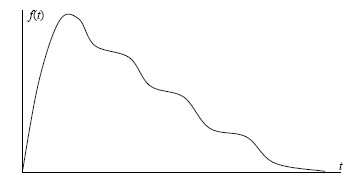
\includegraphics{TeXGraphics/Chapter1b.jpg}
	\caption{Height versus time}
	\label{Chapter1Figureb}
\end{figure}

\item In Figure \ref{Chapter1Figurec} is the graph of the function $g(t)$ that represents your distance from dorm room at time $t$.  Write an explanation of what you are doing to make the graph look like it does.%put Chapter 1 Figure b here

\begin{figure}[ht]
	\centering
		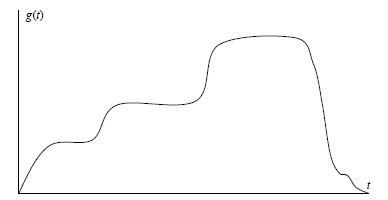
\includegraphics{TeXGraphics/Chapter1c.jpg}
	\caption{Distance from dorm room versus time}
	\label{Chapter1Figurec}
\end{figure}

\item The vertical line test provides a graphical way of determining whether a graph is a function or not.  Explain the vertical line test verbally and analytically. 

\item Consider the following forms of a quadratic function.    $$f(x) = a(x - b)(x - c)$$  $$f(x) = a(x - d)^2 + g$$  $$f(x) = ax^2 + bx + c$$    Discuss the advantages and disadvantages of each one. 

\item First, graph $$f(x)=(x-1)(x+2)(x-3)(x+4).$$  To practice using interval notation, find the intervals where $f(x)$ is positive and the intervals where $f(x)$is negative.  Explain how to do this to a friend that missed class that day.

\item Starting from a single cell, a human being is formed by 50 generations of cell division.  Explain why after $n$ divisions there are $2^n$ cells.  Guess how many cells will be present after 50 divisions.  Now compute $2^{50}$ and compare to your guess.  Briefly discuss how rapidly exponential functions increase.  \cite{SM}

\item Are there 2 functions $f$ and $g$ such that $f \circ g = g \circ f?\ \ \cite{FWG}$    

\item Are there 2 functions $f $ and $g$ such that the graphs of $f$ and $g$ are not straight lines but the graph $f \circ g$ is a straight line?  \cite{FWG}

\item If $f(x)$ is odd can anything be said of $g(x) = f(x) - 2$? If $f(x)$ is even can anything be said of $g(x) = f(x) - 2$?  \cite{FWG}

\item Explain why the graphs of $f(x) = 2^{ - x}$  and $ g(x) = \left( {{\textstyle{1 \over 2}}} \right)^x $ are the same.  \cite{SM}

\item Define a function and give examples of functions and non-functions explaining each example.

\item Give examples of each of the following functions and explain how to identify each one.  Explain how to find the domains in each class of functions.     \\   linear, constant, radical, rational, quartic, exponential

\item Describe in everyday language what the graphs of even and odd functions look like?  Explain that even and odd functions are not opposite concepts by doing the following.    \\a)  Draw a graph of a function that is neither even nor odd.    \\b)  Draw a graph of a function that is odd but not even.    \\c)  Draw a graph of a function that is even but not odd.    \\d)  Draw a graph of a function that is both even and odd.

\item Can a linear function be odd?  Can a linear function be even? 

\item a)  Can a function have more than one $x$-intercept?     \\b)  Can a function have more than one $y$-intercept?     \\c)  What do the intercepts say about the graph of a function?

\item a)  Explain why $c$ and $d$ are the $x$-intercept and $y$-intercept, respectively, of $${x \over c} + {y \over d} = 1.$$    \\b)  How are the $x$-intercept and $y$-intercept related to $c$ and $d$ in $${x \over c} + {y \over d} = 2.\ \   \cite{FWG}  $$  \\c)  Generalize.  

\item If $$f(x) = {1 \over {x + 1}},$$ what value(s) of $x$ satisfy $$f\left( {{1 \over {x + 1}}} \right) = f\left( {{{2x + 1} \over {2x + 4}}} \right).$$

\item Explain how to find the solution to $${{x - 2} \over {x + 1}} > 0$$ from the graph of $$f(x) = {{x - 2} \over {x + 1}}.$$  Describe this in a general way in order to help someone solve rational inequalities in general.

\item Choose some numbers in the domain of $$f(x) = {{\sqrt {x^2  - 1} } \over {x^2  - x - 6}}.$$  Choose some numbers that are not in the domain.  How did you find these numbers?

\item Investigate the validity of this statement:  The only graphs that are functions are those that are defined by a specific equation $y = f(x)$.

\item Explain the process of using your calculator to graph all of the circle $x^2 + y^2 = 4$.  

\item Discuss the issues of finding the domain of $f(x) = \left( {2x - 1} \right)^{ - {3 \mathord{\left/ {\vphantom {3 2}} \right. \kern-\nulldelimiterspace} 2}} .$

\item What does ``inverse'' mean?  What is an inverse function?  What are the inverse functions for each of the following?  Why is an inverse function useful?      $$\matrix{f(x) = x + 3&g(x) = 2x &h(x) = {1 \over x}\cr \cr k(x) = \sqrt x &j(x) = e^x &l(x) = \sin x\cr}$$  

\item Most of the time in mathematics, the notation we use is consistent.  However, there are times when it is not.  In particular, we use a superscript``$-1$'' to mean 2 different things.  Explain the difference in the meaning of $$x^{ - 1} \ \  {\rm{and}}\ \  \sin ^{ - 1} x.$$  What do each of these represent, how are each of these used, and how is the representation different for each?  Give other examples of the use of each notation and explain which of $$x^{ - 1} \ \  {\rm{and}}\ \  \sin ^{ - 1} x$$ each usage is like.

\item How do we prove that one function is the inverse of the other?  Why does this ``proof'' work, i.e., what is an inverse and why does this ``proof'' show that 2 functions are inverses of each other?  Give an example of a pair of functions that are inverses of each other, showing the ``proof''.  Give a second example of a pair of functions that are not inverses of each other, showing the ``proof''.

\end{enumerate}
 

\chapter{Limits and Continuity}  

 \section{General}  \begin{enumerate}  

\item  Why are polynomial functions "nice"? 

\item  Explain what it means to solve something by analytical, numerical, and graphical methods.  What is the value and limitation of each method? 

\item  Look back at the homework and writing assignments you have done so far and identify concepts that you feel you know the best.  Identify areas that you need to improve on before the exam.  If you could improve on one concept before the exam, what concept would be the most beneficial to you and why? Which are the trickiest? 

\item  We have seen that $$\mathop {\lim }\limits_{x \to a} \left[ {f\left( x \right) + g\left( x \right)} \right] = \mathop {\lim }\limits_{x \to a} f\left( x \right) + \mathop {\lim }\limits_{x \to a} g\left( x \right)$$ if the limits of $f$ and $g$ are both finite.  However, we cannot always break operations up across sums so we need to understand which can and which cannot "distribute".  Make a list of operations that you know of and decide which "distribute" across addition and which do not.  Give counterexamples for the ones that do not "distribute". 

\item  Write up to 5 distinct questions from the material in this chapter that I might ask on an exam about the following information:  $$f(x) = {x \over {\left| x \right|}}.$$

\item  Write up to 5 distinct questions from the material in this chapter that I might ask on an exam about the following information:  $$f(x) = {{\left( {x - 1} \right)^2 } \over {x^2  - 1}}.$$

\item  Write up to 5 distinct questions from the material in this chapter that I might ask on an exam about the following information.
Intermediate Value Theorem 

\end{enumerate}\section{Limits} \begin{enumerate} 

\item  A friend of yours has the following work on their paper.
$$\mathop {\lim }\limits_{x \to 0} {{\sin 3x} \over {2x}} = \mathop {\lim }\limits_{x \to 0} {{\sin 3\rlap{--} x} \over {2\rlap{--} x}} = {{\sin 3} \over 2} \approx 0.0706$$
Gently and kindly help your friend understand he has made and explain how to do the problem correctly. 

\item  A friend of yours missed class yesterday and we were talking about how to find the limits of rational functions analytically.  Explain the process to your friend. 

\item  a)  Evaluate the limit $\mathop {\lim }\limits_{x \to 0} {{e^{2x}  - 1} \over {e^x  - 1}}$ and explain each step.  \\
b) Evaluate the limit $\mathop {\lim }\limits_{x \to 0} {{e^{3x}  - 1} \over {e^x  - 1}}$ and explain each step.  \\
c)	Generalize. 

\item  Consider the function $$f(x) = {x \over {\left| x \right|}}.$$  Calculate $f(x)$ for $x$ = $-2$, $-1.5$, $-1$, $-0.5$, 0, 0.5, 1, 1.5 and 2.  Does $$\mathop {\lim }\limits_{x \to 0} f(x)$$ exist? Discuss.  

\item  Describe the limitations of finding limits by tables or graphs. 

\item  Does the existence and value of the limit of a function $f(x)$ as $x$ approaches $a$ ever depend on what happens at $x = a$?  \cite{FWG} 

\item  Evaluate $$\mathop {\lim }\limits_{x \to 0} \left[ {x^2  - {{\cos x} \over {1,000,000,000}}} \right]$$ analytically.  Explain why it would be difficult to find this limit with either graphical or numerical methods. \cite{SBS} 

\item  How are one-sided limits related to limits?  How can this relationship sometimes be used to calculate a limit or prove it does not exist?  \cite{FWG} 

\item  If $$\mathop {\lim }\limits_{x \to a} f(x) = \infty $$ does this limit exists?  Is $\infty$ a number?  Some people say that the slope of a vertical line does not exist and some say the slope is $\infty$.  Are these the same thing?  In general, talk about what $\infty$ represents and how we use this symbol. 

\item  Investigate the  validity of this statement:  If $x$ is close to zero, then so is $x^{ - 3} .$ 

\item  Investigate the  validity of this statement:  If $x$ is close to zero, then so is $x^{{1 \mathord{\left/ {\vphantom {1 3}} \right. \kern-\nulldelimiterspace} 3}} .$ 

\item  Investigate the  validity of this statement:  $\mathop {\lim }\limits_{x \to 2} x^3  = 6.$ 

\item  Investigate the  validity of this statement:  $\mathop {\lim }\limits_{x \to 0} {{\sin 2x} \over {3x}} = 1.5.$ 

\item  Is it possible for $$\mathop {\lim }\limits_{x \to a^ -  } f(x),\ \  \mathop {\lim }\limits_{x \to a^ +  } f(x),$$ and $f(a)$ to have three distinct values?  If no, explain why it is impossible.  If so, give an example of such a function $f$.  Write up how you found the function, your observations, etc. 

\item  It is probably clear that caution is important in using technology.  Equally important is redundancy.  This property is sometimes thought to be a negative (i.e., wasteful, unnecessary), but it has a positive role, nonetheless.  By redundancy we mean investigating a problem using graphical, numerical and symbolic tools.  Why is it important to use multiple methods?  Answer this from a practical perspective and a theoretical perspective (if you have learned multiple techniques, do you understand the mathematics better?)  The drawback of caution and redundancy is that they take extra time.  In computing limits, when should you stop and take extra time to make sure an answer is correct, and when is it safe to go on to the next problem?  Should you always look at a graph?  compute function values?  do symbolic work?  \cite{SM}  

\item  Note that $$\mathop {\lim }\limits_{x \to a} f(x)$$ does not depend on the value of $f(a)$, or even if $f(a)$ exists or not.  In principle, functions such as $$f(x) = \left\{ \matrix{x^2 , &  x \ne 2 \cr 13, &  x = 2}  \right.$$ are as "normal" as functions such as $$g(x) = x^2 .$$  With this in mind, explain why it is important that the limit concept is independent of how (or whether) $f(a)$ is defined.  \cite{SM} 

\item  Numerical methods help us understand limits, but if not used carefully they can lead us to incorrect answers.  Consider the function $$f(x) = \sin \textstyle{{1 \over x}}.$$\\
a)	Calculate approximations of $$x = {\textstyle{{ - 2} \over \pi }},\;{\textstyle{{ - 2} \over {9\pi }}},\;{\textstyle{{ - 2} \over {13\pi }}}\ \ {\rm{ and }}\ \ x = {\textstyle{2 \over {3\pi }}},\;{\textstyle{2 \over {7\pi }}},\;{\textstyle{2 \over {19\pi }}}$$ so you can see that these are lists of values that get closer and closer to 0.  \\
b)  Construct a table showing the values of $f(x)$ for $$x = {\textstyle{{ - 2} \over \pi }},\;{\textstyle{{ - 2} \over {9\pi }}},\;{\textstyle{{ - 2} \over {13\pi }}}\ \ {\rm{ and }}\ \ x = {\textstyle{2 \over {3\pi }}},\;{\textstyle{2 \over {7\pi }}},\;{\textstyle{2 \over {19\pi }}}.$$  Based on your results, what would you say about $$\mathop {\lim }\limits_{x \to 0} \sin \textstyle{{1 \over x}}?$$ \\
c)  Calculate approximations of $$x = {\textstyle{{ - 1} \over {2\pi }}},\;{\textstyle{{ - 1} \over {11\pi }}},\;{\textstyle{{ - 1} \over {20\pi }}} \ \ {\rm{ and }}\ \ x = {\textstyle{1 \over {5\pi }}},\;{\textstyle{1 \over {30\pi }}},\;{\textstyle{1 \over {50\pi }}}$$ so you can see that these are lists of values that get closer and closer to 0.  \\
d)  Construct a table showing the values of $f(x)$ for $$x = {\textstyle{{ - 1} \over {2\pi }}},\;{\textstyle{{ - 1} \over {11\pi }}},\;{\textstyle{{ - 1} \over {20\pi }}}\ \ {\rm{ and }}\ \ x = {\textstyle{1 \over {5\pi }}},\;{\textstyle{1 \over {30\pi }}},\;{\textstyle{1 \over {50\pi }}}.$$  Based on your results, what would you say about $$\mathop {\lim }\limits_{x \to 0} \sin \textstyle{{1 \over x}}?$$\\
e)	What do the results of both a) and b) say about $$\mathop {\lim }\limits_{x \to 0} \sin \textstyle{{1 \over x}}.  \cite{SBS} $$ 

\item  Using numerical methods to find $$\mathop {\lim }\limits_{x \to 0} {{\sin x} \over x}$$ (be careful how you enter this on the calculator).  Use a table with three values in it:  $x$, $\sin x$, and $${{\sin x} \over x}.$$  Also, draw a graph of $x$ and $\sin x$ close to 0 on the same coordinate system.  Write a paragraph explaining your work and the observations you make from the table and the graphs.  Make a reasonable argument for why the limit of $${{\sin x} \over x}$$ as $x$ approaches 0 is what it is. 

\item  Find $$\mathop {\lim }\limits_{x \to \infty } {1 \over {\sqrt {x + 1} }}\ \ {\rm{and}} \ \ \mathop {\lim }\limits_{x \to  - \infty } {1 \over {\sqrt {x + 1} }}.$$  Explain what is going on in each case. 

\item  Convert $$\mathop {\lim }\limits_{x \to \infty } f(x) = 2$$ to words.  In fact, try to rewrite this statement in as many different ways as you can in an attempt to describe what it means. 

\item  Convert $$\mathop {\lim }\limits_{x \to  - 1} f(x) = \infty $$ to words.  In fact, try to rewrite this statement in as many different ways as you can in an attempt to describe what it means. 

\item  Convert $$\mathop {\lim }\limits_{x \to \infty } f(x) =  - \infty $$ to words.  In fact, try to rewrite this statement in as many different ways as you can in an attempt to describe what it means. 

\item  Consider a polynomial function $P(x)$ of degree $n$.  Explain what to look for in $P(x)$ to determine the value of $$\mathop {\lim }\limits_{x \to \infty } P(x)$$ and $$\mathop {\lim }\limits_{x \to  - \infty } P(x).$$  Using this information (and other facts about polynomial functions), explain why a polynomial function of odd degree must have at least 1 $x$-intercept. 

\end{enumerate}\section{Continuity and the Intermediate Value Theorem} \begin{enumerate} 

\item  Explain what the Intermediate Value Theorem is, how to use it, and how it is useful. 

\item  If functions $f(x)$ and $g(x)$ are continuous for $ 0 \le x \le 1 $, could $ f(x)g(x) $ be discontinuous at a point in $ \left[0, 1\right]$?  Could $ {{f(x)} \over {g(x)}} $ be discontinuous at a point in $ \left[0, 1\right] $?  \cite{FWG} 

\item  In what ways can a function be discontinuous?  Give examples and explain what part of the definition of continuity your examples do not satisfy. 

\item  Is any real number exactly 1 less than its cube?  (Hint:  Write a mathematical statement that asks the same thing as this English statement.  Note that the question does not ask you to find the number, only to show that it exists.)  How does this question relate to the material in Chapter 2. 

\item  Is it true that a continuous function that is never zero on an interval never changes sign on that interval?  \cite{FWG} 

\item  \label{alaska} Last June I visited my sister in Fairbanks, Alaska.  One Saturday, we hiked up Chena Dome starting at 9 am.  At the top, we made camp and stayed the night.  On Sunday, we started at 9 am and started back down the hill.  Prove that at some time of day on Saturday and Sunday we were at exactly the location on the trail up Chena Dome.\\ 
	$\mbox{}\ \ \ \ \ \ $(Hint:  Draw a sketch of the function of our altitude on Saturday versus time.  On the same graph, draw a sketch of the function of our altitude on Sunday versus time.  A picture is not a proof, but it should help lead you on the right path (pun intended).)\\ 
	$\mbox{}\ \ \ \ \ \ $Note that we cannot say exactly what time of day this "crossing of paths" happened, but that is not the point.  The issue here is simply that it must have happened.  This is called an existence proof.  It is like knowing that your spouse is having an affair.  You may not know who they are having the affair with or when they met up, but you may have proof that they are having an affair, i.e., the affair exists. 

\item  Must there have been some time in your life when your height ($h$) in inches exactly matched your weight ($w$) in pounds?  For most people your age it has.  Prove that at one time they were exactly the same.   Refer to Problem \ref{alaska} for more information. 

\item  One question that we need to address in Calculus is whether an operation or procedure works when you add, multiply and divide functions.  This question asks you to find some functions to show that continuity does not "survive" addition, multiplication and division. 
\begin{enumerate} 
\item Find functions $f$ and $g$   continuous on   $(0, 1)$ such that $f + g$ is not continuous on the same interval.\\
\item Find functions $f$ and $g$   continuous on   $(0, 1)$ but for which $fg$ is not continuous on the same interval.\\
\item Find functions $f$ and $g$   continuous on   $(0, 1)$ but for which $f /g$ is not continuous on the same interval.\\ 
\item Find functions $ f$ and $g$ such that $f$ is not continuous on   (0, 1) but $f + g$ is continuous on the same interval.\\ 
\item Find functions $f$ and $g$ such that $f$ is not continuous on   $(0, 1)$ but $fg$ is continuous on the same interval.\\ 
\item Find functions $f$ and $g$ such that $f$ is not continuous on   $(0, 1)$ but $f/g$ is continuous on the same interval.\\ 
\item To turn in:  write up your examples, your observations, and the methods you used to create your examples. 
\end{enumerate}

\item  Think about the following "real-life" functions, each of which is a function of the independent variable time:  the height of a falling object, the velocity of an object, the amount of money in a bank account, the cholesterol level of a person, the heart rate of a person, the amount of a certain chemical present in a test tube and a machine's most recent measurement of the cholesterol level of a person.  Which of these are continuous functions?  For each function you identify as discontinuous, what is the real-life meaning of the discontinuities?  \cite{SM} 

\item  What conditions must be satisfied by a function if it is to be continuous at an interior point of its domain?  How does that differ from checking to see if it is continuous at an endpoint of its domain?  \cite{FWG} 

\item  What is the definition of continuity?  Explain each part of the definition.  Give an example of 4 functions:  one that is continuous and one that does not fulfill each of the parts of the definition of continuity. 

\end{enumerate}\section{Asymptotes} \begin{enumerate} 

\item  Consider a vertical asymptote of a function at $x = 2$.  Explain how to use a table of values to help you determine the limits of $f$ from the left and right of $x = 2$ and to describe the behavior of the graph of $f$. 

\item  It is rare to find simple rules in calculus.  Special (i.e., pathological) cases often exist, and we must be careful to be rigorous.  You may have heard the simple rule:  to find the vertical asymptotes of $f(x) = {{g(x)} \over {h(x)}}$  set $h(x)$ equal to 0 and solve for $x$.  Give an example where $h(a) = 0$, but there is not a vertical asymptote at $x = a$.  \cite{SM}  What can be said about the point $x = a$ with respect to the graph of $f(x)$?  Is the converse true, that is, if $x = a$ is a vertical asymptote of $y = f(x)$ is $h(a) = 0$? 

\item  Many students learn that asymptotes are lines that the graph gets closer and closer to without ever reaching.  This is true for many asymptotes, but not all.  Explain why vertical asymptotes are never crossed by the graph.  Explain why horizontal asymptotes may be crossed.  \cite{SM} 

\item  On your computer or calculator, graph $y = {1 \over {x - 2}}.$  What are the horizontal and vertical asymptotes of this curve?  Look at these asymptotes on the curve you graphed on the calculator or computer.  Most computers will draw a vertical line at the vertical asymptote and will show the graph completely flattening out at the horizontal asymptote for large values of $x$.  Is this accurate?  misleading?  Why does the vertical line appear?  Is it a part of the graph?  How can you keep the computer from drawing it?  Is the graph ever completely flat?  Why does it look that way on your computer?  \cite{SM} 

\item First, provide rough sketches of $\displaystyle y={1 \over x}$, $y=e^x$, $y=\ln x$, $y=2^{-x}$ and $\displaystyle y={1\over {x+2}}$.  Using thse graphs, explain how to find the following limts.  Make strong connections between the behavior of the graphand the value of the limits.  Where possible, explain how to evaluate the limit without having to refer to the graph.  These are limits that you should know how to evaluate relatively easily in the future, and using a grph is a useful way to ``remember'' what the limits are.
\begin{enumerate}
\item $\displaystyle\mathop {\lim }\limits_{x \to 0^ +  } \ln x$
\item $\displaystyle\mathop {\lim }\limits_{x \to 0^ +  } {1 \over x}$
\item $\displaystyle\mathop {\lim }\limits_{x \to \infty  } {e^x}$
\item $\displaystyle\mathop {\lim }\limits_{x \to -\infty  } {e^x}$
\item $\displaystyle\mathop {\lim }\limits_{x \to \infty  } {2^{-x}}$
\item $\displaystyle\mathop {\lim }\limits_{x \to -\infty  } {2^{-x}}$
\item $\displaystyle\mathop {\lim }\limits_{x \to \infty  } \ln x$
\item $\displaystyle\mathop {\lim }\limits_{x \to -2^-  } {1\over {x+2}}$
\end{enumerate}


\end{enumerate}  

 

\chapter{Derivatives}\section{General}

\begin{enumerate}

\item  An equation like $$\sin ^2 x + \cos ^2 x = 1$$ is an identity because it is true for all values of $x$.  An equation like $$2x + 5 \cos x = 1$$ is not an identity because it is only true for specific values of $x$.  If you start with an identity and differentiate both sides, the result is also an identity; if you start with an equation that is not an identity and differentiate, the result is often not an identity.  (Try this on $\sin ^2 x + \cos ^2 x = 1$ and $2x + 5 \cos x = 1$.)
 Differentiate the following to show that the results are identities.   \cite{FWG}
\begin{enumerate} 

\item  $$\sin 2x = 2\sin x\cos x$$ 

\item   $$\cos 2x = \cos ^2 x - \sin ^2 x$$ \end{enumerate}


\item  Compare and contract explicit functions and implicit functions.

\item  Compare and contrast prime notation and Leibniz notation.

\item  Compare and contrast the meaning and usage of $$f'(c)$$ and $$f'(x).$$

\item  Certain values for a differentiable function are given in the following table.  Approximate the value of $f'(0.3).$  Explain how you found this approximation and why it is only an approximation.  (Maybe sketching a graph will help).
$$\begin{array}{|c|c|c|c|c|c|c|c|c|c|}\hline  x & 0.0 & 0.1 & 0.2 & 0.3 & 0.4 & 0.5 & 0.6 & 0.7 & 0.8  \cr \hline  f(x) & 5.0 & 4.1 & 4.0 & 4.6 & 5.5 & 6.2 & 6.5 & 6.1 & 5.7  \cr \hline  \end{array}$$

\item  Explain what an independent variable and a dependent variable are.  In an explicit function, how can we identify the assumed independent variable?  Why do we need to be told which is which in an implicit function?  In a graph, how do we identify the assumed independent variable?  If we are given a set of points or a table of ordered pairs, how do we identify the assumed independent variable?

\item  I did the 36 derivatives in the review at the end of the chapter.  I copied the original problem, found the derivative, and simplified.  This took me an average 1.25 minutes per derivative.  Let's assume a first-year Calculus student 4 times as long to complete the same exercises.  Set aside a time a do as many of these derivatives as you can.  If you run into one that you cannot do right away, mark it and go on.  When you are done, check the time and your work.  If it took you more than 5 minutes times the number you got correct including simplifying, then you need to practice more before the exam. 
 To turn in, analyze the derivatives you could not do right away and the ones you got wrong.  Also, talk about the amount of time it took you to do these problems.  Look at the list of derivative techniques in the review material and decide what you know well and what you have problems with.  What do you plan to do about this?

\item  Investigate the validity of this statement:   If $f(x) \le x$, then $f'(x) \le 1.$

\item  Look back at the homework and writing assignments you have done so far and identify concepts that you feel you know the best.  Identify areas that you need to improve on before the exam.  If you could improve on one concept before the exam, what concept would be the most beneficial to you and why? Which are the trickiest?

\item  We have seen $${{d\left( {f + g} \right)} \over {dx}} = {{df} \over {dx}} + {{dg} \over {dx}}$$ but $${{d\left( {f \cdot g} \right)} \over {dx}} \ne {{df} \over {dx}} \cdot {{dg} \over {dx}}.$$  Differentiation does not ``distribute'' across multiplication.  Make a list of operations that ``distribute'' across addition and some that do not with counterexamples to justify your choices.

\item  Write up to 5 distinct questions from the material in this chapter that I might ask on an exam about the following information:  $${{dy} \over {dx}} = {{dy} \over {du}} \cdot {{dy} \over {dx}}.$$

\item  Write up to 5 distinct questions from the material in this chapter that I might ask on an exam about the following information:  differentiability.

\item  Write up to 5 distinct questions from the material in this chapter that I might ask on an exam about the following information:  $f(x) = 3e^{2x}$ at $x = 0$.

\item  Write up to 5 distinct questions from the material in this chapter that I might ask on an exam about Figure \ref{Chapter3Figurea}. %Figure goes here

\begin{figure}[ht]
	\centering
		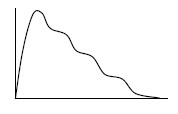
\includegraphics{TeXGraphics/Chapter3Fig.jpg}
	\caption{A graph}
	\label{Chapter3Figurea}
\end{figure}

\item  A differential helps us measure a function's sensitivity to change.  Suppose that we make a fixed small change in x, i.e., $dx$ is small and fixed.  If a small change in $x$ results in a large change in $y$, then we say the function is sensitive to change.  Since the differential gives us an approximate value for the change in $y$, then the differential also measures the sensitivity of the function. \begin{enumerate}


\item  Is $f(x) = x^3 - x$ more sensitive to small changes at $x = 0.5$, $x = 1$ or $x = 1.5$?  Explain what this means.


\item  Is $f(x) = x^2$ more sensitive to small changes than $f(x) = x^3$ is at $x = 1$?  Explain what this means.


\item  How can we quickly determine where a function is more sensitive  to change based on the graph of the derivative of the function? \end{enumerate}

\item  Explain the difference between $${{d^2 y} \over {dx^2 }}$$ and $$\left( {{{dy} \over {dx}}} \right)^2 .$$\end{enumerate}\section{Differentiability}\begin{enumerate}

\item  Compare and contrast differentiability and continuity.

\item  Describe geometrically when a function typically does not have a derivative at a point.   \cite{FWG}

\item  First, explain why $$\sqrt {x^2 }  = \left| x \right|.$$  At first glance it would appear that $$g(x) = \sqrt {x^2 } $$ is differentiable for all $x$, but we know $$f(x) = \left| x \right|$$ is not differentiable at $x = 0$.  Explain this ``paradox''.

\item  How are differentiability and continuity related?   \cite{FWG}

\item  What does it mean for a function to be differentiable?  Give three distinctly different sketches of functions that are not differentiable at particular points (make sure you indicate the point) and explain why each is not differentiable.

\item  Consider the graph of $$f(x) = \left| {\sin x} \right|.$$  Is this graph continuous?  If not, why not and where?  Is this graph differentiable?  If not, why not and where? \end{enumerate}\section{Tangent Lines}\begin{enumerate}

\item  For what values of $a$ and $b$ is $2x + y = b$ tangent to $y = ax^2$ at $x = 2$?  

\item  The line $L$ is tangent to the graph of the differentiable function $y = f(x)$ at the point (5, 2).  $L$ intersects the $y$-axis at (0, 4).  Find $f'(5).$  Provide an illustration along with the writing.

\item  What does it mean for a line to be tangent to a curve $C$ at a point $P$?   \cite{FWG}

\item  What is the relationship between secant lines and tangent lines?

\item  A friend says that if a straight line touches a curve at exactly one point, then it is tangent to the curve at that point. Your friend also says that if a straight line touches a curve at more than one point, then it cannot be tangent to the curve at any of those points.  What do you think?

 \end{enumerate}\section{Methods of Differentiation}\begin{enumerate}

\item  Compare and contrast the evaluation of the derivatives of the following functions.
\begin{enumerate}

\item  $y = 3^3$ 

\item   $y = x^3$ 

\item  $y = x^x$ 

\item   $y = 3^x$\end{enumerate}

\item  A friend of yours says that since the derivative of $f(x) = x^2 - 4x$ at $x = 2$ is 0 that means that $f(x) = x^2 - 4x$ is a constant function.  Help your friend understand this better.

\item  A student was absent from class today and asked you to help him understand when and how to use logarithmic differentiation.  Give him several examples that do not need logarithmic differentiation and several that do.  Explain the process.

\item  A student was absent from class yesterday and asked you to help him understand the chain rule.  In particular, he needs help understanding how to find the derivatives of $\sin 5 x$ and $\sin x^5$.  Explain this to him.

\item  As a mathematical quiz show contestant, you are asked to find the value $$F'\left( 7 \right)$$ for the composition $$F = f \circ g.$$  The functions $f$ and $g$ are unknown, but you are permitted to ask exactly 3 questions to help you find the answer.  What 3 questions should you ask?  \cite{EP}

\item  Compare and contrast the evaluation of the derivatives of $$e^{x\sin x} ,$$ $$e^x \sin x$$ and $$xe^{\sin x} .$$

\item  Compare and contrast the product and the quotient rules.

\item  Create a concept map of the derivatives of the trigonometric functions that emphasizes the symmetry and patterns of the derivatives.  Describe these patterns in words. 

\item  Create some new derivative rules based on the rules we have learned so far.  First, if $$y = {1 \over u},$$ what is $${{dy} \over {dx}}?$$  This would be called the Reciprocal Rule.  Also, if $y = uvw$, what is $${{dy} \over {dx}}?$$  This is the Triple Product Rule.  What would the Quadruple Rule be?  

\item  Derive a general formula for the derivative of $$y = f(x)^{g(x)} .$$  Make comparisons to the rules for the derivatives of $$u = a^{g(x)} $$ and $$v = f(x)^b .$$

\item  Each time we use implicit differentiation we are able to rewrite the resulting equation in the form $$f(x,y) = y' \cdot g(x,y)$$ for some expressions $f$ and $g$.  Explain why this can always be done; that is, why doesn't the chain rule ever produce a term like $$(y')^2 $$ or $${1 \over {y'}}?  \ \cite{SM}$$   

\item  Explain how to derive the derivative formula for $$y = \sin ^{ - 1} x.$$

\item  Explain what needs to be true about a function for you to need the chain rule?  Give examples of functions that need the chain rule and functions that do not need the chain rule.  Be as inclusive as possible.

\item  Many students prefer the product rule to the quotient rule.  Explain how each can be used to find the derivative of $$f(x) = {{\left( {2x - 3} \right)^4 } \over {\left( {x - 1} \right)^3 }}.$$  Which do you prefer and why?

\item  Once you know the derivatives of $\sin x$ and $\cos x$, how can you find the derivatives of 
$\tan x$, $\cot x$, $\sec x$, and $\csc x$?   Choose an example to annotate.   \cite{FWG}

\item  Suppose $$F(x) = f\left( {g\left( {h(x)} \right)} \right).$$  Write out the chain rule for $$F'\left( x \right).$$  What numerical values would be needed to find $$F'\left( 7 \right)? \ \cite{EP}$$    Write out the chain rule for $$G(x) = f\left( {g\left( {h\left( {m\left( x \right)} \right)} \right)} \right).$$ What numerical values would be needed to find $$G'\left( 2 \right)?$$

\item  Using that $$\left( {\sin x} \right)^\prime   = \cos x$$ and $$\left( {\cos x} \right)^\prime   =  - \sin x,$$ derive the formulas for $\tan x$, $\cot x$, $\sec x$, and $\csc x$.  When we take the derivative of $\cos x$, the sign of the result is opposite of the original.  Also, note that $\tan x$, $\cot x$, and $\csc x$ have $\cos x$ in their definitions.  Which of the derivatives result in a change of sign?  Why don't all of the derivatives of the trigonometric functions with $\cos x$ in their definition result in a change of sign?  Develop a mnemonic to help you remember these rules. 

\item  We can find the derivative of certain exponential functions without the chain rule.  Compare and contrast calculating the derivative of $$f(x) = e^{2x} $$ using the chain rule and using the product rule on $$f(x) = e^{2x}  = \left( {e^x } \right)\left( {e^x } \right).$$  Do the same with $$f(x) = e^{3x} .$$

\item  We usually talk about trigonometric functions in pairs.  Cosine is paired with sine, tangent is paired with secant and cotangent is paired with cosecant.  Describe a trigonometric relationship and a calculus relationship to justify each pairing.

\item  You and a friend compared answers to your homework.  Your friend found the derivative of $$p = {{\tan t} \over {1 + \tan t}}$$ and got $${{dp} \over {dt}} = {1 \over {1 + \sin 2t}}$$ which doesn't look anything like your answer.  If you are both right, explain how each of you got the answer and why they are the same.  If one of you is wrong, explain the error and how to avoid it in the future.

\item  You found the derivative of $$M(x) = {{2x - 3} \over {x^3 }}$$ and got $$M'(x) = {{9 - 4x} \over {x^4 }}.$$  You decided to check your answer with a friend's answer and she got $$M'(x) =  - 4x^{ - 3}  + 9x^{ - 4} .$$  Should either of you be worried?  Which answer is ``better''?  

\item  You have been cautioned against multiplying out the terms of a derivative.  Explain why having a factored form of $$f'\left( x \right)$$ is helpful.  How close does the product rule bring you to a nicely factored form of $$f'\left( x \right)? \  \cite{SM}
$$  
\item  A friend of yours has the following work on their paper.
 $$\displaylines{  f(x) = x^{ - {3 \mathord{\left/ {\vphantom {3 2}} \right. \kern-\nulldelimiterspace} 2}}  \cr   f'(x) =  - {{3x^{ - {1 \mathord{\left/ {\vphantom {1 2}} \right. \kern-\nulldelimiterspace} 2}} } \over 2} \cr} $$
Gently and correctly help your friend understand the mistake he made and give him advice about how to avoid this mistake in the future.

\item  A friend of yours has the following work on their paper.
 $$\displaylines{  f(x) = {{\sin x} \over x} \cr   f'(x) = 1 \cr} $$
Why do you think your friend made this mistake?  Gently and correctly help your friend understand the mistake he made and give him advice about how to avoid this mistake in the future.

\item  Compare and contrast the evaluation of the derivatives of $$\sin ^2 x$$ and $$\sin x^2 .$$

\item  Compare and contrast the evaluation of the derivatives of $${{x^3  - 1} \over {x^2 }}$$ and $${{x^2 } \over {x^3  - 1}}.$$

\item  Consider the relationship $x^2 + y^2 = 100$ where $y < 0$.  Use implicit differentiation to find $${{dy} \over {dx}}.$$  Now, solve for $y$ and find $${{dy} \over {dx}}$$ in the usual way.  Show that the results are the same.  Would the results be the same if we did not restrict y to be negative?  Why do we need implicit differentiation?

\item  Using the definition of 
$$\left| a \right| = \left\{ \begin{array}{ll} a, & \,a \ge 0 \cr    - a, & \,a < 0 \cr \end{array} \right.,$$ write a piecewise definition of $$y = \ln \left| x \right|.$$  Now, find $$y'.$$  Observations? 

\end{enumerate}\section{Graphs and the Derivative}\begin{enumerate}

\item  Consider the function $f(x)$, its vertical translation $g(x) = f(x) + a$, and its horizontal translation $h(x) = f(x + a)$.  How do the derivatives of $g$ and $h$ compare to the derivative of $f$?  Explain how the graphs of the function and its translations confirm your analytic results.

\item  Consider the graph of $y = f'(x)$ in Figure \ref{Chapter3a}.  Of the 5 points marked on the graph, choose and label the point where $f(x)$ is the largest. Of the 5 points marked on the graph, choose and label the point where $f(x)$ is the smallest.  Can you approximate those values of $f(x)$?  Explain why you made the choices you did.   %put figure 1 here

\begin{figure}[ht]
	\centering
		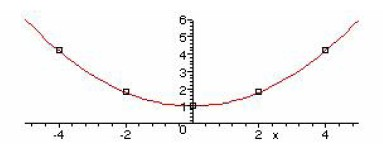
\includegraphics{TeXGraphics/Chapter3a.jpg}
	\caption{Approximating derivatives}
	\label{Chapter3a}
\end{figure}




\item  Consider the graph of $y = f(x)$ in Figure \ref{derivativegraph}.  Create axes and scales for this graph.  Mark and label on the graph the point at which $f'(x)$ has the greatest positive value,  the point at which $f'(x)$ has the smallest absolute value and the point at which $f'(x)$ has the greatest negative value.  Approximate those values?  Explain your work.                       %put DerivativeFunction.jpg here
\begin{figure}[ht]
	\centering
		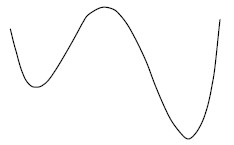
\includegraphics{TeXGraphics/DerivativeFunction.jpg}
	\caption{Extreme derivatives}
	\label{derivativegraph}
\end{figure}


\item  Does the curve $y = x^3$ ever have a negative slope?  If so, where?  If not, justify your answer.  What does this say about the shape of the curve?

\item  Find the angle between the circle $x^2 + y^2 = 1$ and the circle $x^2 + (y - 1)^2 = 1$ at each of the two points of intersection.

\item  How does the graph of $-f(x)$ compare to the graph of $f(x)$?  How does the value of $ - f'(a)$ compare to $f'(a)?$   How does the graph of $3f(x)$ compare to the graph of $f(x)$?  How does the value of $3f'(a)$ compare to $f'(a)?$  Be sure to talk about the connection between the derivative and slope.

\item  Investigate the validity of this statement:  If the derivative of a function is positive in a given interval, then the function is increasing.

\item  Use graphical analysis to argue that the derivative of $\cos x$ is $-\sin x$.   \cite{SM}

\item  Investigate the validity of this statement:  If $f(p)$ and $f(q)$ are both absolute minimum values of $f$ on its domain, then $f(p) = f(q)$.   \cite{EP}

\item  Investigate the validity of this statement:  Relative minima can occur at many different locations, but the absolute minimum can only occur at one location.

\item  Investigate the validity of this statement:  Every local extreme of the function $f$ occurs at a point where $$f'(x) = 0.$$  Does the answer change if we replace the word ``local'' with ``global''?

 \end{enumerate}\section{Applications of the Derivative}\begin{enumerate}

\item  A friend of yours missed the first day we talked about related rates problems and wants to know what we did so he can complete the homework.  Rewrite and improve Example 1 from this section of the test to help explain the process to him.  

\item  A linear approximation to $f$ at $x_0$ is a line $L(x) = ax + b$ where $$L\left( {x_0 } \right) = f\left( {x_0 } \right)$$ and $$L'\left( {x_0 } \right) = f'\left( {x_0 } \right).$$  What if we wanted to approximate the curve with a parabola instead of a line.  Consider the quadratic function $$Q\left( x \right) = ax^2  + bx + c$$ and the curve $$f\left( x \right) = \left( {1 - x} \right)^{ - 1} $$ and the point $$x_0  = 0.$$  Find the coefficients $a$, $b$ and $c$ so that $$Q\left( {x_0 } \right) = f\left( {x_0 } \right),$$ $$Q'\left( {x_0 } \right) = f'\left( {x_0 } \right),$$ and $$Q''\left( {x_0 } \right) = f''\left( {x_0 } \right).$$  Graph $f$ and $Q$.  Zoom in on the point $$x_0  = 0.$$  Comment on what you see. If the results of the graph are not as expected, then something is amiss.  How does this quadratic approximation compare to a linear approximation?

\item  Choose a specific related rates problem and use dimensional analysis to show that the units work out correctly.

\item  Compare and contract implicit differentiation and differentiation in related rates problems.

\item  Compare and contrast rectilinear motion problems and related rates problems.

\item  Compare and contrast the concepts of position, distance, and displacement within the scope of rectilinear motion.

\item  Consider a general linear function $L(x) = ax + b$.  Show that if $L$ is a linearization of $f$ at $x_0$, then $$L\left( {x_0 } \right) = f\left( {x_0 } \right)$$ and $$L'\left( {x_0 } \right) = f'\left( {x_0 } \right).$$  Explain why this must be true.

\item  Describe a situation that can be solved using related rates methods.  Explain what is happening to each variable and each rate at a specific time.  How would looking at the same situation at a different time impact the variables and rates?

\item  Discuss error propagation, including relative error, and percentage error.   \cite{SBS}

\item  How do derivatives arise in the study of motion?  What can you learn about a body's motion along a line by examining the derivatives of the body's position function?   \cite{FWG}

\item  How do related rate problems arise?   \cite{FWG}

\item  If you are doing a related rates problem and you find that one of the dependent variables is constant, what happens?  Using an example of your own choice show that it doesn't matter whether you know the variable is constant before you start or later in the problem.

\item  Linearization can give us ``good'' approximations or ``bad'' approximations.  Explain why it can be said that $y = x$ is a good approximation to $y = \sin x$ near $x = 0$ but $y = 1$ is not a good approximation to $y = \cos x$ near $x = 0$.   \cite{SM}

\item  Tangent line approximations are useful only if $\Delta x$ is small.  Consider the approximation of $$y = \sqrt x $$ only using the linearization of $$y = \sqrt x $$ at the point $x = 81$.  Make a table of values of approximations and actual values of $$y = \sqrt x $$ for various values of $x$ around $x = 81$.  What other calculations might you make?  What values would be good to have in your table (I can think of several)?  Discuss your observations.

\item  The equations for free fall at the surfaces of Vulcan and Kronos are $s = 1.86t^2$ meters and $s = 11.44t^2$ meters, respectively, where $t$ is time in seconds.  How long does it take a rock falling from rest to reach a velocity of 27.8 m/sec on each planet?  Which planet has ``stronger'' gravity?  How can you determine that from the equations and/or graphs alone?

\item  Using the definition of the derivative, explain why the units of velocity are distance/time and why the units of acceleration are ${\rm{distance}}/({\rm{time}})^2$.

\item  What is a differential?  What is it used for?  What are the notational alternatives to using a differential and why, in some cases, is a differential an advantage over the alternative?

\item  What is the difference between speed and velocity?  We use both of these words in our every day language, but one of them we usually use incorrectly.  Which one is it?  What does acceleration mean in terms of speed?  Why do we call the accelerator the accelerator in our car?  Is it always used as an accelerator in the mathematical sense of the word?  How else does acceleration happen when we are driving a car?

\item  What is the function that gives the height of an object shot straight up from the ground at an initial velocity of 30 feet/sec?  Graph this function.  Find the  velocity and acceleration functions and graph them, too.  Identify the important features of the graphs and describe what is happening at those points.  Explain why the acceleration function looks the way it does.  (What would it say about the Earth if the acceleration function looked different than it does?  Have you ever seen the movie Hypercube?)

\item  When we differentiate with respect to $t$ for related rates, we can use any form of the equation as long as we keep note the domain.  For example, differentiate $$d = \sqrt {x^2  + y^2 } $$ with respect to $t$.  Now, conveniently change the equation and differentiate again.  Show that the 2 results are the same thing.  How could this be useful when using related rates?

\item  For rectilinear motion we use a function and its first and second derivatives.  What information do we obtain from the original function and what types of questions can we answer with it?  The first derivative?  The second derivative?

\item  Why is it important to identify the independent variable before finding a derivative?  What is the independent variable in a related rates problem?  How does this impact how we solve a related rates problem?  
\end{enumerate}\section{Higher Order Derivatives}\begin{enumerate}

\item  Find constants $A$, $B$, and $C$ so that $$y = Ax^3  + Bx + C$$ satisfies the equation $$y''' + 2y'' - 3y' + y = x.$$  

\item  Find the derivative of $y = \sin x$ of many different orders.  From this data, determine an algorithm for finding any derivative of $y = \sin x$.  Explain your algorithm so others can use it.  Find $${{d^{123} y} \over {dx^{123} }}.$$  Find $${{d^{708} y} \over {dx^{708} }}.$$

\item  What is a second derivative?  A third derivative?  How many derivatives do the functions you know have?   \cite{FWG}

\item  Consider a polynomial of degree $n$.  Describe as fully as possible, all the derivatives of this polynomial of any order.
\end{enumerate}
 

\chapter{Applications of the Derivative}
\section{General}\begin{enumerate}

\item  Describe briefly as many applications of derivatives as you can.  Organize these applications in a concept map. 

\item  Determine if each of the following is always true or not always true.  If it is always true, give an argument to support your claim.  If it is not always true, give a counterexample.  
\begin{enumerate}
	\item 	If $f$ is differentiable at $a$, then $$\mathop {\lim }\limits_{x \to a} f(x)$$ exists.
	\item	If $f(c)$ is a local maximum of $f$, then $f'(c) = 0.$
	\item	If $(c, f(c))$ is an inflection point, then $f(c)$ is not a local maximum of $f$.  \cite{MR}
\end{enumerate}

\item  I have a pet polynomial function and I never learned how to share very well so ``You can't have it!''  My mother always says that nobody likes a smart aleck (not her exact words) but you have a chance to be one if you can tell me as much about what my pet function looks like without even knowing what the function is.

\item  If $f'\left( x \right) \le 2$ for all $x$, what is the largest possible increase in the values of $f$ on $[0, 6]$?

\item  Look back at the homework and writing assignments you have done so far and identify concepts that you feel you know the best.  Identify areas that you need to improve on before the exam.  If you could improve on one concept before the exam, what concept would be the most beneficial to you and why? Which are the trickiest?

\item  Write up to 5 distinct questions from the material in this chapter that I might ask on an exam about the following information: Mean Value Theorem.

\item  Write up to 5 distinct questions from the material in this chapter that I might ask on an  about the following information: $f(x) = 3x^3 - 6x$.

\item  Write up to 5 distinct questions from the material in this chapter that I might ask on an exam about the following information:  maxima, minima.

\end{enumerate}\section{Extremes and Optimization}\begin{enumerate}

\item  A friend of yours has missed class (again!) and needs to know how to find absolute extrema.  Gently explain the procedure to her by going through an example.  

\item  Compare the extrema of the 2 functions $f(x)$ and $g(x)$ such that $f(x) - g(x) = 5$ for all $x$. 

\item  Explain the conditions under which a graph is guaranteed to have an absolute maximum and absolute minimum.  Show, using examples, that those conditions are necessary (i.e., if you eliminate one condition, find a graph that does not have the absolute extrema.)

\item  Explain the difference between relative extrema and absolute extrema.  If we consider functions on $(-\infty, \infty)$, are we guaranteed to find relative extrema? If we consider functions on $(-\infty, \infty)$, are we guaranteed to find absolute extrema? If we consider functions on a closed interval, are we guaranteed to find relative extrema? If we consider functions on a closed interval, are we guaranteed to find relative extrema?  Compare and contrast each of these situations.

\item  Find the maximum value of $f(x) = x^3  - 3x$ on the set of real numbers $x$ satisfying $x^4  + 36 \le 13x^2 .$

\item  If $f'(a) < 0 < f'(b)$ and $a < c < b$, is $c$ guaranteed to be a maximum as in the first derivative test?

\item  If $f''(c) > 0$ is c guaranteed to be a minimum as in the second derivative test?

\item  Is it true that a discontinuous function cannot have both an absolute maximum and an absolute minimum value on a closed interval?  \cite{FWG}

\item  It can be said that $$g(x) = \sqrt {f(x)} $$ is minimized by exactly the same $x$-values(s) as $f(x)$ (for $f(x) \ge 0$).  Explain why this is true and for which of the following functions it is also true.
\begin{enumerate} 
	\item $g(x) = \ln \left( {f(x)} \right)$ for $f(x) > 0$	
	\item $g(x) = \left( {f(x)} \right)^2 $	
	\item $g(x) = e^{f(x)} $
	\item $g(x) = \sin \left( {f(x)} \right)$
	\item $g(x) = \left( {f(x)} \right)^3 $
\end{enumerate}

\item  It is important to understand mathematical language and one way to test your knowledge is to ask for specific information in a problems.  In a problem about relative extrema, I could ask for critical numbers, critical values, maximum value, minimum value, or the location of the maximum or minimum.  In each case explain how you know whether to give an $x$-value, a $y$-value, or an ordered pair.

\item  Suppose some friends complain to you that they can't work any of the optimization problems in the book.   When you ask to see their work, they say that they couldn't even get started.  It has been emphasized in class that sketching a picture and defining variables is a good start.  Part of the benefit of this is to help you get started writing something (anything) down.  Do you think this advice helps?  What do you think is the most difficult aspect of these problems?  Give you friends the best advice you can.  \cite{SM}

\item  We have a theorem that says that a continuous function on a closed interval has an absolute maximum and minimum.  But remember that to apply a theorem, the hypotheses have to be checked first.  What happens if we eliminate one of those hypotheses?  Consider a discontinuous function on a closed interval.
\begin{enumerate}
	\item Find such a function with a minimum but no maximum.
	\item Find such a function with a maximum but no minimum.
	\item Find such a function with neither a maximum nor minimum.
	\item Find such a function with both a maximum and minimum.  \cite{SBS}
	\item Discuss your observations.
\end{enumerate}

\item  We have a theorem that says that a continuous function on a closed interval has an absolute maximum and minimum.  But remember that to apply a theorem, the hypotheses have to be checked first.  What happens if we eliminate one of those hypotheses?  Consider a continuous function on an open interval.
\begin{enumerate}
	\item  Find such a function with a minimum but no maximum.
	\item Find such a function with a maximum but no minimum.
	\item Find such a function with neither a maximum nor minimum.
	\item Find such a function with both a maximum and minimum.  \cite{SBS}
	\item Discuss your observations. 
\end{enumerate}

\item  We know how to find the extreme values of a continuous function $f(x)$ by investigating its values at critical points and endpoints..  But what if there are no critical points of endpoints?  What happens then?  Do such functions really exist?  \cite{FWG}

\item  What is the difference between a critical point and a critical number?  Compare and contrast the processes for finding critical numbers in the case of relative extrema on 
$(-\infty, \infty)$ versus absolute extrema on $[a, b]$.  How does this distinction help us eliminate work in application problems?

\item  What is the first-derivative test?  How do you use it?  Why does it work?  What does it tell you?  What do you need to be careful about?\end{enumerate}\section{Rates of Change}\begin{enumerate}

\item  Consider this problem: Find 2 nonnegative numbers so that the sum of the first and twice the other is 12 and the product is a maximum.  In this problem, what is the function you are trying to optimize?  What is the constraint(s)?  Explain these 2 equations, how you use them, their relationship to each other, how you know which is which, etc.

\item  Consider this problem: What is the largest possible area for a right triangle whose hypotenuse is 5 cm long?  In this problem, what is the function you are trying to optimize?  What is the constraint(s)?  Explain these 2 equations, how you use them, their relationship to each other, how you know which is which, etc.

\item  Sam the bartender prepares Norm and Cliff each a Scotch and Water.  The percentage concentration of pure scotch in their drinks is 6.25\%.  Each has an infinitely large glass.

\begin{enumerate}
	\item Before Norm has a chance to start drinking, Vera starts adds water to his drink at a constant rate.  Draw a graph that represents the percentage concentration of pure scotch as a function of the number of ounces of water added by Vera to Norm's drink.  Is this function concave up or down?
	\item Before Cliff has a chance to start drinking Carla calls Cliff a wimp, grabs his drink and adds pure scotch to it at a constant rage.  Draw a graph that represents the percentage concentration of pure scotch as a function of the number of ounces of water added by Vera to Cliff's drink.  Is this function concave up or down? 
\end{enumerate}

\item  Suppose that $f(t)$ represents your elevation after $t$ hours on a mountain hike.  If you stop to rest, explain why $$f'(t) = 0$$ at that point.  Discuss the circumstances under which you would be at a local maximum, local minimum or neither.  \cite{SM}

\item  Two crash test dummies are testing a '72 Pinto station wagon that has been refitted with airbags.  Listen to them, plot their velocity function, and then answer these questions.  What is the domain of the velocity function?  On what interval is Mack and Biff's velocity increasing?	 On what interval is their velocity decreasing?  Is this a continuous function?
\\ {\bf{Mack}}:  Turn the car on, Biff, and let's get going.  We've got an appointment with that brick wall 400 meters ahead.
\\ {\bf{Biff}}:  So, I'm supposed to speed up to 30 m/sec?
\\ {\bf{Mack}}:  Yeah.  When we reach that speed we should be 250 meters down the track.  And then we maintain that speed until we are 50 meters in front of the wall.
\\ {\bf{Biff}}:  And then we slow down so that we hit the wall going 25 m/sec, right?
\\ {\bf{Mack}}:  Riiiiiiggggghhhhhhhhtttttttt!!!!!!!   

\item  What can you say about the rate of change of a constant function?  A linear function?  An exponential function?  A power function?  \cite{SMo}

\item  What is the formula for the volume of a cube?  Its surface area?  What is the formula for the volume of a sphere?  Its surface area?  Find the rate of change of the volume of a cube with respect to the length of one of its edges.  How does this compare to the surface area of the cube?  Find the rate of change of the volume of a sphere?  How does this compare to the surface area of the cube?

\end{enumerate}\section{Mean Value Theorem}\begin{enumerate}

\item  Compare and contrast Rolle's Theorem (RT) and the Mean Value Theorem (MVT).  

\item  Compare and contrast the Intermediate Value Theorem (IVT) and the Mean Value Theorem (MVT).  

\item  Your pesky friend has missed class one more time.  This time he missed the discussion on the Mean Value Theorem (MVT).  After giving him a tactful and gentle lecture on attending class and abusing your friendship, carefully and clearly explain the hypotheses and conclusion of the MVT to him.  Give him some examples of graphs to show what the hypotheses mean.  Using a graph, explain the conclusion of the MVT to him.

\item  Explain how the Mean Value Theorem can be used to prove that, if $f'\left( x \right) = 0$ for all $x$, then $f$ is a constant function.

 \end{enumerate}\section{Graphs and the Derivative}\begin{enumerate}

\item  Apply the second derivative test to $f(x) = x^4$ at the critical number $x = 0$.  Discuss.

\item  If $f'(c) = 0$, is $(c, f(c))$ guaranteed to be an extreme?   Explain and then describe how to determine if $(c, f(c))$ is an extreme?  

\item  Back in the dark ages when I first learned the $x$-coordinate of the vertex of a parabola 
$y = ax^2 + bx + c$ was $$x =  - {b \over {2a}},$$ I didn't know why it worked.  Here you will prove this result is in 2 different ways.

\begin{enumerate}
	\item Assume that a parabola is symmetric.  So the vertex will fall exactly halfway between the $x$-intercepts.  Find the average of the x-intercepts of $y = ax^2 + bx + c$.  
	\item The vertex of a parabola is at the point on the curve where the tangent is horizontal.  Use calculus to find the $x$-coordinate of the vertex.
\end{enumerate}


\item  Can the graph of a function have more inflection points than critical points?  \cite{EP}

\item  Consider the function $f(x) = 5x^2	+ 13x - 6$.  Graph this function on the interval $(-3, 3)$.  Select 5 different values of $x$ from the interval $(-3, 3)$ and place those values in a table in ascending order.  Draw the tangent line to the graph for each value of $x$ you chose.  Find the slope of these tangent lines and enter the slopes in the table.  As you move from left to right on the graph, are the slopes of the tangent lines increasing or decreasing?  What does this say about the derivative of $f'(x)?$    

\item  Consider the function $f(x) = \ln x$ . Graph this function on the interval $(-1, 5)$. Select 5 different values of $x$ from the interval $(-1, 5)$ and place those values in a table in ascending order.  Draw the tangent line to the graph for each value of $x$ you chose.  Find the slope of these tangent lines and enter the slopes in the table.  As you move from left to right on the graph, are the slopes of the tangent lines increasing or decreasing?  What does this say about the derivative of $f'(x)?$

\item  Describe the relationship of the graph of the derivative to the graph of the function. \cite{SBS}

\item  Find constants $A$, $B$, $C$ and $D$ that guarantee that the graph of $$f(x) = 3x^4  + Ax^3  + Bx^2  + Cx + D$$ will have horizontal tangents at $(2, -3)$ and $(0, 7)$.  There is a third horizontal tangent; find it.  Then, for all 3 points, determine whether each corresponds to a relative maximum, a relative minimum, or neither.  \cite{SBS}

\item  Find the critical points of $$f(x) = 2x^3  + 3x^2  - 12x + 11.$$  Apply the first derivative test to $$f(x) = 2x^3  + 3x^2  - 12x + 11$$ to classify these critical points.  Apply the second derivative test to $$f(x) = 2x^3  + 3x^2  - 12x + 11$$ to classify these critical points.  Compare and contrast the application of these 2 tests.  In your writing, consider the application of these tests to more complicated functions.  Are there any functions for which either test fails?

\item  Find the domain of the graph $$f(x) = x^{{2 \mathord{\left/ {\vphantom {2 3}} \right. \kern-\nulldelimiterspace} 3}} \left( {5 - 2x} \right).$$  What does this tell us about the appearance of the graph?  Now graph this function on your calculator.  Is the result consistent with what the graph should look like?  If it is not, find a way to make the calculator do the right thing.  (Remember you are smarter than the calculator.)

\item  For each of the following, try to sketch the function.  If you can sketch it, explain its features and their relationship to the values of the derivatives.  If you cannot sketch it, explain what the contradiction is.\begin{enumerate}
\item A continuous function on $[a, b]$ with a critical point $c$ between $a$ and $b$ but with no extreme value on $(a, b)$.		
\item A differentiable function on $[a, b]$ with a critical point $c$ between $a$ and $b$ but with no extreme value on $(a, b)$.
\item A continuous function on $[a, b]$ with 2 critical points between $a$ and $b$ but with no extreme value on $(a, b)$. 	
\item A continuous function on $[a, b]$ with a local minimum and a local maximum but only one critical point in $(a, b)$.  \cite{EP} \end{enumerate}

\item  For each of the following, try to sketch the function.  If you can sketch it, explain its features and their relationship to the values of the derivatives.  If you cannot sketch it, explain what the contradiction is.
\begin{enumerate}
\item A continuous function on $[a, b]$ with a local minimum and a local maximum and exactly 3 critical points in $(a, b)$.		
\item A continuous function on $[a, b]$ with 3 local maxima but only a single local minimum in $(a, b)$.
\item A function that has 2 distinct critical points that are not separated by an inflection point?  \cite{EP}  \end{enumerate}

\item  For each of the following, try to sketch the function.  If you can sketch it, explain its features and their relationship to the values of the derivatives.  If you cannot sketch it, explain what the contradiction is.
\begin{enumerate}
\item A function which is increasing on $(-\infty, \infty)$ and has a maximum at $x = 2$.		
\item A function that is always negative and always increasing.
\item A function with 2 $x$-intercepts and no minima. 	
\item A function with no $x$-intercepts and no $y$-intercepts. \end{enumerate}

\item  For each of the following, try to sketch the function.  If you can sketch it, explain its features and their relationship to the values of the derivatives.  If you cannot sketch it, explain what the contradiction is.
\begin{enumerate}\item A function with exactly 2 maxima and no minima.	
\item A continuous function with exactly 2 maxima and no minima.
\item A function with no extrema.	
\item A significantly different function with no extrema. \end{enumerate}

\item  For each of the following, try to sketch the function.  If you can sketch it, explain its features and their relationship to the values of the derivatives.  If you cannot sketch it, explain what the contradiction is.
\begin{enumerate}\item A polynomial of odd degree that has neither a local minimum value nor a local maximum value. 	
\item A polynomial function of even degree that has neither an absolute minimum value nor an absolute maximum value.  \cite{EP} \end{enumerate}

\item  For this writing assignment you need to first complete the following experience.  You will work in groups of 3.  
\\ {\bf{Round 1}}:  {\bf{Step 1}}:  Student A sits back-to-back with student B while student C is in a position to watch what is going on.  Student A is given a graph and has to describe that graph to Student B.  Student B will try to reproduce the graph by listening to Student A.  Students B and C cannot talk except that Student B can ask Student A to slow down or to continue.  Student C should monitor the process and keep everyone on task.  
\\ {\bf{Step 2}}: After Student A has described the graph and B has drawn it, compare the graphs.
\\{\bf{Step 3}}:  In your group discuss how the describing/drawing went and make plans for improving the process.
\\{\bf{Rounds 2 and 3}}:  Repeat Round 1 except that each student must assume a new role.  At the end of the 3 rounds each student must have been a describer once, a drawer once, and an observer once.
\\{\bf{To turn in}}: After reviewing the process, how would you recommend as the best way to describe the graph.  Provide details and possibly examples.

\item  If $f'(x)$ does not exist at $x = a$, does that guarantee that $a$ is a critical number for $f$?

\item  If $f''(c) = 0,$ is $c$ guaranteed to be an inflection point?  If $f''(c) \ne 0,$ is it guaranteed that  $c$ is not an inflection point?

\item  If a statement is false, give a counterexample.  If a statement is true, explain why. \begin{enumerate}
\item If $f$ is concave up, then $-f$ is concave down.
\item If $f$ is concave up and $g$ is concave up, then $fg$ is concave up.
\item If $f$ is concave up and $g$ is concave down, then $fg$ is neither concave up nor down. \end{enumerate}

\item  If I ask you to match graphs of derivatives to graphs of functions, what do you look for?

\item  On what intervals is $f$ increasing and decreasing if $${{df} \over {dx}} = 6\left( {x - 1} \right)\left( {x - 2} \right)^2 \left( {x - 3} \right)^3 \left( {x - 4} \right)^4 .$$  What are the extrema of $f$?  \cite{FWG}

\item  Prove or disprove:  If the graphs of $f$ and $g$ are both concave up on an interval, then the graph of their sum $f + g$ is also concave up on that interval.  \cite{SBS}

\item  Sketch a curve for which $f(x) < 0$, $f'(x)< 0$, and $f'(x)$ is decreasing on $(-\infty, \infty)$.

\item  In the following graph one of the curves is $f(x)$ and the other curve is its derivative.  Which is which?  Explain your answer. 
%put Chapter4Fig.jpg here

\item  Let $$f(x) = \root 5 \of {x^3  - Lx + 1} $$ where $L$ is the number of letters in your last name.  Let $g(x)$ be another function such that the tangent line to $g(x)$ at $x = 2$ is $y = 7x - 4S$, where $S$ is the number of sisters you have.  For which of the following functions can we determine the tangent line from the above information?  If it is possible to determine it, do so.  If there is not enough information to determine it, explain why not. \cite{FWG}
\begin{enumerate}
	\item $A(x) = f(x) + g(x)$ at $x = 2$ 
	\item $B(x) = f(x) g(x)$ at $x = 2$
	\item $C(x) = f(x)/g(x)$ at $x = 2$ 
	\item $D(x) = f(g(x))$ at $x = 2$
	\item $E(x) = g(f(x))$ at $x = 2$
\end{enumerate}

\item  Let $$f(x) = x^4  + x^3  - 8x^2  - 12x.$$  Find the first and second derviatives of $f(x)$.  Discuss whether each of the following statements is true or false. \begin{enumerate}
\item $f$ is increasing at $x = 1$.
\item $f$ has a relative minimum at $x = -2$.
\item $f$ is concave down at $x = 1$.
\item $f$ has a root at $x = 1$.  \cite{SMo}\end{enumerate} 

\item  Suppose that you have a differentiable function $f(x)$ with 2 critical numbers.  You computer has shown you a graph that looks like Figure \ref{Chapter4Figureb}.  Is it possible that there are any important points not shown in the window you used to display this graph?  Would your answer change if the function had 3 critical numbers?  \cite{SM}

%put Chapter4Figb.jpg here

\begin{figure}[ht]
	\centering
		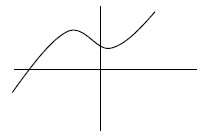
\includegraphics{TeXGraphics/Chapter4Figb.jpg}
	\caption{A function}
	\label{Chapter4Figureb}
\end{figure}

\item  The goal of investing in the stock market is to buy low and sell high.  But, how can you tell whether a price has peaked or not?  Once a stock price goes down, you can see that it was at a peak but then it is to late to do anything about it!  Concavity can help.  Suppose a stock price is increasing and the price curve is concave up.  Why would you suspect that it will continue to rise?  Is this a good time to buy?  Now, suppose the price is increasing but the curve is concave down.  Should you be preparing to sell?  Buy?  Finally, suppose the price is decreasing.  If the curve is concave up, should you buy or sell?  What if the curve is concave down?  \cite{SM}

\item  The upcoming exam will require you to understand graphing and will have some pretty involved multi-step problems.  First, complete this problem:  ``Consider the function $$f(x) = \root 3 \of x \left( {27 - x} \right).$$  Graph this function by first listing all key features.  Pay attention to how easy or difficult each part of this problem is.  Did you remember all the key features?  If you could improve one part of these problems, what area would be the most beneficial to you and why?  What parts are the easiest for you?  Which are the trickiest?

\item  What is the relationship between $x$-intercepts and the intervals where a function is positive and negative?  What is the relationship between extrema and the intervals where a function is increasing and decreasing?  What is the relationship between inflection points and the intervals where a function is concave up and down?

\item  What is the second-derivative test?  How do you use it?  Why does it work?  What does it tell you?  What do you need to be careful about?

\item  Compare and contrast the graphs of polynomial and rational functions.

\item  Graph $$f(x) = \left| x \right|$$ on the interval [-1, 2].  What is the sign of $$f'\left( x \right)$$ on (-1, 0)?  What is the sign of $$f'\left( x \right)$$ on (0, 2)?  Can we apply the First Derivative Test to $f(x)$ on [-1, 2]?

\item  Fill in the blank and then explain your choices:  Every $\mathop {\underline {\quad \quad \quad \quad \quad } }\limits_{{\rm{global}}\ \  {\rm{or}}\ \   {\rm{local}}} $
 maximum of the function $f$ is also a $\mathop {\underline {\quad \quad \quad \quad \quad } }\limits_{{\rm{global}}\ \  {\rm{or}}\ \  {\rm{local}}} $
 maximum of $f$.

\item  Consider a polynomial function $P(x)$ of degree $n$.  What is the maximum number of $x$-intercepts $P$ could have?  The maximum number of critical points?  The maximum number of inflection points?  Is it possible for a polynomial to attain the maximum number of inflection points but only have 1 critical point (possible of a high multiplicity)? 

\end{enumerate}\section{Asymptotes}\begin{enumerate}

\item  Compare and contrast horizontal and vertical asymptotes.  Include both analytical and visual examples to illustrate the points you make.  Discuss the examples numerically.

\item  Explain why polynomials never have  vertical or horizontal asymptotes.  \cite{SM}

\item  Find constants a and b that guarantee that the graph of the function defined by $$f(x) = {{ax + 5} \over {3 - bx}}$$ will have a vertical asymptote at $x = 5$ and a horizontal asymptote at 
$y = -3$. \cite{SBS}  In general, discuss how the values of $a$, $b$, $c$ and $d$ determine the horizontal and vertical asymptotes of $$f(x) = {{ax + d} \over {bx + c}}.$$

\item  Find the horizontal and vertical asymptotes of a variety of rational functions.  Make conjectures that would help you find these asymptotes without all the fuss.

\item  If $x = 2$ is a vertical asymptote of the graph of the function $y = f(x)$, describe what happens to the $x$- and $y$-coordinates of a point moving along the graph, as $x$ approaches 2.

\item  There are other types of asymptotes than just vertical and horizontal.  Before looking at slant and polynomial asymptotes, let's first look at a new way to look at vertical asymptotes.  Find the (right) horizontal asymptote $y = a$ of $$f(x) = {{2x} \over {3x + 1}}.$$  Now calculate the limit $$\mathop {\lim }\limits_{x \to \infty } \left[ {f(x) - a} \right].$$  Try this for several other rational functions.  Look at the graphs of $f(x)$ and $y = a$ and describe their relationship for large values of $x$.
	\\\mbox{}$\ \ \ \ \ $Find a linear function $l(x) = ax + b$ such that $$\mathop {\lim }\limits_{x \to \infty } \left[ {f(x) - l(x)} \right] = 0$$ for the function $$f(x) = {{x^3  + 2x^2  - 1} \over {x^2  - 1}}.$$  Graph $f(x)$ and $l(x)$ and describe their relationship for large values of $x$.  The line $l(x)$ is called a slant asymptote.  Make a general description of rational functions that have slant asymptotes.
	\\\mbox{}$\ \ \ \ \ $For each of these functions, find a polynomial $P(x)$ such that $$\mathop {\lim }\limits_{x \to \infty } \left[ {f(x) - P(x)} \right] = 0.$$




\begin{enumerate}
\item $f(x) = {{x^4 } \over {x + 1}}$
\item $f(x) = {{x^5  - 1} \over {x + 1}}$
\item $f(x) = {{x^6  - 2} \over {x + 1}}\ \ \cite{SM}$  
\end{enumerate}
Graph each $f(x)$ and $P(x)$ and describe their relationship for large values of $x$.  These polynomials are called polynomial asymptotes.  Make a general description of rational functions that have polynomial asymptotes.

\item  While studying for an exam, a friend says that a graph is not allowed to touch an asymptote.  What do you think?

\item  Investigate the validity of this statement: When finding horizontal asymptotes you only have to calculate $$\mathop {\lim }\limits_{x \to \infty } f(x)$$ because $$\mathop {\lim }\limits_{x \to  - \infty } f(x)$$ is always the same thing. 

\item  Investigate the validity of this statement:  Every rational function has vertical asymptotes.

\item  Investigate the validity of this statement:  A graph cannot have both a vertical asymptote and a slant asymptote.

\end{enumerate}\section{L'Hospital's Rule and Indeterminate Forms}

\begin{enumerate}

\item  Explain in your own words why $0^\infty  $ and $0^{ - \infty } $ are not indeterminate forms.  \cite{EP}  Be sure to explain what an indeterminate form is and why these two forms do not fit in that category.  As always, examples where these 2 forms occur would be useful.

\item  How do you use L'Hospital's Rule?  When can you apply it?  What does it help us do?  What happens if you apply it at times when you shouldn't?  Using a picture, give an overview of why L'Hospital's Rule works.

\item  What is an indeterminate form?  Give examples of indeterminate forms and of forms that are not indeterminate.  What distinguishes these 2 forms?  Give examples to illustrate what makes an indeterminate form indeterminate.

\item  A friend of yours has this work on their paper.  
		$$\begin{array}{rcl} \displaystyle{\mathop {\lim }\limits_{x \to 0} {{1 - \cos x} \over {\sec x}} }&\mathop  {=} \limits^H 
&  \displaystyle{\mathop {\lim }\limits_{x \to 0} {{\sin x} \over {\sec x\tan x}} }\cr \mbox{}&&\cr   
		&=& \displaystyle{\mathop {\lim }\limits_{x \to 0} {{\sin x} \over {\sec x\tan x}}} \cr \mbox{}&&\cr   
		&=& \displaystyle{\mathop {\lim }\limits_{x \to 0} {{\cos x} \over {\sec x}} }\cr     \mbox{}&&\cr   
		&= &\displaystyle{{1 \over 1}} \cr  \mbox{}&&\cr   
		&=&1\end{array} $$
Show them with the graph of $$f(x) = {{1 - \cos x} \over {\sec x}}$$ that they probably got the wrong limit.  Help them understand the problems in their calculations.

\item Consider the following calculation of  $\displaystyle
\mathop {\lim }\limits_{x \to \infty } \left( {1 + {\textstyle{2 \over x}}} \right)^x 
$.  Explain what has been done in each step of the calculation and why.

$$
\begin{array}{rcl}
  L 
  	&= 
  		&\mathop {\lim }\limits_{x \to \infty } \left( {1 + {2 \over x}} \right)^x  \cr 
  		\ln L
  	& =
  		& \mathop {\lim }\limits_{x \to \infty } \ln \left( {1 + {2 \over x}} \right)^x  \cr 
   	&=
   		& \mathop {\lim }\limits_{x \to \infty } x\ln \left( {1 + {2 \over x}} \right) \cr 
   	&=
   		& \mathop {\lim }\limits_{x \to \infty } {{\ln \left( {1 + {2 \over x}} \right)} \over {e{1 \over x}}} \cr 
  	&\mathop  = \limits^H &\mathop {\lim }\limits_{x \to \infty } {{{1 \over {1 + {2 \over x}}} \cdot \left( { - {2 \over {x^2 }}} \right)} \over { - {1 \over {x^2 }}}} \cr 
  	& =
  		& \mathop {\lim }\limits_{x \to \infty } {2 \over {1 + {2 \over x}}} \cr 
  	& =
  		& 2 \cr 
  \ln L 
  	&= 
  		&2 \cr 
  L
  	& =
  		& e^2  \cr 
  		\end{array}
$$


\item  Compute $$\mathop {\lim }\limits_{x \to 0^ +  } x^x $$ graphically, numerically, and analytically.  Compare, contrast and reconcile these three methods.  \cite{SBS}


\item  Let 
$$f(x) = \left\{ \begin{array}{lcr}  x + 2, 
     &\ \ \mbox{}& x \ne 0 \cr   
     0, & &x = 0 \cr \end{array}  \right.$$ 
and 
$$g(x) = \left\{ \begin{array}{lcr}  x + 1, 
     &\ \ \mbox{}& x \ne 0 \cr   
     0, & & x = 0 \cr \end{array} \right. .$$  
Show that $$\mathop {\lim }\limits_{x \to 0} {{f'(x)} \over {g'(x)}} = 1$$ and $$\mathop {\lim }\limits_{x \to 0} {{f(x)} \over {g(x)}} = 2.$$  
Why does this not contradict L'Hospital's Rule?  \cite{FWG}


\item  L'Hospital's Rule is not some magic tonic that will work for any limit.  Discuss the issues with the following limits in regard to L'Hospital's Rule.
\begin{enumerate}\item $\mathop {\lim }\limits_{x \to 1} {{x - 1} \over {\left| {x - 1} \right|}}$ \item $\mathop {\lim }\limits_{x \to \infty } {x \over {\sqrt {x^2  - 1} }}$ \item $\mathop {\lim }\limits_{x \to 0} {{1 - \cos x} \over {x^2 }}$ \item $\mathop {\lim }\limits_{x \to 1} {{x^{10}  + 1} \over {x - 1}}$\end{enumerate}

\item  L'Hospital's Rule states that, in certain situations, the ratios of function values approaches the same limit as the ratios of corresponding derivatives (rates of change).  Graphically, this may be hard to understand.  The get a handle on this, consider $${{f(x)} \over {g(x)}}$$ where both 
$f(x) = ax + b$ and $g(x) = cx + d$ are both linear functions.  Explain why the value of $$\mathop {\lim }\limits_{x \to \infty } {{f(x)} \over {g(x)}}$$ should be the same as $$\mathop {\lim }\limits_{x \to \infty } {{f'(x)} \over {g'(x)}}.\ \cite{SM}$$ 

\item  List as many indeterminate forms as possible.  Why are these forms called indeterminate?  For which of these forms can we use L'Hospital's Rule directly?  How would you transform the other indeterminate forms into ones that we can use L'Hospital's Rule?

\item  When we try to evaluate a limit and find a form such as $${\infty  \over \infty }$$ this is called indeterminate because there exist limits of this form for which the result is any real number.  Explain how to find examples of differentiable functions $f$ and $g$ such that $$\mathop {\lim }\limits_{x \to \infty } f(x) = \infty $$ and $$\mathop {\lim }\limits_{x \to \infty } g(x) = \infty $$ such that the limits have the values listed below.
\begin{enumerate}\item	$\mathop {\lim }\limits_{x \to \infty } {{f(x)} \over {g(x)}} = 3$\item		$\mathop {\lim }\limits_{x \to \infty } {{f(x)} \over {g(x)}} = 0$\item		$\mathop {\lim }\limits_{x \to \infty } {{f(x)} \over {g(x)}} = \infty $  \cite{FWG}\end{enumerate}

\item  You and a friend decide to compare homework and you find the following results.
\begin{center}{Your friend's paper}\end{center}
	$$\begin{array}{rcl}  \displaystyle{\mathop {\lim }\limits_{x \to 3} {{x - 3} \over {x^2  - 3}}}& = &\displaystyle{\mathop {\lim }\limits_{x \to 3} {1 \over {2x}}} \cr  \mbox{}&&\cr  &= &{1 \over 6} \cr \end{array}$$

\begin{center}Your paper\end{center}
$$\begin{array}{rcl}  \displaystyle{\mathop {\lim }\limits_{x \to 3} {{x - 3} \over {x^2  - 3}}} &=& \displaystyle{{0 \over 6}} \cr   \mbox{}&&\cr  &=& 0 \cr\end{array} $$
Who is right?  \cite{FWG}

\item  Your favorite friend (the one that misses class all the time) has asked you to explain how to find $$\mathop {\lim }\limits_{x \to 0} x^{\sin x} .$$  You decide it would be a good review for you to kindly show him the steps and explain them along the way.

\item  Consider the following limit:  $$\mathop {\lim }\limits_{x \to \infty } x\ln \left( {{{x - 1} \over {x + 1}}} \right) = \infty  \cdot 0 = 0.$$  Using a table, investigate whether this limit was calculated correctly.  Observations?

\item  Consider the following limit:  $$\mathop {\lim }\limits_{x \to \infty } \sqrt {x^2  + 3x}  - x = \infty  - \infty  = 0.$$  Using a table, investigate whether this limit was calculated correctly.  Observations?

\item  Consider the following limit:  $$\mathop {\lim }\limits_{x \to 0^ +  } x^{\tan x}  = 0^0  = 0.$$  Using a table, investigate whether this limit was calculated correctly.  Observations?

\item  The graphs of differentiable functions $f$ and $g$ are shown in Figure \ref{Chapter4Figurec}.  Which of the following is true about $$\mathop {\lim }\limits_{x \to 0} {{f(x)} \over {g(x)}}?$$ \begin{enumerate}\item The limit is less than 0.  \item   The limit is 0.  
\item The limit is 1. \item The limit is greater than 1.  \item The limit does not exist. \end{enumerate}
Explain your solution.  Create another figure similar to Figure \ref{Chapter4Figurec} that would use the same reasoning but would arrive at another answer on the list.  Explain the solution.

%put Chapter4Figc.jpg here
\begin{figure}[ht]
	\centering
		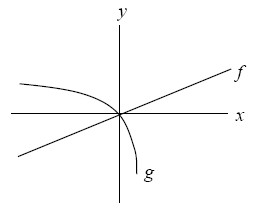
\includegraphics{TeXGraphics/Chapter4Figc.jpg}
	\caption{Two functions}
	\label{Chapter4Figurec}
\end{figure}

\item Provide an annotated calculation of $$
\mathop {\lim }\limits_{x \to 1} x^{{1 \mathord{\left/
 {\vphantom {1 {(1 - x)}}} \right.
 \kern-\nulldelimiterspace} {(1 - x)}}} .
$$


\end{enumerate}


 

\chapter{Integration}\section{General}\begin{enumerate} 


\item Show that $${d \over {dx}}\left( {{x \over {x + 1}}} \right) = {d \over {dx}}\left( {{{ - 1} \over {x + 1}}} \right).$$  Is $${x \over {x + 1}} = {{ - 1} \over {x + 1}}$$ an identity (i.e., is it true for all $x$)?  What does this say about antiderivatives?  Other comments and observations?  \cite{FWG}

\item \begin{enumerate} 

\item   	Can a function have more than one derivative? Explain.


\item   Can a function have more than one antiderivative?  Explain.


\item   What does this say about derivatives and antiderivatives?\end{enumerate}

\item   We do not (yet) have a formula for the antiderivative of some simple functions, including $\ln x$, $\sec x$, and $\csc x$.  Given $f(x)$, explain when we have a simple formula for $$\int {f(x)\,} dx.$$  For example, why is there a formula for $$\int {\sec x\tan x\,dx} $$ but not for $$\int {\sec x\,dx}.\ \ \cite{SM} ?$$  

\item   What is the ``+ C'' thing?  What purpose does it serve?  

\item   Verify that $$\int {xe^{x^2 } dx}  = {\textstyle{1 \over 2}}e^{x^2 }  + c$$ and $$\int {xe^x dx}  = xe^x  - e^x  + c$$ by computing derivatives of the proposed antiderivatives.  Which derivative rules did you use?  Each of the integrands is of the form $$f(x)g(x).$$  Identify $f$ and $g$ in each case.  Why does this make it unlikely that we will find a general antiderivative rule for $$\int {f(x)g(x)\,} dx\ ? \  \cite{SM}$$

\item   Create a concept map including the concepts of functions, derivatives, second derivatives, and integrals.  What would be a natural extension of these concepts?

\item   We have second derivatives.  What about second integrals?  What would this mean?  Create some examples.  Speculate what a second integral would measure.

\item   What are the domain of the functions $$f(x) = {1 \over x},\  \ g(x) = \ln \left| x\right| \ \  {\rm{and}}\  \ h(x) = \ln x?$$  Using these domains, explain why $$\int {{{dx} \over x} = \ln \left| x \right| + C} $$ instead of $$\int {{{dx} \over x} = \ln x + C} .$$

\item   Find the equation for the curve in the $xy$-plane that passes through the point $(1, -1)$ if its slope at $x$ is always $3x^2 + 2$.  \cite{FWG}

\item   A friend of yours has the following work on his paper.
	$$\displaylines{  \int {x^2 \left( {x^3  - 1} \right)dx}  = {{x^3 } \over 3}\left( {{{x^4 } \over 4} - x} \right) + C \cr    = {{x^7 } \over {12}} - {{x^4 } \over 3} + C \cr} $$
Gently and clearly, explain to your friend the mistake he has made and give him advice for avoiding this mistake in the future.\end{enumerate}

\section{Fundamental Theorem of  Calculus}\begin{enumerate}

\item A friend of yours has the following work on her paper.  Keeping the same antiderivative that your friend has found, explain to her what her error is and why it is an error.  Why did she make this error, and how can she avoid it in the future?
$$
\int\limits_0^4 {\left( {x - 2} \right)^2 dx}  = \left. {{{\left( {x - 2} \right)^3 } \over 3}} \right|_0^4  = {{\left( {4 - 2} \right)^3 } \over 3} = {8 \over 3}.
$$


\item   Evaluate the following definite integrals.  Your answers will be functions.
	\begin{enumerate} \item  	$f(x) = \int\limits_2^x {\left( {3t^2  + 2t} \right)\;dt} $	\item	$g(u) = \int\limits_0^u {\sin x\;dx} $	\item	$h(t) = \int\limits_{ - 1}^t {e^y \;dy} $\end{enumerate}
Since each of the integrals above is a function of a variable, we can find the derivatives.  Find the first derivative of the functions you created above.
	\begin{enumerate} \item $f'(x)$  	\item $g'(u)$	\item $h'(t)$\end{enumerate}
Observations?  State a general rule (use mathematical notation to clarify your general rule, i.e., ``If $f(x) = \int\limits_a^x {F(t)\;dt} $ where $a$ is a constant, then $f'(x) = \underline {\quad \quad \quad \quad } .'')$

\item   Using the function $$f(x) = \int\limits_0^{x^2 } {\cos t\;dt} $$ illustrate the use of the chain rule in combination with the second Fundamental Theorem of Calculus.  To do this, first evaluate the integral in the usual way and then find $f'(x)$ in the usual way.  After that, show how to find $f'(x)$ directly from $$f(x) = \int\limits_0^{x^2 } {\cos t\;dt} $$ using the second Fundamental Theorem of Calculus.  Finally, highlight in each case where the chain rule was applied making connections between the two calculations.

\item   Explain the difference between a function being integrable and being able to apply the Fundamental Theorem of Calculus (FTOC) to evaluate the definite integral of a function.  Is there a function $f(x)$ such that $y = f(x)$ is integrable but we cannot use the FTOC to directly evaluate $$\int_a^b {f(x)\,dx} ?$$  If so, how would we find the value of $$\int_a^b {f(x)\,dx} ?$$ without the FTOC?  

\item Is it difficult to determine if a function in this class is integrable or not?  Is it difficult to determine if we can apply the FTOC of calculus to a function?  Discuss.

\item   What does integrable mean?  Is it necessary for a function to be continuous to be integrable?  Is it necessary for a function to be differentiable to be integrable?  Discuss the continuity and differentiability of the functions ${\left| x \right|}$ and $f(x)$ in the integrals below.  Are ${\left| x \right|}$ and $f(x)$ in the following integrands integrable?  Explain how to evaluate these integrals.
\begin{enumerate}
\item $\int_{ - 2}^4 {\left| x \right|\,dx} $ 
\item $\int_{ - 2}^2 {f(x)dx} $ 
	where 
		$f(x) = \left\{ \begin{array}{ll}  3x, & x < 0 \cr   x^2  + 2, & x \ge 0 \cr \end{array} \right.$
\end{enumerate}

\item   Which of the following functions satisfy the Fundamental Theorem of Calculus on the intervals indicated?  If the function and interval do not satisfy the FTC, which can you calculate the integral in some other way?  
\begin{enumerate}\item $\int_0^1 {\left| {2x - 1} \right|\,dx} $ \item $\int_{ - 1}^1 {{{dx} \over {x^2 }}} $ \item $\int_{ - 1}^1 {{{dx} \over {1 + x^2 }}} $ \item $\int_{ - 1}^1 {e^{ - x^2 } dx} $ \end{enumerate}

\end{enumerate}\section{Substitution}\begin{enumerate}

\item   Explain the relationship of the chain rule for differentiation and substitution for integration.







\item   You were going over the homework with a friend and saw the following work on his paper.
		$$\begin{array}{rclcrcl}
\int_{ - 1}^2 {\left( {3x - 2} \right)^5 dx} & =& {1 \over 3}\int_{ - 1}^2 {u^5 dx} &\ \ \ \ \ \ \mbox{}& u &=& 3x - 2 \cr  
  & =& \left. {{1 \over 3}\left( {u^6 } \right)} \right|_{ - 1}^2 &&  du &=& 3dx \cr  
  &  =& {1 \over 3}\left( {2^6  - \left( { - 1} \right)^6 } \right) &&  {1 \over 3}du &=& dx \cr    
  &= &21&& \cr\end{array}$$
Your friend was very happy because the answer came out to be a whole number and that is always a good sign.  You did not like having to break the news to your friend about the mistakes you found, so you gently explained the errors and how to fix them.

\item   Sometimes a substitution is not always obvious.  Investigate the following possible substitutions for $$\int {{{x\,dx} \over {1 + x^4 }}} .$$	
\begin{enumerate} \item $u = 1 + x^4$\item $u = x^2$\item $u = x^3$\item $u = x^4$\end{enumerate}
Which substitution would be the best?  Provide some advice to another student for how to recognize the appropriate substitution.  Create other similar integrals that would benefit from the advice you gave.

\item   When we use substitution to evaluation a definite integral we have the choice of changing the limits of integration from values of $x$ to values of $u$ before the final evaluation or we can back substitute and do the final evaluation with values of $x$.  Discuss the possible advantages and disadvantages of each method.  \cite{EP}

\item   Given $$\int_0^2 {f(x)\,dx}  = 3$$ and $$\int_2^4 {f(x)\,dx}  = 5,$$ explain and illustrate the calculation of $$\int_0^2 {f(2x)\,dx} .$$  

\end{enumerate}\section{Areas, Averages and the Mean Value Theorem}\begin{enumerate}



\item Provide an annotate illustration and example of a Riemann sum.

\item Discuss the role of $n$, the number of subdivisions, in a Riemann sum.

\item Give the Definition of the Definite Integral and explain how this limit and sum might give the area under a curve.




\item   Sketch the graph of $$y = x^{{3 \mathord{\left/ {\vphantom {3 2}} \right. \kern-\nulldelimiterspace} 2}} $$ on the interval [0, 4].  Use the grid option on your calculator, and make your sketch on a grid.  When asked to make an estimate, give an upper and lower bound and discuss the method of estimation.

\begin{enumerate}


\item   Estimate the area of the region bounded by $y = x^{{3 \mathord{\left/ {\vphantom {3 2}} \right. \kern-\nulldelimiterspace} 2}} ,$ the $x$-axis, and $x = 4$.


\item   Estimate the average value $y = x^{{3 \mathord{\left/ {\vphantom {3 2}} \right. \kern-\nulldelimiterspace} 2}} $ on the interval [0, 4].

\item Calculate the area and average.  Discuss your observations.  \cite{SMo}

\end{enumerate}

\item   Explain and illustrate the average value of $x^3 - 3x^2$ on $[-2, 1]$.

\item   Find $c$ such that $$\int_a^b {f(x)\,dx}  = f(c)\left( {a - b} \right)$$ for $$f(x) = x^2  + 4x + 1$$ on [0, 2].  Explain and illustrate what it is you just calculated.  Make connections to average values and the Mean Value Theorem for Integrals.

\item   How are the Mean Value Theorem for derivatives and the Mean Value Theorem for integrals the same?  How are they different?

\item   Explain the average of a continuous function $f(x) > 0$ over the interval $[a, b]$.  Make a connection between the area bounded by $y = f(x)$, $x = a$, $x = b$ and the $x$-axis and the average value of $f(x)$ on $[a, b]$.  Using a graph, illustrate how the value $c$ from the Mean Value Theorem for Integrals (MVTI) is related to the average value.
\end{enumerate}\section{Numerical Integration}\begin{enumerate}

\item   If we are approximating areas under curves with some numerical method (rectangles, trapezoids, etc.), we have to first choose the number of subintervals to break the interval into.  What is the value of using many subintervals?  What is the problem with using many subintervals (consider that you are doing this by hand)?

\item   The Fundamental Theorem of Calculus is useful if we have a ``nice''  function $f(x)$ to integrate over an specific interval.  However, if we want to calculate the area of an object that has no nicely defined function, we can use numerical integration.  Explain how to use the trapezoid rule to find the area of Figure \ref{Chapter5Fig} by finding the area using 4 trapezoids.  Illustrate your response showing the trapezoids.  Discuss how much error you think there is in your calculation.  How could you eliminate some of that error?

\begin{figure}[ht]
\centering		
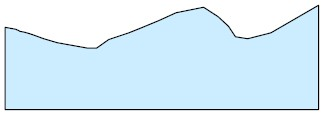
\includegraphics{TeXGraphics/Chapter5Fig.jpg}	
\caption{Area under a curve}	
\label{Chapter5Fig}\end{figure}



\item   Which of the trapezoid rule or Simpson's Rule should give a better approximation to the area under a "nice" function?  Justify your response with an illustration.

\item   Compare and contrast the processes of approximating error with rectangles, trapezoids and Simpson's Rule.

\item   Why is numerical integration important?  Are there any definite integrals you would be faced with now that you would have to use numerical integration to find a value?  What is it about these definite integrals that makes them different than the ones we studied at the beginning of the semester?

\end{enumerate}
 

\chapter{Applications of Integration}
\section{Area between curves}\begin{enumerate}

\item  How is finding the area under a curve the same as finding the area between 2 curves?  How is it different?

\item You and a friend are comparing homework, and you were assigned a problem to find the area bounded by the two curves $y = x + 1$ and  $
y = x^3  + x^2  - x + 1$.  You found the area of two separate regions and added them together.  Your friend says that whenever there are two regions, you can just find the area of one of them and double it.  Which one of you is correct?

\item  The area between $f(x)$ and $g(x)$ and between $x = a$ and $x = b$ is given by $$\int_a^b {\,\left[ {f(x) - g\left( x \right)} \right]\,dx} $$ (with appropriate assumptions about $f$, $g$, $a$ and $b$).  What happens if either $f$ or $g$ has an $x$-intercept?  Do we need to do anything different?  Why or why not?

\item  The formula $$\int\limits_I {\left[ {f\left( x \right) - g\left( x \right)} \right]\,dx} $$ is supposed to give the area of region that lies between the curves $y = f(x)$ and $y = g(x)$ and ``above'' the interval $I$ on the $x$-axis.  For this formula to work, do $f$ and $g$ both have to be positive functions?  Explain why this works just as well when $g(x) < 0 < f(x)$ and when $g(x) < f(x) < 0$.

\item  Consider the function $f(x) = \cos x$ on $[0, \pi]$ shown in Figure \ref{Chapter6Fig}.  When we find the area bounded by $y = \cos x$, $x = 0$ and $x = \pi$ (shown below) we have to break the calculation into 2 integrals.  Why?  Do we have to do the same thing when we find the average of  $y = \cos x$ on $[0, \pi]$?

 \begin{figure}[ht]
	\centering
		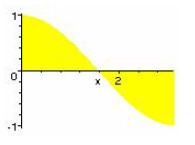
\includegraphics{TeXGraphics/Chapter6Fig.jpg}
	\caption{Area between a curve and the $x$-axis}
	\label{Chapter6Fig}
\end{figure}
 
 
 \end{enumerate}\section{Volumes of revolution}\begin{enumerate}

\item  Consider the region bounded by $y=\sqrt{x}$ and $y=x^2$.  Further, consider two solids:  one where this region is revolved about the $x$-axis and the other where this region is revolved about the $y$-axis.  Finally, consider finding these 2 volumes each in 2 different ways:  in terms of $x$ or in terms of $y$.  Set up all 4 integrals and compare and contrast the methods.

\item Compare and contrast the methods of cylindrical shells, washers and disks.

\item  Verify, using integral methods of finding volumes, that the volume of a right circular cylinder is $$V = \pi r^2 h.$$  

\item  Suppose that the region bounded by $$y = x^3  - 3x - 1$$ and $y = -4$,$-2 \le  x \le  2$, is revolved about $x = 3$.  Explain what would be necessary to compute the volume using the method of washers, and what would be necessary to use the method of cylindrical shells.  Which method would you prefer and why?

\begin{figure}[ht]
	\centering
		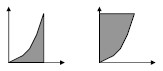
\includegraphics{TeXGraphics/VolRevCom.jpg}
	\caption{Regions to Revolve About Both Axes}
	\label{fig:volrev}
\end{figure}


\item In Figure \ref{fig:volrev} there are two regions.  Each is bounded on one edge by $y=2x^2$ and the point in the upper-right hand corner of each is $(1, 2)$.  Suppose that each region is revolved about each axis to result in 4 different solids.
\begin{enumerate}
\item First, rank the 4 solids in order by size by inspection.
\item Now, check your answer by calculating the volume of all 4 solids.
\item Discuss your ability to predict relative volume.  Observations?
\end{enumerate}


\end{enumerate}\section{Polar curves and areas}\begin{enumerate}

\item  It is easy to algebraically describe and graph spirals using polar coordinates using a polar equation such as $r=\theta$.  Why is this difficult in rectangular coordinates?  Why it is easy in polar coordinates?  How does this reflect on the value of using polar coordinates.

\item  Graph $$r = a\sec \theta $$  for several values of $a$.  What did you find?  Prove that $r=a\sec\theta$ is always a vertical line.  (Hint:  draw a triangle on the polar graph.)   What polar equation will give horizontal lines?  \cite{FWG}

\item  Discuss a procedure for finding the intersection of 2 curves in polar form.  \cite{SBS}  Compare and contrast this method to finding the intersection of 2 curves in rectangular form?

\item  Compare and contrast points given by rectangular coordinates, $(x,y)$, with points given by polar coordinates, $(r, \theta)$.

\item  Compare and contrast the process for finding the area under a curve given in rectangular form and the area enclosed by a polar curve.


\end{enumerate}\section{Arc Length and Surface Area}\begin{enumerate}

\item  What is the formula for finding the length of a segment of a curve $y = f(x)$ on $[a, b]$?  Explain, in general terms, the derivation of this formula.  What hypotheses about $y=f(x)$ must be checked first and what would you do if those hypotheses were not satisfied?


\item  What is the formula for finding the surface area which results from rotating $y = f(x)$ on 
$[a, b]$ about the $y$-axis?  Explain, in general terms, the derivation of either formula.  What hypotheses about $y=f(x)$ must be checked first and what would you do if those hypotheses were not satisfied?

\item Compare and contrast the following 4 formulas:  
\begin{enumerate}
\item  the surface area of $y = f(x)$ revolved about the $x$-axis integrated in term of $x$,
\item  the surface area of $y = f(x)$ revolved about the $x$-axis integrated in term of $y$,
\item  the surface area of $y = f(x)$ revolved about the $y$-axis integrated in term of $x$ and
\item  the surface area of $y = f(x)$ revolved about the $y$-axis integrated in term of $y$,
\end{enumerate} 

\item  Some texts recommend the formula $$L = \int_\alpha ^\beta  {\sqrt {dx^2  + dy^2 } } $$ for the arc length of a smooth curve.  Show that if the function is defined as $y = f(x)$ this formula gives us $$\int_a^c {\sqrt {1 + \left[ {f'\left( x \right)} \right]^2 } dx} $$ and if the function is defined as $x = g(y)$ this formula give us $$\int_b^d {\sqrt {1 + \left[ {g'\left( y \right)} \right]^2 } dy} .$$  Why would $$L = \int_\alpha ^\beta  {\sqrt {dx^2  + dy^2 } } $$ be easier to remember?  How was $$L = \int_\alpha ^\beta  {\sqrt {dx^2  + dy^2 } } $$ derived?

\item  Notice that the integral for arc length of the function $y = f(x)$ on $[a, b]$ is relatively complicated.  I can't just pick any function $y = f(x)$ for you to use on the exam, because I need to have a integral that is ``nice''.  Investigate using 3 elementary functions for $f(x)$ in the arc length formula.  Are the integrals easy to evaluate?

\item  Notice that the integral for the surface area of the function $y = f(x)$ on $[a, b]$ rotated about the $x$-axis is relatively complicated.  I can't just pick any function $y = f(x)$ for you to use on the exam, because I need to have a integral that is ``nice''.  Investigate using 3 elementary functions for $f(x)$ in the surface area formula.  Are the integrals easy to evaluate?

\item  Compare and contrast the formulas for finding the length of an arc of $y = f(x)$ and the formula for finding the surface area of that arc when it is revolved around the $y$-axis.

\end{enumerate}

\section{Work and Centroids}\begin{enumerate}

\item  We have used integrals $\left( {\int\limits_I {f(x)\,dx} } \right)$ to measure length and area and volume, among other measurements.  Why is it possible to use this one mathematical operation to make such diverse measurements with completely different dimensions?

\item  Explain Hooke's Law for springs.  What do we mean by the displacement of a spring?  

\item  Compare and contrast work and force.  If I am holding the calculus book still 4 feet off the floor, is it work or force?  If an elevator moves 3 people from one floor to another, is it work or force?  If a dam is holding water, is it work or force?  

\item  Complete a dimensional analysis on the formula for a centroid of a homogenous lamina.

\item  In general, what does the centroid of a homogeneous lamina represent?  Where is the centroid of a homogeneous circular lamina?  Square lamina?  A lamina that in the shape of an equilateral triangle? 

\item  What type of unit is a joule (i.e., what does it measure)?  What does a joule ``feel'' like?  Find an everyday object and an everyday distance to illustrate what 1 joule ``feels'' like.  Find an everyday activity and measure the number of joules that activity involves.

\item  An integral can be used when we can break an object or situation into ``slices''.  Give 4 distinctly different examples of how we can use the ``slices'' idea in integral applications.

\item  Does the centroid of a lamina with uniform density have to be a point on the lamina?  If the lamina has a line of symmetry, does the centroid have to be a point on the line?

\end{enumerate}
 

\chapter{Techniques of Integration} 
\section{Integration tables}
 
\begin{enumerate}

\item  Describe the advantages and disadvantages of using formulas from the integral tables.

\item  Substitution for integration is supposed to be the inverse of the chain rule for differentiation.  Illustrate this by giving side-by-side, annotated examples of a chain rule problem and the associated substitution problem, making connections between the two examples.

\item  In the text there is an example where $$\int {\ln ^4 x\,dx} $$ for $x > 0$ is evaluated using a reduction formula.  Like most integral tables, ours does not include the ``$+ C$''  but we need to remember to use it.  In the book they seem to simply just tack a ``$+ C$''  onto the end but we know that is not how it really works.  Redo the example from the text using a constant of integration every time you apply the reduction formula.  Show how the result you get is the same as the text and explain why they were able to just tack a ``$+ C$''  onto the result at the end.  Do you think it always works that way when we use a reduction formula?

\item  Some integral formulas are called reduction formulas.  Explain what a reduction formula is and find 2 (or more!) in our integral tables.  How do we use these formulas? 

\end{enumerate}\section{Integration by parts}\begin{enumerate}

\item Evaluate $\displaystyle \int x\sqrt{x+1} \ dx$ two ways:  with substitution and with integration by parts.  Observations?

\item  Integration by parts is supposed to be the inverse of the product rule for differentiation.  Illustrate this by giving side-by-side, annotated examples of a product rule problem and the associated integration by parts problem, making connections between the two examples.

\item  Verify that $$\int {xe^{x^2 } dx}  = {\textstyle{1 \over 2}}e^{x^2 }  + c$$ and $$\int {xe^x dx}  = xe^x  - e^x  + c$$ by computing derivatives of the proposed antiderivatives.  Which derivative rules did you use?  Each of the integrands is of the form $f(x)g(x)$.  Identify $f$ and $g$ in each case.  Why does this make it unlikely that we will find a general antiderivative rule for $$\int {f(x)g(x)\,} dx? \ \cite{SM}$$  

\item  Describe the type of integral that you suspect would be easier to evaluate by parts than by other techniques.  Suppose that you have applied integration by parts once and the resulting integral looks like it needs parts again.  What indications are there that doing parts again will be profitable (as opposed to abandoning this technique and starting over again from scratch)?

\item  Integration by parts is often useful if the integrand is a product of functions.  However, integration by parts can also be beneficial when there is no apparent product in the integrand.  Describe 1 (or more!) such integrals and how integration by parts is useful.

\item  Suppose that you are evaluating $$\int {xe^x dx} $$ by integration by parts and you choose $u = x$ and $dv  = e^x d$x.  So $du = 1$.  The question is what to use for $v$.  If we integrate both sides of $dv  = e^x dx$ we get $$v = \int {dv}  = \int {e^x dx}  = e^x  + C.$$  But we don't use the ``$+ C$'' part for $v$ in integration by parts.  Show that in this example the solution is the same when we use integration by parts on $$\int {xe^x dx} $$ using the ``$+ C$'' and not using the ``$+ C$''. 

\end{enumerate}\section{Trigonometric integrals}\begin{enumerate}

\item  You have just come across an integral of the form $$\int {\sin ^n x\cos ^m x\,dx} $$ on the exam.  Outline the methods for evaluating these types of integrals.

\item  You have just come across an integral of the form $$\int {\tan ^n x\sec ^m x\,dx} $$ on the exam.  Outline the methods for evaluating these types of integrals.

\item  What does an integral look like that you might use a trigonometric substitution on?  How do you decide on what substitution to try?

\item  Evaluate  $$\int {{{dx} \over {\sqrt {4 - x^2 } }}} $$ providing details and diagrams to illustrate the solution.  

\item  A friend of yours has the following work on their paper.
	$$\int {\tan ^2 x\,dx}  = {1 \over 3}\tan ^3 x + C$$
Explain the error they have made and give advice on how to avoid this error in the future. \end{enumerate}\section{Integration of rational functions}\begin{enumerate}

\item  Generate and justify a general formula for $$\int {{{a\,dx} \over {bx + c}}} .$$

\item  You have just come across an integral on the exam involving rational functions.  Make a list of the techniques you know of for approaching these types of integrals and how you decide whether to use each approach.

\item  What does the method of partial fraction decomposition accomplish?  Provide two annotated examples to illustrate your response.


\item  There is a shortcut for finding the constants for linear terms in a partial fractions decomposition.  For example, consider 
		$${{x - 1} \over {\left( {x + 1} \right)\left( {x - 2} \right)}} = {A \over {x + 1}} + {B \over {x - 2}}.$$
To compute $A$, take the original fraction on the left, cover up the $x + 1$ in the denominator and replace $x$ with $-1$: $$A = {{ - 1 - 1} \over { - 1 - 2}} = {2 \over 3}.$$  Similarly, to solve for $B$, cover up the $x - 2$ and replace $x$ with 2: $$B = {{2 - 1} \over {2 + 1}} = {1 \over 3}.$$  Explain why this works.  \cite{SM}   For which forms of partial fractions does this shortcut work and for which forms does it not work?

 \end{enumerate}\section{General integration}\begin{enumerate}


\item  In this chapter you learned various techniques for evaluating integrals.  Make a list of the techniques you know.  Rate yourself on how well you know these techniques.  Describe your plan of attack for building your integration skills before the exam.

\item  You have just completed a particularly difficult integral and are feeling quite satisfied with the answer.  You decide to check your work by having Maple evaluate the integral.  The answer from Maple is not the same as yours.  Describe ways in which the form of the result of an indefinite integral might vary and yet still be the same mathematically. 

\item Discuss a couple of look-alike integrals, that is, integrals that look very similar but need very different techniques for evaluating.

\end{enumerate}\section{Improper integrals}\begin{enumerate}

\item  Explain and illustrate the 2 types of improper integrals.  Why do we need to treat these integrals differently then your typical definite integral?  Explain how one type is obvious and the other is sneaky.

\item  A friend of yours has the following work on their paper.
	$$\int_0^2 {{{dx} \over {\left( {x - 1} \right)^2 }}}  = \left. {{{ - 1} \over {x - 1}}} \right|_0^2  = {{ - 1} \over 1} + {1 \over { - 1}} =  - 2$$
Explain the error they have made and give advice on how to avoid this error in the future.

\item  Consider the region bounded by $$f(x) = {1 \over {x^2 }},$$ $x = 0$, and $y = 1$.  How long is the boundary of this region?  What is the area of this region?  Discuss these results.

\item  Gabriel's Horn:  Consider$$f(x) = {1 \over x}$$ on the interval $[1, \infty)$ and rotate this curve about the x-axis.  Find the area of this surface (you can evaluate the integral using technology or find it evaluated in a text somewhere).  What does this result say about the amount of paint it would take to cover this surface?
	Now, consider the region bounded by $f(x)$, $x = 0$, and $y = 1$.  Rotate this region about the x-axis.  Find the volume of this solid (you can evaluate this integral using technology or find it evaluated in a text somewhere).  What does this result say about the amount of material it would take to make this solid?
	Discuss the results of these 2 calculations.  

\item  We know that $$\int_1^\infty  {{{dx} \over {x^p }}} $$ is finite if $p > 1$ and infinite if $0 < p \le 1$.  For what values of $p$ is $$\int_0^1 {{{dx} \over {x^p }}} $$ finite or infinite? Is $$\int_0^\infty  {{{dx} \over {x^p }}} $$ finite for any value of $p$?

\end{enumerate}\section{Hyperbolic trigonometric functions}\begin{enumerate}

\item  Compare and contrast $\sin x$ and $\cos x$ with $\sinh x$ and $\cosh x$.

\item  Compare and contrast the derivatives of the trigonometric functions and the derivatives hyperbolic functions.

\item  Compare and contrast the integrals of the trigonometric functions and the integrals of the hyperbolic functions. 

\end{enumerate} 


%\setcounter{chapter}{7}
 

%Chapter 8
 
\chapter{Sequences and Series}



\section{General Sequences}\begin{enumerate}


\item How do you recognize geometric sequences?  Determine a sure fire and easy-to-remember method for finding a formula for any geometric sequence.  Explain how to use your method.

\item Are all convergent sequences alike?  Describe the possible behavior of convergent sequences.

\item The limit of a sequence that is monotonic and bounded must exist, but without some other tools we do not know what the value of the limit is.  Where else have we seen theorems that tell us that something exists but do not directly give us a way to find that value?  Why are these theorems, called existence theorems, useful?

\item To determine if a sequence converges sometimes we find a limit as $n \rightarrow  \infty$.  Describe the tools in your limit toolkit that will help you find these limits.

\item Technically, the sequences $
\left\{ {a_n } \right\}$  we are working with are not continuous functions, but we use the theorems we learned for continuous functions to find the limits of these functions.  Doesn't this violate everything that was ever said about checking the hypotheses before using a theorem?  Comments.

\item Why does L'Hospital's Rule technically not apply to limits of sequences?  Why can we use it anyway?

\item Previously we looked at limits of continuous (and sometimes not continuous) functions.  Now we are studying limits of discrete functions.  Compare and contrast the 2 concepts.

\item Create a concept map of the tools you know of for sequence convergence that will help you understand when and in what order to apply these tests.

\item Compare and contrast 2 ways to plot a sequence.  Which plot do you prefer?  What limitations do these plots have?

\item True or false: : If $a_n > 0$ for all $n$ and $a_n  \to L$, then $L > 0$.	

\item True or false: : If $a_n = 0$ for all $n$ and $a_n  \to L$, then $L = 0$.

\item True or false: If $a_n > 0$ for all $n$ and $\left( { - 1} \right)^n a_n  \to L$, then $L = 0$.

\item Suppose I know that $
\left\{ {a_n } \right\}_{n = 1}^\infty   \to L$.  What do I know about $\left\{ {a_n } \right\}_{n = 4}^\infty  $?

\item How do you recognize an arithmetic?  Determine an easy-to-remember method for finding the formula for any arithmetic sequence.  Explain how to use your method.

\end{enumerate}\section{Divergent and Oscillating Sequences}\begin{enumerate}

\item Are all divergent sequences alike?  Describe the possible behavior of sequences.

\item A sequence might diverge because of oscillation.  Explain what we mean by this.  Does every sequence that oscillates diverge?

\item A sequence is said to diverge if it does not converge.  The word "diverge" is well chosen for sequences that diverge to 8, but is less descriptive of sequences such as $
\left\{ {1,\,\,2,\,\,1,\,\,2,\,\,1,\,\,2,\,\, \ldots } \right\}$ and $\left\{ {1,\,\,2,\,\,3,\,\,1,\,\,2,\,\,3,\,\, \ldots } \right\}$.  Describe the limiting behavior of these sequences and discuss other possible limiting behaviors of divergent sequences.  \cite{SM}

\item Since we know $
\mathop {\lim }\limits_{x \to \infty } \frac{1}{{x^2 }} = 0$, we can conclude $
\mathop {\lim }\limits_{k \to \infty } \frac{1}{{k^2 }} = 0$.  When can we draw conclusions about $
\mathop {\lim }\limits_{k \to \infty } a_k $ from the limit of a corresponding continuous function and when can we not?

\item Compare and contrast $
\mathop {\lim }\limits_{x \to \infty } \sin \pi x$ and $
\mathop {\lim }\limits_{n \to \infty } \sin \pi n$.  \cite{SM}

\end{enumerate}\section{Monotonicity, Boundedness and Sequences}\begin{enumerate}

\item A sequence that is monotonic and bounded must converge.  Are both of these conditions necessary?  If so, find counterexamples to show they are necessary.  How can we check for monotonicity?

\item Determine whether each of the following scenarios describes a convergent sequence, a divergent sequence, or is inconclusive.  Justify your answers.
Monotonic increasing	Monotonic decreasing

\item A sequence that is monotonic and bounded must converge.  What if a sequence is only monotonic beyond a certain point?  In other words, what if for $
\left\{ {a_n } \right\}_{n = 1}^\infty  $ the values of $a_i$ oscillate until $n = 100$ and are monotonic for all $n > 100$?

\item A sequence that is monotonic and bounded must converge.  If a sequence is bounded and converges, is it monotonic?  If a sequence is monotonic and converges, is it bounded?

\item True or false: If $
\left\{ {a_n } \right\}$ is bounded, then $\left\{ {a_n } \right\}$ converges.	

\item True or false: If $\left\{ {a_n } \right\}$ is not bounded, then $\left\{ {a_n } \right\}$ diverges.

\item True or false: If $
\left\{ {a_n } \right\}$ is decreasing, then $\left\{ {a_n } \right\}$ converges.

\item True or false:  If $\left\{ {a_n } \right\}$ is decreasing and $a_n > 0$ for all  $n$, then $\left\{ {a_n } \right\}$ converges.

\item True or false: If $
\left\{ {a_n } \right\}$ is neither increasing nor decreasing, then $\left\{ {a_n } \right\}$diverges.

\item Consider this test: If $a_{n + 1}  - a_n  > 0$ for all $n$, then $
\left\{ {a_n } \right\}$ is strictly increasing.  Explain why the test works and apply it to $\left\{ {\frac{1}{n}} \right\}
$.  Create a similar test for strictly decreasing.

\item Consider this test: If $
\frac{{a_{n + 1} }}{{a_n }} > 1$ for all $n$, then $\left\{ {a_n } \right\}$ is strictly increasing.  Explain why the test works and apply it to $
\left\{ {\frac{1}{n}} \right\}$.  Create a similar test for nonincreasing.

\item Consider this test: Let $y = f(x)$ such that $
a_n  = f(n)$, and if $f'\left( x \right) > 0$ for all $x = 1$, then $\left\{ {a_n } \right\}$ is strictly increasing.  Explain why the test works and apply it to $\left\{ {\frac{1}{n}} \right\}$.  Create a similar test for nondecreasing.

\item Create a concept map of the following terms:  increasing, decreasing, strictly increasing, strictly decreasing, nonincreasing, nondecreasing and monotonic.  Give examples to supplement your concept map.

\end{enumerate}\section{General Series}\begin{enumerate}

\item Sometimes we can decide whether a series converges without knowing what the series converges to.  In a way this seems like cheating - it's like saying you know the answer exists but you don't know what it is - and it's okay not to know!  Explain the difference between knowing that a series converges and knowing what it converges to.  Make a convincing argument that shows why this is possible.

\item Create an infinite series of nonzero terms whose sum is 1, another series whose sum is $-3$ and a third whose sum is 0.  Can you create an infinite series of nonzero terms that converges to any given number?  How?  \cite{FWG}

\item The word "series" means a lot of things in everyday language that are not consistent with the mathematical language.  Knowing the specific meaning of the words associated with sequences and series are important.  Define and illustrate (possible compare and contrast) each of the following:  sequence, series, $n$th term, and partial sum.

\item Consider adding a finite number of terms to a convergent series.  What does this mean and how do we show this notionally?  Can the addition of a finite number of terms cause the series to diverge?  Consider adding a finite number of terms to a divergent series.  Can the addition of a finite number of terms cause the series to converge?

\item Compare and contrast these 2 statements.  \begin{enumerate} \item If $\sum _{n = 1}^\infty  {a_n } $ converges, then $a_n  \to 0$.                       \item If $a_n  \to 0$ , then $\sum _{n = 1}^\infty  {a_n } $ converges.\end{enumerate}

\item Can you obtain a convergent series by combining divergent series?  \cite{EP}

\item Can we obtain a divergent series by combining convergent series?

\item Compare and contrast the convergence and divergence of sequences and series.

\item List and describe a variety of applications that result in a sequence (but not in a series).  List and describe a variety of applications that result in a series.

\item True or false: If $\displaystyle\sum _{n = 1}^\infty  {a_n } $ and $\displaystyle\sum _{n = 1}^\infty  {b_n } $ diverge, then $
\displaystyle\sum _{n = 1}^\infty  {\left( {a_n  + b_n } \right)} $ diverges.

\item True or false: If $
\displaystyle\sum _{n = 1}^\infty  {a_n } $ converges and $\displaystyle\sum _{n = 1}^\infty  {b_n } $ diverges, then $\displaystyle\sum _{n = 1}^\infty  {\left( {a_n  + b_n } \right)} $ diverges.

\item True or false: If $\left\{ {a_n } \right\}$ is monotonic and bounded, then $\displaystyle\sum _{n = 1}^\infty  {a_n } $ converges.

\item True or false: If $\displaystyle\sum _{n = 1}^\infty  {a_n } $ and$\displaystyle\sum _{n = 1}^\infty  {b_n } $ converge, then $\displaystyle\sum\limits_{n = 1}^\infty  {\left( {a_n b_n } \right)}  = \left( {\displaystyle\sum\limits_{n = 1}^\infty  {a_n } } \right)\left( {\displaystyle\sum\limits_{n =1}^\infty  {b_n } } \right)$.

\item True or false: If $\displaystyle\sum _{n = 1}^\infty  {\left( {a_n } \right)^2 } $ and converges, then $\displaystyle\sum _{n = 1}^\infty  {a_n } 
$ converges.

\item True or false: If $\displaystyle\sum _{n = 1}^\infty  {a_n } $ and converges, then $\displaystyle\sum _{n = 1}^\infty  {\left( {a_n } \right)^2 } $ converges.

\item Suppose I know that $\displaystyle\sum _{n = 1}^\infty  {a_n } $
 converges to $K$.  What do I know about $\displaystyle\sum _{n = 4}^\infty  {a_n } $?

\item Determine the convergence of these series.  \begin{enumerate}\item $\displaystyle\sum\limits_{n = 0}^\infty  {\frac{{n^3 }}{{3^n }}} $	\item $\displaystyle\sum\limits_{n = 0}^\infty  {\frac{{n^3 }}{{n!}}} $	\item $\displaystyle\sum\limits_{n = 0}^\infty  {\frac{{n!}}{{3^n }}} $
\end{enumerate}

What do your results tell you about the relative growth rate of $f(x) = x!$, $f(x) = 3^x$ and $f(x) = x^3$?  Use you conjecture to determine the convergence of these series by inspection.
 	 	 
 	 	 	

\item Investigate the validity of this statement:  $
\displaystyle\sum\limits_{n = 1}^\infty  {\frac{1}{n}}  = \frac{\pi }{6}$.

\item Investigate the validity of this statement:  $
\displaystyle\sum\limits_{n = 2}^\infty  {\frac{1}{{n^2  - n}}}  = 1$.

\item Investigate the validity of this statement:  $
\displaystyle\sum\limits_{n = 1}^\infty  {\frac{1}{{n^2 }}}  = \frac{{\pi ^2 }}{6}$.

\item Investigate the validity of this statement:  $
\displaystyle\sum\limits_{n = 1}^\infty  {\frac{{\left( { - 1} \right)^n }}{n}}  = \frac{3}{4}$.

\end{enumerate}\section{Partial Sums}\begin{enumerate}

\item Consider the series $\displaystyle\sum\limits_{k = 1}^\infty  {a_k } $ and the 2 limits $\mathop {\lim }\limits_{k \to \infty } a_k $ and $\mathop {\lim }\limits_{k \to \infty } s_k $ where $s_k  = a_1  + a_2  +  \cdots  + a_k $.  Explain what these limits are and how they are related to each other.  Describe what you know about the series based on the results of the limits.  Can you conclude anything about one of the limits given the results of the other?

\item True or false: If the partial sums of $
\displaystyle\sum _{n = 1}^\infty  {a_n } $ are bounded, then $\displaystyle\sum _{n = 1}^\infty  {a_n } $ converges.

\item True or false: If $a_n = 0$ and the partial sums of $
\displaystyle\sum _{n = 1}^\infty  {a_n } $ are bounded, then $\displaystyle\sum _{n = 1}^\infty  {a_n } $ converges.

\item Explain in what ways determining the convergence of a series is simply the same as determining the convergence of a sequence.  When is this a useful idea?  When is this not a useful idea?

\item Prove that $
\displaystyle\sum\limits_{n = 1}^\infty  n $ diverges by using the fact that $\displaystyle\sum\limits_{n = 1}^k n  = \frac{{k\left( {k + 1} \right)}}{2}$.  Now, find another way to prove this series diverges.

\end{enumerate}
\section{Divergence Test}
\begin{enumerate}

\item Explain how to use the Divergence Test and give an explanation of why it works.  Why is the converse of the Divergence Test not true?

\item If $
\displaystyle\sum _{n = 1}^\infty  {a_n }  = L$ and $L$ is finite, what can we say about $
\mathop {\lim }\limits_{x \to \infty } a_n $?

\item If $\mathop {\lim }\limits_{x \to \infty } a_n  = L$
 and $L$ is finite, what can we say about $\displaystyle\sum _{n = 1}^\infty  {a_n } $?

\item True or false:  If $a_n $ converges then $\displaystyle\sum _{n = 1}^\infty  {a_n } $ converges.

\item True or false:  If $\displaystyle\sum _{n = 1}^\infty  {a_n } $ converges then $a_n $ converges.

\end{enumerate}
\section{Geometric Series}
\begin{enumerate}

\item True or false: $
\displaystyle\sum\limits_{k = 0}^\infty  {x^k }  = \frac{1}{{1 - x}}$ whenever $x \ne 1$.

\item Compare and contrast the convergence of geometric series and geometric sequences.

\item We know that $\displaystyle\sum\limits_{n = 0}^\infty  {ar^n }  = \frac{a}{{1 - r}}$ when $\left| r \right| < 1$.  Suppose $r$ is a specific positive value between 0 and 1.  How does the value of $\displaystyle\sum\limits_{n = 0}^\infty  {ar^n }$ compare to $\displaystyle\sum\limits_{n = 0}^\infty  {a\left( { - r} \right)^n } $?  Reconcile your results of the closed form formula with what is happening in the sum.

\item How do you recognize geometric series?  Determine a sure fire and easy-to-remember method for finding a formula for any geometric series.  Explain how to use your method.

\item We know that $
\displaystyle\sum\limits_{n = 0}^\infty  {ar^n }  = \frac{a}{{1 - r}}$ for specific values of $r$.   How do you find $\displaystyle\sum\limits_{n = 3}^\infty  {ar^n } $?  Find a general formula for $\displaystyle\sum\limits_{n = k}^\infty  {ar^n } $ when this series converges.

\item What is the general form of a geometric series?  How do we find the convergence of geometric series?  Using a picture and a specific convergent geometric series, show what it means for the series to converge.  How might geometric series show up in "real life"?

\item We know that if a geometric series converges, it converges to $
\frac{a}{{1 - r}}$
.  A friend of yours missed class when we went over geometric series and doesn't know how to find a and r.  Explain in words what these 2 parameters are and how to find them from a series.  Be sure to show an example where the geometric series is written in summation notation and another example when the terms are written out in a sum.

\item In one throw of two dice, the probability of getting a roll of 7 is $
p = \frac{1}{6}$.  If you throw the dice repeatedly, the probability that a 7 will appear for the first time at the nth throw is $
pq^{n - 1} $, where $q = 1 - p = \frac{5}{6}$.  Explain how this was calculated.  The expected number of throws until a 7 first appears is $
\displaystyle\sum\limits_{n = 1}^\infty  {npq^{n - 1} } $.  (You may have to look up the definition of expected values in a statistics book.)  Find the expected number of throws.  \cite{FWG}  Repeat this to find the expected number of throws before you get a 2.  Observations?

\item Suppose a bug starts at the origin of a 2-dimensional coordinate system and begins a little walk.  First it walks 1 unit up.  Then 0.5 units left.  Then 0.25 units down.  Then 0.125 units right.  It continues in this fashion, making a right turn after walking half the distance since its previous turn.  To what point does the bug converge?  \cite{SBS}

\item Use geometric series to find the fractional representation 0.333333... .  Use geometric series to find the fractional representation of 0.9999... .  Observations?

\item Consider a piece of paper represented in Figure \ref{ThirdEqualHalf}.  We are going to create 2 piles of paper bits.  In Step 1,  we cut the paper into thirds and one-third in each of Pile 1 and Pile 2.  In Step 2, we repeat the process.  Continue forever.  Explain the connection between this process and the sum 
$$\sum_{n=0}^\infty {1\over 3^n} = 2.$$

\begin{figure}[ht]
	\centering
		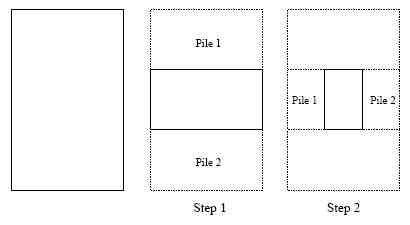
\includegraphics{TeXGraphics/Chapter8Fig.jpg}
	\caption{Tearing paper into thirds to make two piles.}
	\label{ThirdEqualHalf}
\end{figure}

\item Consider Zeno's paradox (refer to the text for details).  Assume that it takes a runner $\frac{1}{2}$ hour to run the first $\frac{1}{2}$
 of the course.  How long would it take the runner to complete the course?  Describe a situation, in the context of the paradox, in which it would take the runner an infinite amount of time to complete the course.

\item Figure \ref{GeoSeries1} gives an informal proof that $
\displaystyle\sum\limits_{n = 1}^\infty  {\frac{1}{{2^n }}}  = 1$.  Explain what is going on.

\begin{figure}[ht]
	\centering
		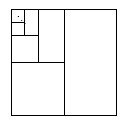
\includegraphics{TeXGraphics/GeoSeries1.jpg}
	\caption{$\displaystyle\sum\limits_{n = 1}^\infty  {\frac{1}{{2^n }}}  = 1$}
	\label{GeoSeries1}
\end{figure}

\item Figure \ref{GeoSeries2} gives an informal proof that $\displaystyle\sum\limits_{n = 1}^\infty  {\frac{3}{{4^n }}}  = 1$.  Explain what is going on. %insert file GeoSeries2.bmp or whatever at this point%
\begin{figure}[ht]
	\centering
		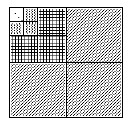
\includegraphics{TeXGraphics/GeoSeries2.jpg}
	\caption{$\displaystyle\sum\limits_{n = 1}^\infty  {\frac{3}{{4^n }}}  = 1$}
	\label{GeoSeries2}
\end{figure}

\end{enumerate}
\section{$p$-series}
\begin{enumerate}

\item If there were something called a $p$-sequence, what would it be?  Compare and contrast the convergence of $p$-series and $p$-sequences.

\item What is a $p$-series?  When do $p$-series converge and when do they diverge?  What tests can we use to verify these results?  

\item If there were something called a $p$-sequence, what would it be?  If there were something called an alternating $p$-series, what would it be?  Compare and contrast the convergence of $p$-series, alternating $p$-series, $p$-sequences and alternating $p$-sequences.

\item Compare and contrast the $p$-series and the $q$-log series.

\end{enumerate}
\section{Integral Test}
\begin{enumerate}

\item Consider the integral test?  How do we apply it?  Using a picture, illustrate why the integral test might be reasonable.  Discuss the difference of the area under a continuous function versus the sum of a discrete set of numbers.

\item Suppose you have (correctly) applied the integral test to the series $
S = \displaystyle\sum\limits_{k = 1}^\infty  {a_k } $ using the function $y = f(x)$ such that $a_n = f(n)$ and you found that $S$ converges.  Does $S = \int_1^\infty  {f(x)\,dx} $?

\end{enumerate}
\section{Comparison Tests}
\begin{enumerate}
\item Suppose $
\displaystyle\sum\limits_{n = 1}^\infty  {a_n }  = L$ and $\displaystyle\sum\limits_{n = 1}^\infty  {b_n }  = K$ where $L < K$.  Is it true that $a_n  \le b_n $ for all $n$?

\item Using the ideas of areas, illustrate and explain how the comparison test works.

\item Compare and contrast the comparison test and the limit comparison test.

\item The comparison test applied to $\displaystyle\sum\limits_{n = 1}^\infty  {a_n } $ and $\displaystyle\sum\limits_{n = 1}^\infty  {b_n } $ where $a_n  \le b_n $ is inconclusive in certain cases.  Illustrate this by finding aseries $\displaystyle\sum\limits_{n = 1}^\infty  {a_n } $ that converges and a series $\displaystyle\sum\limits_{n = 1}^\infty  {b_n } $ that diverges.  Explain why they shows that the direct comparison test can be inconclusive.

\item In the Limit Comparison Test, if $
\mathop {\lim }\limits_{k \to \infty } \frac{{a_k }}{{b_k }} = 0$ and $\displaystyle\sum\limits_{k = 1}^\infty  {a_k } $ converges, explain why the Limit Comparison Test is inconclusive.  \cite{SM}

\item Prove that the limit comparison test applied to $
\displaystyle\sum\limits_{n = 1}^\infty  {a_n } $ and $
\displaystyle\sum\limits_{n = 1}^\infty  {b_n } $
 is inconclusive when $
\mathop {\lim }\limits_{x \to \infty } \frac{{a_n }}{{b_n }} = 0$
 by finding the following examples.
\begin{enumerate}
\item $\mathop {\lim }\limits_{x \to \infty } \frac{{a_n }}{{b_n }} = 0$ for $\displaystyle\sum\limits_{n = 1}^\infty  {a_n } $ and $\displaystyle\sum\limits_{n = 1}^\infty  {b_n } $ that both converge

\item $\mathop {\lim }\limits_{x \to \infty } \frac{{a_n }}{{b_n }} = 0$ and one of $
\displaystyle\sum\limits_{n = 1}^\infty  {a_n } $ and $
\displaystyle\sum\limits_{n = 1}^\infty  {b_n } $ converges and the other diverges


\item Was $\displaystyle\sum\limits_{n = 1}^\infty  {a_n } $ or $\displaystyle\sum\limits_{n = 1}^\infty  {b_n } $ the convergent series?  Do you  think the limit comparison test is inconclusivewhen $\mathop {\lim }\limits_{x \to \infty } \frac{{a_n }}{{b_n }} = 0$?\end{enumerate}

\item Do a direct comparison of each of the following series to the $p$-series with $p = 3$.  Discuss the results of the direct comparison test.  For the comparisons that are not conclusive, what would you try next?$$\displaystyle\sum\limits_{k = 1}^\infty  {\frac{1}{{k^3  - 5k}}} $$	$$\displaystyle\sum\limits_{k = 1}^\infty  {\frac{1}{{k^3  + 5}}} $$	$$\displaystyle\sum\limits_{k = 1}^\infty  {\frac{{k^2  - 3}}{{k^5  + 5k^2 }}} $$


\item Do a direct comparison of each of the following series to the harmonic series.  Discuss the results of the direct comparison test.  For the comparisons that are not conclusive, what would you try next?$$
\displaystyle\sum\limits_{k = 1}^\infty  {\frac{1}{{k - 5}}} $$	$$
\displaystyle\sum\limits_{k = 1}^\infty  {\frac{1}{{k + 1}}} $$	$$
\displaystyle\sum\limits_{k = 1}^\infty  {\frac{{k^2  - 3}}{{k^3  + 5k^2 }}} $$


\end{enumerate}
\section{Root and Ratio Tests}
\begin{enumerate}

\item In the Ratio Test, if $
\mathop {\lim }\limits_{k \to \infty } \left| {\frac{{a_{k + 1} }}{{a_k }}} \right| > 1$, which is "bigger", $\left| {a_{k + 1} } \right|$ or $\left| {a_k } \right|$?  Explain why this implies that the series $\displaystyle\sum\limits_{k = 1}^\infty  {a_k } $ diverges.  \cite{SM}

\item Prove that theratio test is inconclusive for $
\displaystyle\sum\limits_{n = 1}^\infty  {a_n } $ if $\mathop {\lim }\limits_{x \to \infty } \left| {\frac{{a_{n + 1} }}{{a_n }}} \right| = 1$ by finding each of these examples: 
\begin{enumerate}
\item Find $\displaystyle\sum\limits_{n = 1}^\infty  {a_n } $ such that $\displaystyle\sum\limits_{n = 1}^\infty  {a_n } $ converges and $
\mathop {\lim }\limits_{x \to \infty } \left| {\frac{{a_{n + 1} }}{{a_n }}} \right| = 1$.  \item Find $\displaystyle\sum\limits_{n = 1}^\infty  {a_n } 
$ such that $
\displaystyle\sum\limits_{n = 1}^\infty  {a_n } $ diverges and $
\mathop {\lim }\limits_{x \to \infty } \left| {\frac{{a_{n + 1} }}{{a_n }}} \right| = 1$.
\end{enumerate}

\item Prove that the root test is inconclusive for $
\displaystyle\sum\limits_{n = 1}^\infty  {a_n } $ if $\mathop {\lim }\limits_{x \to \infty } \sqrt {\left| {a_n } \right|}  = 1$
 by finding each of these examples:
\begin{enumerate} 
\item Find $\displaystyle\sum\limits_{n = 1}^\infty  {a_n } $ such that $
\displaystyle\sum\limits_{n = 1}^\infty  {a_n } $ converges and $
\mathop {\lim }\limits_{x \to \infty } \sqrt {\left| {a_n } \right|}  = 1$.
\item Find $\displaystyle\sum\limits_{n = 1}^\infty  {a_n } $
such that $\displaystyle\sum\limits_{n = 1}^\infty  {a_n } 
$ diverges and $\mathop {\lim }\limits_{x \to \infty } \sqrt {\left| {a_n } \right|}  = 1$. 
\end{enumerate}

\item Choose a geometric series that converges and one that diverges.  Apply the ratio test to these series.  What is always true about the ratio of a geometric series?  (Check this with the general form.)  Is the ratio test always conclusive for a geometric series?  How are geometric series related to series that one can apply the ratio test to?

\item Describe the characteristics of the terms of a series that you might consider trying the ratio test on.  

\item Compare and contrast the root and ratio test.

\item Describe the characteristics of the terms of a series that you might consider trying the root test on.

\end{enumerate}
\section{Alternating Series}
\begin{enumerate}

\item Can you apply the Alternating Series Test to all series with alternating signs?  Explain.

\item Investigate the validity of this statement:  $
1 - 1 + 1 - 1 + 1 - 1 +  \cdots  = 0$.

\item Determine whether the following series converges or not?  $1 + \frac{1}{2} - \frac{1}{3} - \frac{1}{4} + \frac{1}{5} + \frac{1}{6} -  \cdots $


\item True or false: If $\displaystyle\sum\limits_{n = n_0 }^\infty  {a_n } $
 and converges, then $\displaystyle\sum\limits_{n = n_0 }^\infty  {\left( { - 1} \right)^n a_n } $ converges.

\item True or false: If $\displaystyle\sum\limits_{n = n_0 }^\infty  {\left( { - 1} \right)^n a_n } $  and converges, then $\displaystyle\sum\limits_{n = n_0 }^\infty  {a_n } 
$ converges.

\item What is an alternating series?  Which tests apply to these series and which tests do not?  Why do we have to treat these series differently?

\item Compare and contrast absolute and conditional convergence.

\item What conditions must be satisfied to apply the alternating series test?  Give examples to show that the alternating series test can not be used if any of the hypotheses are ignored.

\item Do we have to treat alternating geometric series in a special case?  Explain.

\item The Alternating Series Test was stated for the series $
\displaystyle\sum\limits_{k = 1}^\infty  {\left( { - 1} \right)^{k + 1} a_k } $.  Explain the difference between $\displaystyle\sum\limits_{k = 1}^\infty  {\left( { - 1} \right)^{k + 1} a_k } $  and $\displaystyle\sum\limits_{k = 1}^\infty  {\left( { - 1} \right)^k a_k } $.  If  $
\displaystyle\sum\limits_{k = 1}^\infty  {\left( { - 1} \right)^{k + 1} a_k }  = K$
  for finite K, what do we know about $
\displaystyle\sum\limits_{k = 1}^\infty  {\left( { - 1} \right)^k a_k } $.  If  $
\displaystyle\sum\limits_{k = 1}^\infty  {\left( { - 1} \right)^{k + 1} a_k } 
$  diverges, what do we know about $\displaystyle\sum\limits_{k = 1}^\infty  {\left( { - 1} \right)^k a_k } $.  Explain why we could have stated the theorem using $\displaystyle\sum\limits_{k = 1}^\infty  {\left( { - 1} \right)^k a_k } $ instead.  \cite{SM}

\item Consider the following table.  Are all these options possible?  For each possible option, find an example.  For each impossible option, given an explanation.  What do we call each of these options?


\begin{center}
\begin{tabular}{|c|c|} \hline
$\displaystyle\sum\limits_{n = n_0 }^\infty  {a_n } $ & $ \displaystyle\sum\limits_{n = n_0 }^\infty  {\left| {a_n } \right|} $ \\   \hline
Converges & Converges \\ \hline
Converges & Diverges \\ \hline
Diverges & Converges \\ \hline
Diverges & Diverges \\ \hline
\end{tabular}
\end{center}



\end{enumerate}
\section{Series Tests}
\begin{enumerate}

\item What does it mean for a series convergence test to be inconclusive?  Which tests have this "special" feature?  What does this mean for your process of trying to determine if a series converges or not?

\item Several of the series tests can be inconclusive.  Make a list of these inconclusive results.  Find series that show why these results are inconclusive.  That is, for each inconclusive result, find two series, one that converges and one that diverges.

\item How do you decide which convergence/divergence test to use on a series?  

\item Compare and contrast the Limit Comparison Test and the Ratio Test.

\item Create a concept map of the series convergence and divergence theorems that helps you understand which ones help us do what.  For instance, which ones only tell us divergence?  Which give the sum?  Which are sometimes inconclusive?  Which only apply to series of nonnegative terms?  What other properties can you think of to use in your concept map?

\item Which convergence/divergence tests only apply to series with nonnegative terms?  Why are they limited in that way?  Look at the answer to this question in 2 ways.  What is different about series with negative terms than series with nonnegative terms that will make a difference in the convergence?  How were the convergence/divergence test derived and where does the nonnegative term requirement appear in that derivation.

\item On the upcoming exam you will have to look at a lot of series and decide how to determine their convergence.  Which tests of convergence do you understand the best and least?  Which tests are easier to decide whether to use or not?  Which tests are easy to apply and which are more difficult?  If there were one test that you could improve on between now and the exam, which would you choose and why?

\item Make a list of all the series convergence tests that you know.  Create a scale to evaluate your understanding of each test (give qualitative meaning to the scale). Rate yourself on each test using this scale.  Now, create a scale to evaluate how well you can apply each test (give qualitative meaning to the scale).  Rate yourself on each test using this scale.  Finally, create a scale to evaluate the test on how useful they are (give a qualitative meaning to the scale).  Rate each test using this scale.  Discuss your observations.

\item We have talked before about existence theorems like the Mean Value Theorem that tell us that a value exists but do not tell us what the value is.  Most of the convergence theorems we have studied are existence theorems.  Why?  What is it that these theorems tell us exists and why doesn't it give us a way to find the value.  Which convergence theorems go beyond existence?

\item We need to be careful when applying any of the series tests.  Can we use the Alternating Series Test on $
\frac{1}{3} - \frac{1}{2} + \frac{1}{9} - \frac{1}{4} + \frac{1}{{27}} - \frac{1}{8} +  \cdots  + \frac{1}{{3^n }} - \frac{1}{{2^n }} +  \cdots $?  Determine the convergence of this series.   \cite{FWG}

\item Look back at the homework and writing assignments you have done so far and identify concepts that you feel you know the best.  Identify areas that you need to improve on before the exam.  If you could improve on one concept before the exam, what concept would be the most beneficial to you and why? Which are the trickiest?

\end{enumerate}


 






\chapter{Vectors, Lines and Planes in Space}

\label{sec:VectorsLinesAndPlanesInSpace}


\section{General}

\begin{enumerate}
\item Discuss the relationship between a 3-dimensional vector and a point in space.  \cite{EP}
\item Give an example of a real-world situation described by a triple of real numbers (other than a point in space).  \cite{EP}
\item Explain why open is not the opposite of closed?  Can a set be both open and closed?  Can a set be neither open nor closed?  Take your examples from both the line and the plane.
\item Write up to 5 distinct questions from the material in this chapter that I might ask on an exam about the following information.
$(-2, 3, 0)$ and $(1, 0, -2)$:
\item Write up to 5 distinct questions from the material in this chapter that I might ask on an exam about the following information:
$(-2, 3, 0)$, $(1, 0, -2)$ and $(1, 0, 0)$.
\item Suppose you were asked to provide a graph represented by $x = 3$.  Explain that to do so you need to know the context in which to graph (1-dimension, 2-dimensions or 3-dimensions).  Explain each possible graph and how it depicts all points where $x = 3$.
\item Look back at the homework and writing assignments you have done so far and identify concepts that you feel you know the best.  Identify areas that you need to improve on before the exam.  If you could improve on one concept before the exam, what concept would be the most beneficial to you and why? Which are the trickiest?
\item It is very important to be able to quickly and accurately visualize three-dimensional relationships.  In three dimensions, describe how many lines are perpendicular to the unit vector $\bf{i}$.  Describe all lines that are perpendicular to $\bf{i}$ and pass through the origin.  In three dimensions, describe how many planes are perpendicular to the unit vector $\bf{i}$.  Describe all planes that are perpendicular to $\bf{i}$ and that contain the origin.  \cite{SM}
\end{enumerate}

\section{Parametric Curves}

\begin{enumerate}

\item Compare and contrast curves of the form  $y = f(x)$ and parametric curves of the form $\left\{ {x = x(t),y = y(t)} \right\}$.  In particular, discuss the representations of these curves, the roles of the dependent variable, the independent variable(s) and the parameter, and the value of each representation.
\item Compare and contrast the representations of the same curve as $$y=f(x),$$ $$\left\{ {x = t,y = f(t)} \right\}$$ and $$\left\{ {x = f^{-1}(s),y = s} \right\}.$$
\item Write up to 5 distinct questions from the material in this chapter that I might ask on an exam about the following information:
$$\left\{ \matrix{ x = 3t - 5 \hfill \cr y = t^2  \hfill \cr}  \right\}$$ for $-1 \le t \le 2$.
\item Compare and contrast the graphs of $$\left\{ \matrix{  x = \cos ^2 t \hfill \cr   y = \sin ^2 t \hfill \cr}  \right\}$$ and $x + y = 1$.
\item Consider the parametric curve 
$$\left\{ \matrix{  x = a+r\cos t \hfill \cr   y = b+r\sin t \hfill \cr}  \right\}.$$  Describe as completely and as generally as possible the shape and orientation of this curve.  Describe how the curve is drawn out as $t$ ranges from 0 to $2\pi$.  Find a nonparametric representation of this curve.
\item  Consider the parametric curve 
$$\left\{ \matrix{  x = a+r t \hfill \cr   y = b+r t \hfill \cr}  \right\}$$
 for $0\le t\le t_1$.  Describe as completely and as generally as possible the shape and orientation of this curve.  Describe how the curve is drawn out as $t$ ranges from 0 to $t_1$.  Find a nonparametric representation of this curve.
\end{enumerate}

\section{Lines and Planes}

\begin{enumerate}

\item Compare and contrast the parametric and symmetric forms of the equation of a line in three dimensions.
\item Compare and contrast finding equations of lines in 2-space and in 3-space.
\item What do we need to know to find the equation of a line in 3-space?  Give as many different ways that information can be given to us.
\item Compare and contrast finding equations of lines in 2-space and equations of planes in 3-space.
\item Compare and contrast finding equations of lines in 3-space and equations of planes in 3-space.
\item Compare and contrast finding intersections of lines in 2-space and finding intersections of lines in 3-space.
\item How do we analytically describe a line in 3-space?  Why do we have to describe it that way?  Why can we not describe a line with a single equation?
\item Explain how to find the intersection and orientation of 2 lines in 3-space.  Detail the possible orientations.
\item Detail the possible orientations of a line and a plane in 3-space.  Explain how to determine which of those possible orientations a line and plane actually have.
\item Detail the possible orientations of 2 planes in 3-space.  If 2 planes intersect, what is the resulting intersection?  
\item Write up to 5 distinct questions from the material in this chapter that I might ask on an exam about the following information:
$$\left\{ \matrix{  x = 3 + 2t \hfill \cr   y = 2 - t \hfill \cr  z = 5 + t \hfill \cr}  \right\}$$ and $$\left\{ \matrix{  x =  - 3 - s \hfill \cr  y = 7 + s \hfill \cr  z = 16 + 3s \hfill \cr}  \right\}.$$
\item Write up to 5 distinct questions from the material in this chapter that I might ask on an exam about the following information.
$3x- 2y + z- 1 = 0$ and $2z + 3 = 0$.
\item Does it make sense to talk about the $x$-, $y$-, and $z$-intercepts of $$\left\{ \matrix{  x = 1 + 2t \hfill \cr   y =  - 1 - t \hfill \cr   z = 3t \hfill \cr}  \right\}?$$  Describe the method of finding where this line intersects each of the coordinate planes.  \cite{FWG}
\item Consider the planes of the form $${x \over a} + {y \over b} + {z \over c} = 1.$$  What do these planes look like in general and what do the values of a, b, and c represent?   (Hint:  Think about the lines of the form $${x \over a} + {y \over b} = 1$$ and try to generalize.)
\item Consider the plane $2x + y - z = 8$ and the line $$\left\{ {x = 1 - 2t,\;y = 2 + 5t,\;z =  - 3t} \right\}.$$  Explain how to determine the orientation of these two objects, i.e., are they parallel or do they intersect and, if they intersect, are they perpendicular?  \cite{FWG}
\item Explain how to find equations of 2 distinct planes that intersect along the line $$\left\{ \matrix{  x = 1 + t \hfill \cr y = 2 - t \hfill \cr  z = 3 + 2t \hfill \cr}  \right\}.\ \cite{FWG}$$  
\item 

\begin{enumerate} 
\item Explain how to create two different sets of parametric equations of lines that are coincident. 
\item Explain how to create two sets of parametric equations of lines that are parallel but not coincident. 
\item Explain how to create sets of parametric equations of lines that are skew. 
\item Explain how to create sets of parametric equations of lines that intersect and are perpendicular. 
\end{enumerate}

\item What is the relationship between the angle between 2 planes and the angle between the normal vectors of those planes.  Create a physical model to help illustrate this to another student.
\item How can you look at the equation of a plane and decide that it is parallel to the $x$-axis?  Generalize.
\item You and a friend were comparing homework and you got different answers to 
this question:  Find the parametric equation of the line passing through the two points $(1, 2, 2)$ 
and $(3, -1, 3)$.  $$\rm{Your}\ \rm{ answer}  \left\{ \matrix{  x = 1 + 2t \cr   y = 2 - 3t \cr   z = 2 + t \cr}  
\right\}$$$$\rm{Your}\  \rm{friend's}\ \rm{answer}\left\{ \matrix{  x =  - 2s + 3 \cr   y = 3s - 1 \cr   z =  - s + 3 \cr}  \right\}$$  Should either, both or neither of you be worried?
\item Explain how to shift back and forth between the parametric and symmetric equations of the line.  Describe one situation in which you would prefer to have parametric equations to work with and one situation in which symmetric equations would be more convenient.  \cite{SM}
\item Notice that if $c = 0$ in the general equation $ax + by + cz + d = 0$ of a plane, you have an equation that would describe a line in the $xy$-plane.  Describe how the line $ax + by + d = 0$ in the $xy$-plane relates to the plane $ax + by + d = 0$.  \cite{SM}
\end{enumerate}

\section{Vectors, Projections and Vector Products}

\begin{enumerate}

\item Compare and contrast the concepts of points in the plane and vectors in the plane. 
\item Describe how the formula for distance in 2-space is derived from the Pythagorean theorem.  Explain how to find distance in 3-space.
\item Compare and contrast the dot product and cross product including a discussion of properties and uses of the two products.
\item If $\bf{u}$, $\bf{v}$, and $\bf{w}$ are coplanar, explain why $$\bf{u} \cdot \left( {\bf{v} \times \bf{w}} \right) = 0$$ and $$\left( {\bf{u} \times \bf{v}} \right) \cdot \bf{w} = 0.$$
 \item A friend of yours missed class the day we talked about vectors for the first time.  Explain to your friend what a scalar is and how it is different than a vector.  How do you find a vector's magnitude and direction?
 \item If a vector is multiplied by a positive scalar, how is the result related to the original vector?  What if the scalar is zero?  Negative? \cite{FWG}  Less than 1?  Greater than 1?
 \item What is the dot product?  How is it calculated?  How do we interpret the dot product?  When is the dot product of two vectors equal to zero?
 \item Describe and illustrate the vector projection of a vector $\bf{u}$ onto a vector $\bf{v}$.  Give several distinct examples.
 \item What is the cross product?  How is it calculated?  How do we interpret the cross product?  When is the cross product of two vectors equal to zero?
 \item Suppose that vectors ${\bf{u}}$, ${\bf{v}}$ and ${\bf{w}}$ are coplanar, that is, if ${\bf{u}}$, ${\bf{v}}$ and ${\bf{w}}$ were positioned so they share the same inital point, then all 3 vectors would lie in the same plan.  Use a geometric argument to prove that $$
{\bf{u}} \cdot \left( {{\bf{v}} \times {\bf{w}}} \right) = 0
$$
and $$
\left( {{\bf{u}} \times {\bf{v}}} \right) \cdot {\bf{w}} = 0
.$$

 \item Write up to 5 distinct questions from the material in this chapter that I might ask on an exam about the following information:$\bf{u} = 3{\bf{i}} + 2{\bf{j}}$ and $\bf{v}= -{\bf{j}}.$
 \item Compare and contrast the usage of the words perpendicular, orthogonal and normal.
 \item What is the "right-hand rule" and what does it help us visualize?  If there were a "left-hand rule" what would it help us visualize?
 \item 
 \begin{enumerate} 
 \item Find the area of the triangle determined by the points $(1, 2, 0)$, $(-1, 2, 0)$ and $(0, 0, 0)$ using a cross product. 
 \item Check your answer to the first part of this question by finding the area using the formula $A = 0.5 bh$. 
 \item Explain why the process in the first part of this questionis useful (i.e., why would we use the cross product instead of the formula $A = 0.5 bh$?)
 \end{enumerate}
 \item We know that if $$\bf{u} \times \bf{v} = 0,$$ then $\bf{u}$ and $\bf{v}$ are parallel.  Why is this true?  Why is this not an efficient method for determining if 2 given vectors are parallel?
 \item Explain how to determine if $\bf{u} = \left\langle  a, b \right\rangle $ and $\bf{v} = \left\langle c, d\right\rangle $ are orthogonal by inspection.  Explain why we cannot decide if $\bf{u} = \left\langle a, b, c\right\rangle$ and $\bf{v} = \left\langle d, c, e\right\rangle$ are orthogonal by inspection.
 \item What is the relationship between $${\bf{a}} \cdot {\bf{b}}$$ and $${\bf{b}} \cdot {\bf{a}}?$$  What is the relationship between $${\bf{a}} \times {\bf{b}}$$ and $${\bf{b}} \times {\bf{a}}?$$  Be sure to use geometry as part of your explanation.
 \item Compare and contrast $${{\left| {{\bf{a}} \cdot {\bf{b}}} \right|} \over {\left| {\bf{a}} \right|\left| {\bf{b}} \right|}}$$and $${{\left| {{\bf{a}} \times {\bf{b}}} \right|} \over {\left| {\bf{a}} \right|\left| {\bf{b}} \right|}}.$$
 \item What is $$\vec 0 \cdot \left( {a\hat i + b\hat j + c\hat k} \right)?$$  How should we interpret this result?  
 \item If $(a, b)$ and $$\left\langle {a,b} \right\rangle  = a\hat i + b\hat j$$ are both represented by an ordered pair of numbers, why can we talk about the length of $$\left\langle {a,b} \right\rangle $$ but not $(a, b)$?
 \item Compare and contrast scalar multiplication (a)(b) and the dot product $$\bf{u} \cdot \bf{v}.$$
 \item Compare and contrast scalar multiplication $(a)(b)$ and the cross product $$\bf{u} \times \bf{v}.$$
 \item Show that except in degenerate cases, $$\left( {\bf{u} \times \bf{v}} \right) \times \bf{w}$$ lies in the plane of $\bf{u}$ and $\bf{v}$ whereas $$\bf{u} \times \left( {\bf{v} \times \bf{w}} \right)$$ lies in the plane of $\bf{v}$ and $\bf{w}$.  Describe the degenerate cases.  \cite{FWG}
 \item Prove that $$\left| {\bf{u} \cdot \bf{v}} \right| \le \left\| \bf{u} \right\|\,\left\| \bf{v} \right\|.$$ Under what circumstance is $$\left| {\bf{u} \cdot \bf{v}} \right| = \left\| \bf{u} \right\|\,\left\| \bf{v} \right\|? \cite{FWG}$$  
 \item A river 2.1 miles wide flows south with a current of 3.1 miles per hour.  What speed and heading should a motorboat assume to travel across the river from east to west in 30 minutes?  \cite{SBS}
 \item If $\bf{u}$ and $\bf{v}$ are nonzero vectors and $$\left\| \bf{u} \right\| = \left\| \bf{v} \right\|,$$ does it follow that $\bf{u}=\bf{v}$?  \cite{SBS}
 \item What is the standard basis of vectors in ${\Re}^3 $?  What purpose does the bases serve?
 
 \item Assume that $\bf{u}$ and $\bf{v}$ are 2-dimensional vectors.  Which of the following operations are not defined and why?  If the operation is defined, is the result scalar or vector? 
 
 \begin{center}
 \begin{tabular}{l}
 $\bf{u} \cdot \bf{v}$\\ 
 $\bf{u} \times \bf{v}$\\
 $\bf{u} \cdot \left( {\bf{v} \cdot \bf{w}} \right)$\\ 
 $\bf{u} \times \left( {\bf{v} \times \bf{w}} \right)$\\ 
 $\bf{u} \cdot \left( {\bf{v} \times \bf{w}} \right)$\\
 $\bf{u} \times \left( {\bf{v} \cdot \bf{w}} \right)$\\ 
 \end{tabular} 
 \end{center}
 
 Repeat this exercise assuming that u and v are 3-dimensional vectors.  Discuss.
 
 \item Briefly describe each of the following processes:  how to determine if 2 vectors are parallel, how to determine if 2 vectors are perpendicular, how to determine if 3 points are collinear, andhow to determine if 4 points are coplanar.  \cite{SM}
 \item Briefly describe how to construct a vector parallel to a given vector.  Briefly describe how to construct a vector perpendicular to a given vector.  Given a vector, describe how to construct 2 other vectors such that the three vectors are mutually perpendicular.  \cite{SM}
 
 \item Consider 2 3-dimensional vectors $\bf{u}$ and $\bf{v}$.  Describe the results of each of the following vector expressions in words and with a diagram where possible.
 
 \begin{center}
 \begin{tabular}{l}
 $3\bf{v}$\\ 
 $-3\bf{v}$\\
 
  $\left\| \bf{u}\right\| + \left\| \bf{v}\right\|$\\ 
  $\bf{u} \cdot \bf{v}$\\
  $\bf{v} \cdot \bf{u}$\\
  $\bf{v} \cdot \bf{v}$\\
 $\bf{u} \times \bf{v}$\\
 $\bf{v} \times \bf{u}$\\
  $\bf{v} \times \bf{v}$\\
	${{\bf{v}} \over \left\| {\bf{v}} \right\|}$\\ 
  \end{tabular} 
 \end{center}
 

\end{enumerate}

\section{General Surfaces}

\begin{enumerate}

 \item Compare and contrast finding equations of circles in 2-space and spheres in 3-space.
 \item In space why do we refer to the surfaces like $x^2 - y = 0$ as a cylinder.  Explain the geometry of this and related surfaces.  How do we distinguish cylinders from other surfaces?  How do we graph cylinders?
\end{enumerate}




\chapter{Vector Valued Functions}

These questions are sorted into the categories  1) general, 2) vector functions, 3) curvature, 4) derivatives and tangent lines and 5) area and arc length.

\section{General}\begin{enumerate}

\item Write up to 5 distinct questions from the material in this chapter that I might ask on an exam about the following information.
$$\left\{ \matrix{  x = \sin t \hfill \cr   y = \cos t \hfill \cr   z = t \hfill \cr}  \right\}$$

\item We have now seen three different ways to represent a curve in the plane:  $y = f(x)$, 
$r = r(\theta)$, and $$\left\{ \matrix{  x = x(t) \hfill \cr   y = y(t) \hfill \cr}  \right\}.$$  What are the advantages and disadvantages of each representation?  Describe an application you would use each representation for and explain your choices.

\item Look back at the homework and writing assignments you have done so far and identify concepts that you feel you know the best.  Identify areas that you need to improve on before the exam.  If you could improve on one concept before the exam, what concept would be the most beneficial to you and why? Which are the trickiest?

\end{enumerate}\section{Vector Functions and Parametric Curves}\begin{enumerate}



\item What curve is described by the following equations?  What happens if we tweak $a$, $b$ and $c$?
$$\left\{ \matrix{  x(t) = a\sin t \hfill \cr   y(t) = b\cos t \hfill \cr   z(t) = ct \hfill \cr}  \right\}$$

\item Compare and contrast the graphs of the following.
$$\left\{ \matrix{  x\left( t \right) = \cos t \hfill \cr   y(t) = \sin t \hfill \cr}  \right\}\ \rm{for}\ t   \in   [0, 2 ]$$   $$\left\{ \matrix{  x\left( t \right) = \sin t \hfill \cr   y(t) = \cos t \hfill \cr}  \right\}\ \rm{for}\ t  \in [0, 2 ]$$  $$\left\{ \matrix{  x(t) = {{1 - t^2 } \over {1 + t^2 }} \hfill \cr   y(t) = {{2t} \over {1 + t^2 }} \hfill \cr}  \right\}\ \rm{for}\ t    \in  [-20, 20]$$

\item Suppose that ${\bf{r}}(t) = f(t){\bf{i}} + g(t){\bf{j}} + h(t){{\bf{k}}}$, where $$\mathop {\lim }\limits_{x \to 0} f(t) = \mathop {\lim }\limits_{x \to 0} g(t) = 0$$ and $$\mathop {\lim }\limits_{x \to 0} h(t) = \infty .$$  Describe what is happening graphically as $t \rightarrow 0$ and explain why $$\mathop {\lim }\limits_{x \to 0} {{\bf{r}}}(t)$$ does not exist.  \cite{SM}

\item Suppose that ${\bf{r}}(t)$ is a vector-valued function such that ${{\bf{r}}}(0) = a{\bf{i}} + b{\bf{j}} + c{\bf{k}}$ and $${\bf{r'}}(0)$$ exists.  Imagine zooming in on the curve traced out by ${\bf{r}}(t)$ near the point $(a, b, c)$.  Describe what the curve will look like and how it relates to the tangent vector $${\bf{r'}}(0).\ \cite{SM}$$  

\item Suppose that 2 missiles are fired and both missiles are flying in the same plane.  Assume that the path of the 2 missiles are given by the parametric equations $$\left\{ \matrix{  x_1 (t) \hfill \cr   y_1 (t) \hfill \cr}  \right\}$$ (first missile) and $$\left\{ \matrix{  x_2 (t) \hfill \cr   y_2 (t) \hfill \cr}  \right\}$$ (second missile). Explain the difference between the 2 missiles colliding and the paths of the 2 missiles crossing with no collision.  
	Let the path of the first missile be given by $$\left\{ \matrix{  x_1 (t) = 100t \hfill \cr   y_1 (t) = 80t - 16t^2  \hfill \cr}  \right\}$$ for $0 \le t \le 5$ seconds and the path of the second missile be given by $$\left\{ \matrix{  x_2 (t) = 500 - 200\left( {t - 2} \right) \hfill \cr   y_2 (t) = 80\left( {t - 2} \right) - 16\left( {t - 2} \right)^2  \hfill \cr}  \right\}$$ for 
$2 \le t \le 7$ seconds (the second missile was shot off 2 seconds later than the other missile.)  Explain how to determine if the paths of the missiles cross and how to determine if the missiles collide.

\item Graph $$\left\{ \matrix{  x(t) = \cos t \hfill \cr   y(t) = \sin t \hfill \cr}  \right\}.$$  What should the graph look like?  The graph probably looks like an ellipse.  How do you fix the display so that the graph looks "right"?

\item You have probably seen the turntables on which luggage rotates at the airport.  Suppose that such a turntable has two long straight parts with semicircles on the end.  We will attempt to model the motion of someone's luggage that has not been retrieved from the turntable.  We focus on the left/right movement of the luggage.  Suppose the straight part is 40 feet long, extending from $x = -20$ to $x = 20$.  Assume that our luggage starts at time $t = 0$ at location $x = -20$, and it takes 60 seconds for the luggage to reach $x= 20$.  Suppose the radius of the circular motion is 5 feet, and it takes the luggage 30 seconds to complete the half-circle.  We model the straight-line motion with a linear function $x(t) = at + b$.  Find constants $a$ and $b$ so that $x(0) = -20$ and $x(60) = 20$.  For the circular motion, we use a cosine (Why is this a good choice?) $x(t) = 20 + d \cos (et + f)$ for constants $d$, $e$ and $f$ to make this work.  Find equations for the position of the luggage along the backstretch and the other semicircle.  What would the motion be from then on?    \cite{SM}

\item Explain how to parameterize the line from $(2, 3)$ to $(-4, 8)$ such that at $t = 0$ you are at the former point and at $t = 1$ you are at the latter point.  Generalize.

\item Compare and contrast the curve defined parametrically by $$\left\{ \matrix{  x = f(t) \hfill \cr   y = g(t) \hfill \cr}  \right\}$$ and the curve traces out by the terminal point of the vector-valued function ${\bf{r}}(t) = f(t)i + g(t){\bf{j}}$.  

\item Compare and contrast the graphs of ${\bf{r}}(t) = (2t - 1){\bf{i}} + (t^2){\bf{j}} + t{\bf{k}}$, 
$s(t) = (2 \sin t - 1){\bf{i}} + (\sin 2 t){\bf{j}} + (\sin t){\bf{k}}$, and $u(t) = (2e^t - 1){\bf{i}} + (e^{2t}){\bf{j}} + e^{t}{\bf{k}}$. \cite{SM}

\item Compare and contrast the terms continuous, differentiable, continuously differentiable and smooth as they apply to vector functions.  What extensions could be made of these concepts?

\item Write up to 5 distinct questions from the material in this chapter that I might ask on an exam about the following information.
${\bf{r}}(t) = t{\bf{i}} + 2t{\bf{j}} +3t{\bf{k}}$ over $[0, 2]$

\item Compare and contrast parametric representations of curves in 3-space with vector representations.

\item "Finding a vector function" and "parameterizing a curve" mean the same thing.  Describe how to do this in two different contexts.  First, in the plane parameterize the curve $y = 3x^3 - 2x$.  In general, describe how to parameterize any function $y = f(x)$.  In the second context, find the vector function who graph is the curve of intersection of the cylinder $z = x^2 + y^2$ and the plane $x + 2y - 3z = 1$ for $x > 0$.

\item What is a vector-valued function?  Explain what it means for a vector-valued function to be continuous.

\item Consider any vector-valued function in the plane whose path is a line.  Do the components of the function have to be linear?  Answer by either proving they have to be linear or demonstrating that they do not.  If they do not have to be linear, for what reason might we want the components to not be linear?

\item Practically everything you can do to combine $y = f(x)$ and $y = g(x)$ results in another function of one variable.  This is not true of vector-valued functions in space.  Make a list of operations that can be performed on ${\bf{F}}(t)$ and ${\bf{G}}(t)$, how these operations are performed, and which result in vector-valued functions and which do not (and why not).

\end{enumerate}\section{Curvature}\begin{enumerate}


\item Throughout our study of calculus, we have looked at tangent line approximations to curves.  Some tangent lines approximate a curve well over a fairly lengthy interval while some stay close to a curve for only very short intervals.  Explain how you can use curvature to predict whether a curve will be well approximated by its tangent line.  \cite{SM}

\item Explain what it means for a curve to have zero curvature at a point. Explain what it means for a curve to have zero curvature on an interval.  \cite{SM}

\item True or false:  The curvature of the 2-dimensional curve $y = f(x)$ is the same as the curvature of the 3-dimensional curve ${{\bf{r}}}(t) = t{\bf{i}} + f(t){\bf{j}} + c{\bf{k}}$ where $c$ is a constant.  \cite{SM}

\item True or false:  The curvature of the 2-dimensional curve $y = f(x)$ is the same as the curvature of the 3-dimensional curve ${\bf{r}}(t) = t{\bf{i}} + f(t){\bf{j}} + t{\bf{k}}$.  \cite{SM}

\item Discuss the relationship between curvature and concavity for the function $y = f(x)$. \cite{SM}

\item What is curvature?  How do we measure it?  How do we visually compare the curvature at 2 different points on a curve?

\item Give an example of a curve where the largest curvature occurs at an extreme point.  Give an example of a curve where the largest curvature occurs at a point that is not an extreme point.

\item Why are we given so many different formulas for curvature?  Discuss the need or convenience of these formulas.

\end{enumerate}\section{Derivatives and Tangent Lines}\begin{enumerate}

\item Compare and contrast a tangent line to a curve at a point and an osculating circle of radius $${1 \over \kappa }$$ at the same point.

\item The derivative $${\bf{F'}}(t)$$ of a vector-valued function ${\bf{F}}(t)$ is another vector-valued function.  What do the vectors we obtain from ${\bf{F}}(t)$ represent?  What does it mean if $${{\bf{F}}}\left( {t_0 } \right) = {\bf{0}}$$? What do the vectors we obtain from $${\bf{F'}}(t)$$ represent?  What does it mean if $${\bf{F'}}\left( {t_0 } \right) = {\bf{0}}?$$

\item Compare and contrast the notions of speed and velocity of a moving object.  \cite{SBS}

\item Consider the parametric curve ${\bf{F}}(t)$, its derivative $${\bf{F'}}(t),$$ its arc length $s(t)$ as a function of $t$, the derivative of the arc length $$s'(t),$$ the modulus $$\left\| {{{\bf{F}}}(t)} \right\|,$$ and the modulus of the derivative $$\left\| {{\bf{F'}}(t)} \right\|.$$  Make a concept map of these objects and describe what each measures.

\item The speedometer on your car reads a steady 35 mph.  Could you be accelerating?  \cite{FWG} 

\item When tracking the motion of an object such as a comet, it is often convenient to think of the object's position as a function of time.  In two dimensions, the object's position would be given by functions $x(t)$ and $y(t)$.  Relatively simple polynomial functions can interact to produce complicated parametric graphs.  Use a calculator to graph $$x(t) = t^2  - 2$$ and $$y(t) = t^3  - t - 1.$$  Find the point $(x, y)$ and the value of $t$ where the loop begins.  Try to explain in terms of the properties of $x(t)$ and $y(t)$ why it loops.  \cite{SM}

\end{enumerate}\section{Area and Arc Length}\begin{enumerate}

\item Explain how the formula for area under a parametric curve,$$\int\limits_a^b {y(t)x'(t)} dt,$$ is derived.

\item What is the formula for finding the length of a segment of a smooth curve in 2-space?  In 3-space?  Explain, in general terms, the derivation of this formula.

\item What is the formula for finding the length of an arc of $$\left\{ \matrix{  x = x(t) \hfill \cr   y = y(t) \hfill \cr}  \right\}?$$  Explain, in general terms, the derivation of this formula.  What hypotheses about the curve must be checked before you apply the formula?  What would you do if the curve did not satisfy these hypotheses?  How would you extend the formula for finding the length of an arc of $$\left\{ \matrix{  x = x(t) \hfill \cr   y = y(t) \hfill \cr   z = z(t) \hfill \cr}  \right\}?$$

\item Compare and contrast the formulas for finding the length of an arc of $y = f(x)$ and $$\left\{ \matrix{  x = x(t) \hfill \cr   y = y(t) \hfill \cr}  \right\}.$$  Why do we not talk about finding the length of an arc of $z = f(x, y)$?

\end{enumerate}



 
\chapter{Partial Derivatives} 

\section{General}\begin{enumerate}

\item  Write up to 5 distinct questions from the material in this chapter that I might ask on an exam about the following information:  $$f(x,y) = x^2  - xy + y^2  - 3.$$

\item  Why is sketching $z = f(x, y)$ on paper problematic?  What sketching alternatives do we have to help us handle the problems involved with sketching $z = f(x, y)$?  What does each of these alternative sketching techniques represent?

\item  In general, what is an independent and dependent variable.  Give a "real" situation where there are 2 (or more!) variables and determine which are dependent and which are independent and why. Discuss the independence and dependence of the variables in the following definitions.
\begin{enumerate}\item$\left\{ \matrix{  r = r(x,y) \hfill \cr   s = s(x,y) \hfill \cr   t = t(x,y) \hfill \cr}  \right\}$	\item $M = M(a,b)$ \item $z = z(a, b, c)$ \end{enumerate}

\item  Compare and contrast finding the domain of $y = f(x)$ and $z = f(x, y)$.

\item  We have seen structures in the plane and in space that are defined by single equations (in 2 or 3 variables) and by parametric equations.  You should be able to identify the type of object (curve or surface) and its home (the plane or space) by the number of variables, parameters and equations.  You should also know when a set of parametric equations could be written as a single equation (assuming the algebra works out nicely).  Identify each of the following as a curve or surface (or neither) and whether it lives in the plane or in space (or neither).  Determine if (given nice algebra) the parametric equations could be written as a single equation.  Explain the process by which you made your determinations.
\begin{enumerate}\item $\left\{ \matrix{  a = a(m) \hfill \cr   b = b(m) \hfill \cr}  \right\}$
\item $M = M(a,b)$ \item $\left\{ \matrix{  r = r(x,y) \hfill \cr   s = s(x,y) \hfill \cr   t = t(x,y) \hfill \cr}  \right\}$
\item  $z = z(a, b, c)$ \item $\left\{ \matrix{  a = a(u) \hfill \cr   b = b(u) \hfill \cr   c = c(u) \hfill \cr}  \right\}$ \item $R = R(m)$ \end{enumerate}

\item  Comment on this statement:  The graph of the function $f$ of 1 variable is the set of all points in the plane with coordinates of the form $(x, f(x))$.  Extend this statement to functions of 2 variables. Extend this statement to functions of 3 variables.

\item  Look back at the homework and writing assignments you have done so far and identify concepts that you feel you know the best.  Identify areas that you need to improve on before the exam.  If you could improve on one concept before the exam, what concept would be the most beneficial to you and why? Which are the trickiest?

\item  Give a real-life example of each of the following  functions: $y = f(x)$, $z = f(x, y)$, $w = f(x, y, z)$ and  $u = f(x, y, z, w)$.

\item  What ``nice'' properties would we expect of $f(x,y) = P(x, y)$ where $P$ is a polynomial in $x$ and $y$? \end{enumerate}\section{Level Curves, Traces and Level Surfaces}\begin{enumerate}

\item  Compare and contrast level curves and level surfaces.

\item  Give several real life examples of contour maps and how the contours on the map are used.  Explain what function of 2 variables is used in each contour map.

\item  What do these words mean and what do they have in common:  contour maps, isoclines, isotherms, isobars, and equipotentials?

\item  Explain level curves and traces of a surface.  How do these curves help you understand the shape of a surface?

\item  Compare and contrast level curves and contour maps.

\item  Consider $f(x,y) = 2 - x - {\textstyle{1 \over 2}}y$.  What is the graph of this function?  What are its key features?  If you were to graph this curve by hand, what would be the best way to do it?  How does that compare to how Maple (or other software) graphs this?  Which do you prefer, your graph or the machine's graph?

\item  Let $z = f(x, y)$ be a polynomial function.  Explain why every level curve of $f$ is a closed curve.  For what type of function would that not be true?

\item  Explain why a contour plot without labels identifying the values of $z$ could correspond to more than one function.  \cite{SM}

\item  If a contour plot shows a set of concentric circles around a point, explain why you would expect that point to be the location of a local extreme.  \cite{SM}  What additional information do you need to determine the nature of the extreme value? Why might it not be an extreme?

 \end{enumerate}\section{Limits}\begin{enumerate}

\item  What does it mean for a function $z = f(x, y)$ to have a limit $L$ as $(x,  y) \rightarrow (x_0, y_0)$? \cite{FWG}   What must be true for this limit to exist and how does this differ from limits of functions of 1 variable?  How do we determine, analytically, that the limit does not exist?  Why is this difficult?  

\item  What does it mean for a function $f(x, y)$ to be continuous?  What might $f(x, y)$ look like at a point of discontinuity?

\item  Investigate the validity of this statement:  If $f(x, y)$ approaches the same value $L$ as $(x, y)$ approach $(a, b)$ along every straight line through the point $(a, b)$, then it follows that $$\mathop {\lim }\limits_{(x,y) \to (a,b)} f(x,y) = L.$$

\item  Investigate the validity of this statement:  A quotient of 2 functions $f(x, y)$ and $g(x, y)$ is continuous wherever both of these functions are continuous.

\item  I am looking at $$\mathop {\lim }\limits_{(x,y) \to (0.0)} f(x,y)$$ and I have found that 
$$\mathop {\lim }\limits_{(x,0) \to (0.0)} f(x,y) = A,$$  $$\mathop {\lim }\limits_{(0,y) \to (0.0)} f(x,y) = A,$$ $$\mathop {\lim }\limits_{(x,x) \to (0.0)} f(x,y) = A,$$ and $$\mathop {\lim }\limits_{(x, - x) \to (0.0)} f(x,y) = A.$$  
Explain what each of these limits represents.  Can I safely assume that $$\mathop {\lim }\limits_{(x,y) \to (0.0)} f(x,y) = A?$$

\item  Recall that a function of one variable $y = f(x)$ is continuous at $x = a$ if  $$\mathop {\lim }\limits_{x \to a} f(x)$$ exists,  $f(a)$ exists, and  $$\mathop {\lim }\limits_{x \to a} f(x) = f(a).$$  We also discussed the ways in which a function might not satisfy each part of the definition.  Extend this definition to functions of 2 variables.  Discuss ways in which functions of 2 variables might not satisfy the definition of continuity. 

\end{enumerate}\section{Slopes, Tangent Planes and Partial Derivatives}\begin{enumerate}

\item  Discuss the various slopes associated with a specific point on a surface.  How are these slopes calculated?  How are these slopes used?

\item  How are the partial derivatives $${{\partial f} \over {\partial x}}$$ and $${{\partial f} \over {\partial y}}$$ defined?  How are they interpreted and calculated?  \cite{FWG}

\item  How does the relationship between first partial derivatives and continuity of functions of 2 variables compare and contrast to the relationship between first derivatives and continuity for function of a single variable?  \cite{FWG}

\item  What does it mean for a function $f(x, y)$ to be differentiable?  What might $f(x, y)$ look like at a point where it was not differentiable?

\item  How can you sometimes decide from examining $f_x$ and $f_y$ that a function $f(x,y)$ is differentiable?  \cite{FWG}

\item  What is the relation between the differentiability of $f(x,y)$ and the continuity of $f(x,y)$ at a point?  \cite{FWG}

\item  What is a directional derivative?  How is it calculated and how it is interpreted?  Why do functions of 1 variable not have separate directional derivatives, while functions of 2 variables do?

\item  What rates do $f_x$ and $f_y$ measure?  What rate does a directional derivative in the direction of ${\bf{u}}$ measure?

\item  At the point (1, 2) the function $f(x,y)$ has a derivative of 2 in the direction toward (2, 2) and a derivative of $-2$ in the direction toward (1,1).  Find $f_x(1, 2)$ and $f_y(1, 2)$.  Find the derivative of $f$ at (1, 2) in the direction toward the point (4, 6).  \cite{FWG}

\item  How do we measure sensitivity to change in a function?  Near the point (1, 2) is $$f(x,y) = x^2  - xy + y^2  - 3$$ more sensitive to changes in x or in changes in $y$?  Illustrate what this means with a diagram of what $f(x,y)$ looks like near (1, 2).

\item  If we are given a total differential for a function of 2 variables we can recover the original function $f(x, y)$.  Find a function $f(x,y)$ such that $$df = \left( {ye^{xy}  + 3x^2 } \right)dx + \left( {xe^{xy}  - \cos y} \right)dy.$$  However, not every expression of the form 
$P(x, y)dx + Q(x, y)dy$ is a total differential of some function.  Show that there is no function $f(x,y)$ for which $$\left( {3x + 2y} \right)dx + x\,dy$$ is the total differential.

\item  Suppose a bug is sitting at a specific point on a metal plate and the temperature at a point $(x, y)$ on the plate is give by a differentiable function $T(x, y)$.  Let u be the vector that gives the direction the bug should move in order to cool off as fast as possible. Let v be the vector that gives the direction the bug should move in order to warm up as fast as possible.  Explain why ${\bf{u}} = -{\bf{v}}$.  In other words, why can't the angle between u and v be something other than $\pi$?  
	What if we forget to require $T(x, y)$ to be differentiable?  Now, can we create a function such that the angle between ${\bf{u}}$ and ${\bf{v}}$ be something other than $\pi$?  If so, find such a function.  If not, explain why not.

\item  At one point in the text they claim that the tangent plane to the surface $z = f(x,y)$ at 
$(a, b, f(a, b)) is z = f_x(a, b)(x - a) + f_y(a, b)(x - b) + f(a, b)$.  At another point they say that the tangent plane to the surface defined by $F(x, y, z) = 0$ at $$\left( {x_0 ,y_0 ,z_0 } \right)$$ is $$\bar \nabla f\left( {x_0 ,y_0 ,z_0 } \right) \cdot \left[ {\left( {x,y,z} \right) - \left( {x_0 ,y_0 ,z_0 } \right)} \right] = 0.$$  Are these the same?

\item  Consider the function $z = f(x, y)$. Explain and illustrate the meaning and application of this mathematical statement:  $$df = f_x \left( {a,b} \right)\,\Delta x + f_y \left( {a,b} \right)\,\Delta y.$$

\item  Compare and contrast the differential $$dy = f'\left( x \right)dx$$ for $f(x)$ to the total differential $$dz = {{\partial g} \over {\partial x}}dx + {{\partial g} \over {\partial y}}dy$$ for $g(x, y)$.  What would the total differential for $h(x, y, z)$ be?

\item  Suppose the temperature at the point $(x, y, z)$ is given by $T(x, y, z)$.  If a raven is flying around and is at point $(a, b, c)$, what direction should the raven fly in so that it can cool off the fastest?  (Ravens are understood to be very intelligent and so may actually understand it when you explain the calculus.)

\item  Suppose the temperature at the point on the tarmac at a local airport is given by the function $$T\left( {x,y} \right) = 35 + {y \over {5 + x^2 }} - {{2x} \over {5e^{ - {y \mathord{\left/ {\vphantom {y 5}} \right. \kern-\nulldelimiterspace} 5}} }}$$ degrees Fahrenheit while $x$ and $y$ are given in kilometers.  If your aircraft takes off from the airport and heads northwest in the direction $3{\bf{i}} + 4{\bf{j}}$, what is the rate of change of the temperature when you begin to take off if you are starting from the point (0, 0)?  What direction should you take off in if you want to head off in the direction of the fastest temperature increase?  Why?

\item  A friend of your has the following work in answer to a question about a directional derivative.
	$$\displaylines{  D_{\bf{u}} f(1,2, - 1) = 3f_x \left( {1,2, - 1} \right) + 2f_y \left( {1,2, - 1} \right) - 3f_z \left( {1,2, - 1} \right) \cr    = 3\left( 1 \right) + 2\left( { - 4} \right) - 3\left( 0 \right) \cr    =  - 5 \cr} $$
Explain to your friend that even without reading the original problem, you can tell that the result is wrong.  Help them understand what the problem is and give them some pointers to help them prevent this error in the future.

\item  Investigate the validity of this statement:  Given $$f(x,y) = \left( {x^2  + y^2 } \right)e^{ - xy} ,$$ one can calculate $$f_y $$ by first calculating $$f_x $$ and then interchanging the symbols $x$ and $y$.  If true, what does this say about the graph of $f$?  Create a name for this type of symmetry.  Create a function that does not have this type of symmetry.  Create a function 
$w = f(x, y, z)$ that has a similar symmetry.

\item  A friend of yours was looking at a function $z = T(x, y)$ which gives the temperature given a location $(x, y)$.  She said that the partial derivative $$f_x (a,b)$$ gives the rate of change of the temperature at the point $(a, b)$ per unit increase in $y$.  Is she right?  If so, explain the idea further.  If not, how would you explain this to her?

\item  Another friend of yours was looking at a function $z = T(x, y)$ which gives the temperature given a location $(x, y)$.  He said that the partial derivative $$f_x (a,b)$$ gives the rate of change of the temperature at the point $(a, b)$ along a plane parallel to the $x$-axis.  Is he right?  If so, explain the idea further.  If not, how would you explain this to him? \end{enumerate}\section{Chain Rule}\begin{enumerate}

\item  Consider the expression $$x^2 y^2  + 2x^2  - 3y = 0$$ where $y$ is a function of $x$.  In Calculus I you learned to use the chain rule to find $${{dy} \over {dx}}.$$  Now we might find $${{\partial f} \over {\partial x}}$$ for$$f(x,y) = x^2 y^2  + 2x^2  - 3y.$$  Compare and contrast the derivatives $${{dy} \over {dx}}$$ and $${{\partial f} \over {\partial x}}.$$

\item  Suppose that $w = f(x, y, z)$, $x = x(s, t)$, $y = y(s, t)$ and $z = z(s, t)$.  Explain how to apply the chain rule to obtain a formula for $${{\partial ^2 w} \over {\partial s\,\partial t}}.$$

\item  Explain the difference between $${{\partial ^2 w} \over {\partial x\,\partial y}}$$ and $$\left( {{{\partial w} \over {\partial x}}} \right)\left( {{{\partial w} \over {\partial y}}} \right).$$

\item  Compare and contrast the chain rule for functions of 1 variable and functions of 2 variables.  Hypothesize about the chain rule for functions of 3 variables.  Four variables.

\item  We covered the derivatives of functions of functions, but what if we looked at functions of functions of functions.  Consider the following situation:  $$w = f\left( {x,y} \right) = 4x^2  - y,$$ $$x = g\left( {s,t} \right) = t\ln s,$$ $$y = h\left( {s,t} \right) = \sqrt {st} ,$$ $$s = m\left( {u,v} \right) = 2u - v,$$ and $$t = n\left( {u,v} \right) = \sin \left( {uv} \right).$$  Find $${{\partial w} \over {\partial x}},$$ $${{\partial w} \over {\partial t}}$$ and $${{\partial w} \over {\partial u}}$$ and discuss the relationship of these three partial derivatives.

\item  Suppose we have an expression $f(x,y) = 0$ and we know y is a function of x but we can not easily find an explicit expression for $y = f(x)$.  Explain how we can use the chain rule to find a simple expression for $${{dy} \over {dx}}$$ in terms of partial derivatives of F.

\item  Describe which graphical properties of the surface $z = f(x,y)$ would cause the linear approximation of $f(x,y)$ at $(a, b)$ to be particularly accurate or inaccurate.  \cite{SM}

\item  Suppose the function $f(x,y)$ represents the altitude at various points on a ski slope.  explain in physical terms why the direction of maximum increase is   opposite the direction of maximum decrease, with the direction of zero change halfway in between.  \cite{SM}

\item  At a certain point on a mountain a surveyor sights due east and measures a 10  drop-off, then sights due north and measures a 6  rise.  Find the direction of steepest ascent and compute the degree rise in that direction.  \cite{SM}

\item  Both of the functions $$\left\{ \matrix{  x = x(t) \hfill \cr   y = y(t) \hfill \cr}  \right\}$$ and $z = f(x,y)$ have 3 variables.  Compare and contrast these 2 functions.

\item  Suppose that $$f_x \left( {a,b} \right) \ne 0.$$  Explain why the tangent plane to $z = f(x,y)$ at $(a, b)$ must be "tilted" so that there is not a local extreme at $(a, b)$.  \cite{SM}

\item  For ``nice'' functions, the mixed partial derivatives $f_{xy} = f_{yx}$ are equal. What has to be true for $f$ to be "nice"?  If you had to calculate the mixed partials of these functions, which order of finding the derivatives will be quicker?  Explain your choices.
\begin{enumerate} \item $f(x,y) = x \ln xy$ \item $f(x,y) = 3x^2 - \ln x$ \item $f(x,y) = y + {x \over y}$ \cite{FWG}\end{enumerate} 

\item  Suppose that the function $f(x,y)$ is a sum of terms where each term contains $x$ or $y$ but not both.  What is the value of $f_{xy}$ and why?  \cite{SM} \end{enumerate}\section{Extrema and Saddles}\begin{enumerate}

\item  Make a concept map of the maxima of $f(x)$, the minima of $f(x)$, the inflection points of $f(x)$, the maxima of $f(x, y)$, the minima of $f(x, y)$, and saddle points of $f(x, y)$.  Include information about derivatives in the concept map.

\item  Compare and contrast the methods for finding absolute extrema on a closed set for functions of 1 variable and functions of 2 variables.

\item  What is a critical point of a surface?  How is a critical point found?  What can the surface look like at a critical point?

\item  Compare and contrast the methods for finding the location of relative extrema for a function $y = f(x)$ on the $x$-axis and for a function $z = f(x,y)$ on the $xy$-plane.  Can these methods be extended to $w = f(x, y, z)$?

\item  Investigate the validity of this statement:  Suppose the function $f$ is continuous and has partial derivatives everywhere.  If $f(x,y)$ is negative at every point outside of the rectangle $R$, then the function attains positive values within $R$, then its absolute maximum value must occur at a critical point of $R$ where both its partial derivatives vanish.

\item  Consider a continuous function $f(x,y)$ on a region $R$ in the $xy$-plane.  Describe where the absolute extrema may occur for $f$.  Does it make a difference whether the region $R$ is a rectangle or a circle or other shape?

\item  Investigate the validity of this statement:  If $$f_x \left( {a,b} \right) = f_y \left( {a,b} \right) = 0,$$ the $f(a, b)$ is either a local maximum or a local minimum value of the function $f$.

\item  Compare and contrast the process for finding local vs. absolute extrema of $z = f(x,y)$ on the $xy$-plane. 

\item  Compare and contrast the process for finding local vs. absolute extrema of $z = f(x,y)$ restricted to the unit circle in the $xy$-plane. 

\item  Recall that the absolute value function $$f(x) = \left| x \right|$$ is differentiable except at the single point $x = 0$.  Can you define an analogous function of 2 variables - one that has partial derivatives everywhere except at a single point?  \cite{EP}

\item  If $f(x,y)$ has a local minimum at $(a, b)$, explain why the point $(a, b, f(a, b))$ is a local minimum in the intersection of $z = f(x,y)$ with any vertical plane.  \cite{SM}

\item  How do we determine the nature of a critical point when the discriminant is 0?  Determine whether the function has a maximum, a minimum, or neither at the critical point (0, 0) and describe your method.
$f(x,y) = x ^2y^2 \ \ \ \ \ \ \ f(x,y) = 1 - xy^2$  \cite{FWG} \end{enumerate}\section{Lagrange Multipliers}\begin{enumerate}

\item  Compare and contrast the geometry of the solutions to these 2 problems.
\begin{enumerate} \item Use Lagrange multipliers to find the minimum of $x + y$ subject to the constraints 
$xy = 16$, $x > 0$ and $y > 0$.
\item Use Lagrange multipliers to find the maximum value of $xy$ subject to the constraint $x + y = 16.$  \cite{FWG} \end{enumerate}

\item  When do we use Lagrange multipliers?  How do we interpret the use of Lagrange multipliers?

\item  Explain the geometry of the method of Lagrange multipliers.\end{enumerate}
 

\chapter{Multiple Integration}   
\section{General}
\begin{enumerate}    

\item  Explain how you would evaluate the double integral of a continuous function $f(x, y)$ over the region $R$ enclosed by the triangle with vertices $(0, 1)$, $(2, 0)$, and $(1, 2)$.  \cite{FWG}  

\item  Is it all right to evaluate the integral of a continuous function $f(x, y)$ over a rectangular region and get different answers depending on the order of integration?  \cite{FWG}  

\item  When does the order of integration matter?  When does it not?  If you are using a double integral to find the volume under a surface and over a region in the $xy$-plane, how do you determine the order of integration?  

\item  We can recover a function from its total differential.  For instance, if $$ df = y^2 \cos \left( {xy^2 } \right)dx + 3y^2  + 2xy\cos \left( {xy^2 } \right)dy $$  and $f(0, 0) = 0$, then $$ f\left( {x,y} \right) = y^3  + \sin \left( {xy^2 } \right) .$$  Explain the process for recovering $f$ from $df$.  Also explain why we cannot recover $f$ from $$ {{\partial f} \over {\partial x}} $$  alone.  

\item  Explain and illustrate the meaning of this sentence:  If $0 \le f(x, y) \le g(x, y)$ on $$ \left\{ {(x,y)\left| {a \le x \le b\ \ {\rm{ and }}\ \ c \le y \le d} \right.} \right\} $$  then $$ \int_c^d {\int_a^b {f(x,y)dx} } \,dy \le \int_c^d {\int_a^b {g(x,y)dx} } \,dy .$$  

\item  Explain and illustrate the meaning of this mathematical statement: $$ \int_c^d {\int_a^b {\left[ {f(x,y) + g(x,y)} \right]dx} } \,dy = \int_c^d {\int_a^b {f(x,y)dx} } \,dy + \int_c^d {\int_a^b {g(x,y)dx} } \,dy .$$  

\item  Find ways to extend the following mathematical statement from functions of 1 variable to functions of 2 variables:  $$ \int_a^b {f(x)\,dx}  = \int_a^c {f(x)\,dx}  + \int_c^b {f(x)\,dx}  $$  for $a \le c \le b$.  Describe and illustrate your extensions.  

\item  What does it mean for a function $z = f(x, y)$ to be integrable?  What does it mean for $$ \int\!\!\!\int\limits_R {f(x,y)\,dA}  $$  where $R$ is a region in the $xy$-plane to be evaluated with an iterated definite integrals?  Are these 2 concepts the same?  

\item  Look back at the homework and writing assignments you have done so far and identify concepts that you feel you know the best.  Identify areas that you need to improve on before the exam.  If you could improve on one concept before the exam, what concept would be the most beneficial to you and why? Which are the trickiest?   

\end{enumerate}
\section{Double Integrals}
\begin{enumerate}    

\item  What do vertically simple and horizontally simple mean when applied to a region of integration in the $xy$-plane?  What order of integration is preferred for horizontally simple regions? What order of integration is preferred for vertically simple regions?  Give examples of regions that are both vertically and horizontally simple; neither vertically nor horizontally simple; horizontally simple but not vertically simple; and vertically simple but not horizontally simple.    

\item  Explain the hypotheses that must be satisfied by $f$ so that $$ \int_c^d {\left( {\int_a^b {f(x,y){\kern 1pt} \,dx} } \right)\,dy}  = \int_a^b {\left( {\int_c^d {f(x,y){\kern 1pt} \,dy} } \right)\,dx}  .$$  

\item  Explain the difference between integrating over a rectangle in the plane and a region in the plane that is not rectangular.  How does one determine the limits of integration if the region is rectangular?  How does one determine the limits of integration if the region is not rectangular?  When might we want to break the region into 2 pieces and use 2 separate integrals?   

\item  In Calculus II, we calculated integrals like $$ \int {3x^2 dx}  = x^3  + C $$  and were able to state that $$ f(x) = x^3  + C $$  was the antiderivative of $$ f'\left( x \right) = 3x^2  $$  for some value of $C$.  Can we do the same sort of thing with multiple integrals?  First, consider the indefinite iterated integral $$ \int {\left( {\int {3x^2 dx} } \right)\,dy}  .$$  How would we evaluate this?  Would the result be the same as the iterated integral $$ \int {\left( {\int {3x^2 dy} } \right)\,dx}  ?$$  Is the result of either indefinite integral the antiderivative of some function?  If so, what antiderivative and what function?  Does it make sense to calculate indefinite iterated integrals?  

\item  Suppose a function of 2 variables can be written as a product of functions of 1 variable, such as $$ f(x,y) = F(x)G(y) .$$  Then the integral of $f$ over a rectangular region $R$ can be evaluated as a product as well.  The argument is that
		$$ \displaylines{   \int\!\!\!\int\limits_R {f(x,y)dA}  = \int_c^d {\left( {\int_a^b {F(x)G(y)\,dx} } \right)\,dy}  \cr     = \int_c^d {\left( {G(y)\int_a^b {F(x)\,dx} } \right)\,dy}  \cr     = \int_c^d {\left( {\int_a^b {F(x)\,dx} } \right)\,G(y)\,dy}  \cr     = \left( {\int_a^b {F(x)\,dx} } \right)\,\int_c^d {G(y)\,dy} . \cr}  $$ 
Give reasons for the steps in the calculation above.  Use this to evaluate $$ \int_1^2 {\int_{ - 1}^1 {{x \over {y^2 }}dx\,dy} }  .\ \ \cite{FWG}$$    

\item  You want to evaluate $$ \int\!\!\!\int\limits_D {y\sin (xy)\sin ^2 (\pi y)} \,dA $$  over the rectangle $$ \left\{ {(x,y)\left| {0 \le x \le \pi ,0 \le y \le {\textstyle{1 \over 2}}} \right.} \right\} .$$  Which order of integration is easier?  

\item  Sketch the region bounded by the planes $z = 4 - y$, the $yz$-plane, the $zx$-plane, the $xy$-plane, and $x$ = 3.  Find the volume of this region without using an integral.  Find the volume of this region with a double integral.  Find the volume of this region with a triple integral.    

\item  Show that the iterated integrals $$ \int_0^1 {\int_0^1 {{{y - x} \over {\left( {x + y} \right)^3 }}dy\,dx} }  $$  and $$ \int_0^1 {\int_0^1 {{{y - x} \over {\left( {x + y} \right)^3 }}dx\,dy} }  $$  have different values.   Why does this not contradict Fubini's theorem?  \cite{SBS}  

\item  Discuss switching the order of integration in a double integral.  When is this easy?  When must it be done with more care?  Why would we want to switch the order of integration?  

\item  Assume that $$ f(x,y) $$  is a polynomial function.
\begin{enumerate} 

\item  Sketch a region $R$ in the plane such that the integral $$ \int\!\!\!\int\limits_R {f(x,y)\,dx\,dy}  $$  would be easier than $$ \int\!\!\!\int\limits_R {f(x,y)\,dy\,dx}  .$$


\item  Sketch a region $R$ in the plane such that the integral $$ \int\!\!\!\int\limits_R {f(x,y)\,dy\,dx}  $$  would be easier than $$ \int\!\!\!\int\limits_R {f(x,y)\,dx\,dy}  .$$  


\item  Sketch a region $R$ in the plane such that the integral $$ \int\!\!\!\int\limits_R {f(x,y)\,dA}  $$  would be easy no matter which order or integration you choose.  


\item  Sketch a region $R$ in the plane such that the integral $$ \int\!\!\!\int\limits_R {f(x,y)\,dA}  $$  would be difficult no matter which order or integration you choose.  Explain how you would go about evaluating the integral over this region. 

\end{enumerate}  

\item  The following are "trick integrals".  In each case the region $R$ of integration is the unit disk $$ x^2  + y^2  \le 1 $$  in the $xy$-plane, and the evaluation of the double integral by means of iterated single integrals might be tedious.  But you should be able to evaluate the integral mentally either by visualizing the volume represented by the integral or by exploiting symmetry (or both).  Do so.


\begin{enumerate} 

\item  $ \int\!\!\!\int_R {\sqrt {1 - x^2  - y^2 } dA}  $  

\item  $ \int\!\!\!\int_R {\left( {10 - x + y} \right)dA}  $ 
 

\item  $ \int\!\!\!\int_R {\left( {1 - \sqrt {x^2  + y^2 } } \right)dA}  $  

\item  $ \int\!\!\!\int_R {\sqrt {x^2  + y^2 } dA}  $ 
 

\item  $ \int\!\!\!\int_R {\left( {5 - x^2 \sin x + y^3 \cos y} \right)dA}  $   \cite{EP} 
\end{enumerate}  
\end{enumerate}
\section{Triple Integrals}
\begin{enumerate}   

\item  Give a realistic application of $$ \int\!\!\!\int\!\!\!\int_S   {f(x,y,z)\,dV}  .$$  

\item  The text talks about vertically simple and horizontally simple regions $R$ in the integral $$ \int\!\!\!\int_R {f(x,y)\,dA}  .$$  Extend this concept to regions $S$ in space and integrals $$ \int\!\!\!\int\!\!\!\int_S   {f(x,y,z)\,dV}  .$$    

 \end{enumerate}
\section{Area and Volume}
\begin{enumerate}    

\item  Assign units to $x$, $y$ and $z$, $f$, and $g$.  Complete a dimensional analysis of $$ \int\!\!\!\int\limits_R {f(x,y)\,dx\,dy}  $$  and $$ \mathop{\int\!\!\!\int\!\!\!\int}\limits_{\kern-5.5pt S}   {g(x,y,z)} \,dx\,dy\,dz $$  where $R$ is a region in the $xy$-plane and $S$ is a region in $xyz$-space.  Do the units of $x$, $y$, and $z$ need to be the same?  Does it matter if we change the order of integration?  

\item  The formula $$ \int\!\!\!\int_R {\left[ {f\left( {x,y} \right) - g\left( {x,y} \right)} \right]\,dA}  $$  is supposed to give the volume of region that lies between the surfaces $z = f(x, y)$ and $z = g(x, y)$ and "above" the region $R$ in the $xy$-plane.  For this formula to work, do $f$ and $g$ both have to be positive functions?  Explain why this works when $g(x, y) < 0 < f(x, y)$ and when $g(x, y) < f(x, y) < 0$.  

\item  Consider a plane $$ {x \over a} + {y \over b} + {z \over c} = 1 $$  where $a$, $b$, and $c$ are positive.  Find the volume of the region bounded by this line and the coordinate planes.  

\item  Assume $f > 0$, $g > 0$, $I$ is an interval on the $x$-axis and $R$ is a region in the $xy$-plane.  Compare and contrast $$ \int\limits_I {f(x)\,dx}  $$  and $$ \int\!\!\!\int\limits_R {g(x,y)\,dx\,dy}  $$  and what they measure.  

\item  Explain why a double integral can be used to calculate area {\emph{and}} volume?  Compare and contrast these 2 calculations.  

\item  If a single integral calculates area under a curve and a double integral calculates volume under a surface, then what does a triple integral calculate?  

\item  When might we choose a double integral to calculate a volume of a region in space and when might we choose a triple integral instead?  

\item  Consider the calculation$$ \int\!\!\!\int\!\!\!\int_S   {g(x,y,z)\,dV}  $$  where $g(x, y, z) = 1$. What does this integral measure?  Complete a dimensional analysis.  Consider the calculation$$ \int\!\!\!\int\!\!\!\int_S   {f(x,y,z)\,dV}  $$  where $f$ is a density function.  What does this integral measure?  Complete a dimensional analysis.  

\end{enumerate}
\section{Polar, Cylindrical and Spherical Coordinates}
\begin{enumerate}    

\item  The text talks about vertically simple and horizontally simple regions $R$ in the integral $$ \int\!\!\!\int_R {f(x,y)\,dA}  .$$  What about integrals of the form $$ \int\!\!\!\int_S {g(r,\theta )\,dA}  ?$$  What would it mean for $S$ to be radially simple?  What would it mean for $S$ to be angularly simple? Give examples of regions that are both angularly and radially simple; neither angularly nor radially simple; radially simple but not angularly simple; and angularly simple but not radially simple.  

\item  Why is it $r\ dr\ d\theta$?  

\item  Describe the process for transforming the double integral $$ \int\!\!\!\int_R {f(x,y)\,dA}  $$  into polar coordinates.  

\item  Compare and contrast polar coordinates and spherical coordinates.  

\item  Compare and contrast polar coordinates and cylindrical coordinates.  

\item  Compare and contrast cylindrical coordinates and spherical coordinates.  

\item  Why would we choose a double integral in polar coordinates instead of rectangular coordinates?  

\item  Compare and contrast finding the volume of the sphere using volumes of revolution from a previous chapter and using a double integral in polar coordinates.  

\item  Describe various shapes that it would be best to calculate the volume of using cylindrical or spherical coordinates rather than rectangular coordinates.  Which shapes would be better in rectangular coordinates?  

 \end{enumerate}   


%\chapter{Look Alike Integrals }

One of the most important skills one can take away from calculus is the ability to analyze a problem and decide which of many strategies to apply.  These problems will help you apply this type of critical thinking to integration.  Each pair or triple of integrals are similar in structure, but might require very different solution techniques.

Evaluate each pair or triple of integrals and adisculls the similarities of the form of the integrals and the differences in the methods of integration.  Generalize as much as possible.

\begin{enumerate}
\item $\displaystyle  \int {x\,e^x dx}  $ $\ $ and $\ $ $\displaystyle  \int {x{\kern 1pt} \,\ln x\,dx}  $

\item $\displaystyle  \int {{{dx} \over {\sqrt {1 - x^2 } }}}  $ $\ $ and $\ $ $\displaystyle  \int {{{x\,dx} \over {\sqrt {1 - x^2 } }}}  $

\item  $\displaystyle  \int {\sqrt {4x + 1} \,dx}  $ $\ $ and $\ $ $\displaystyle  \int {\sqrt {4x^2  + 1} \,dx}  $

\item $\displaystyle  \int {\sin ^5 x\,dx}  $  $\ $ and $\ $$\displaystyle  \int {\cos x\sin ^5 x\,dx}  $

\item $\displaystyle  \int {x^2 \sqrt {4x + 1} \,dx}   $ $\ $ and $\ $ $\displaystyle  \int {x\sqrt {4x^2  + 1} \,dx}  $

\item $\displaystyle  \int {{{x\;dx} \over {1 + x^2 }}}  $ $\ $ and $\ $ $\displaystyle  \int {{{dx} \over {1 + x^2 }}}  $

\item $\displaystyle  \int {{{x^2  + x} \over {x + 2}}\;} dx $ $\ $ and $\ $ $\displaystyle  \int {{{x + 2} \over {x^2  + x}}} \;dx $

\item $\displaystyle  \int {\sin x\,dx}  $  $\ $ and $\ $ $\displaystyle  \int {\sin ^2 x\,dx}  $ $\ $ and $\ $ $\displaystyle  \int {\sin ^3 x\,dx}  $

\item $\displaystyle  \int {x\sqrt {4x + 1} \,dx}  $ $\ $ and $\ $ $\displaystyle  \int {\sqrt {4x + 1} \,dx}  $

\item  $\displaystyle  \int {{{dx} \over {x^2  + 1}}}  $ $\ $ and $\ $ $\displaystyle  \int {{{\,dx} \over {x^2  - 1}}}  $

\item  $\displaystyle  \int {{{dx} \over {\left( {x - 1} \right)^2 }}}  $ $\ $ and $\ $ $\displaystyle  \int {{{\,dx} \over {x^2  - 1}}}  $

\item  $\displaystyle  \int {\sin ^2 x\,dx}  $  $\ $ and $\ $ $\displaystyle  \int {\tan ^2 x\,dx}  $  $\ $ and $\ $$\displaystyle  \int {\sec ^2 x\,dx}  $

\item $\displaystyle  \int {{{x\;dx} \over {1 + x^4 }}}  $ $\ $ and $\ $ $\displaystyle  \int {{{x^3 \;dx} \over {1 + x^4 }}}  $

\item  $\displaystyle  \int {x\sin x^2 \,dx}  $ $\ $ and $\ $ $\displaystyle  \int {x\sin x\,dx}  $

\item  $\displaystyle  \int {\ln x\;dx}  $ $\ $ and $\ $ $\displaystyle  \int {x\ln x\;dx}  $

\item $\displaystyle  \int {{1 \over {\tan x}}dx}  $ $\ $ and $\ $ $\displaystyle  \int {\tan ^{ - 1} x\,dx}  $

\item  $\displaystyle  \int {\tan x\,dx}  $ $\ $ and $\ $ $\displaystyle  \int {\tan ^2 x\,dx}  $

\item $\displaystyle  \int {{{\left( {x + 1} \right)dx} \over x}}  $ $\ $ and $\ $ $\displaystyle  \int {{{x\,dx} \over {x + 1}}}  $

\item $\displaystyle  \int {\sec x\,dx}  $ $\ $ and $\ $ $\displaystyle  \int {\sec ^2 x\,dx}  $

\item    $\displaystyle  \int {{{dx} \over {\sqrt {1 - x^2 } }}}  $ $\ $ and $\ $ $\displaystyle  \int {{{dx} \over {1 - x^2 }}}  $

\item  $\displaystyle  \int {\sin ^2 x\,dx}  $ $\ $ and $\ $ $\displaystyle  \int {\left( {\sin ^2 x + \cos ^2 x} \right)\,dx}  $

\item $\displaystyle  \int {{{\sin x\;dx} \over {\cos ^3 x}}}  $ $\ $ and $\ $ $\displaystyle  \int {{{\tan x\;dx} \over {\sec ^3 x}}}  $

\item $\displaystyle  \int {{{x\;dx} \over {1 + x^4 }}}  $ $\ $ and $\ $ $\displaystyle  \int {{{x\;dx} \over {1 + x^2 }}}  $

\item $\int {xe^x \,dx} $ $\ $ and $\ $ $\int {xe^{x^2 } \,dx} $  $\ $ and $\ $ $\int {x^2 e^x \,dx} $

\item $\displaystyle \int {{{e^x \,dx} \over {e^{2x}  + 4}}} $  $\ $ and $\ $ $\displaystyle \int {{{e^{2x} \,dx} \over {e^{2x}  + 4}}} $
\end{enumerate}




\chapter{Writing Assignment Expectations}

\section{General expectations}

The mathematical writing you do for this class needs to be done with sentences and paragraphs (even when it appears that the question just asks you to do some algebra.)  However, in mathematical writing we do not just use words; we use graphs, symbols and numbers mixed in with the words.  Look in your textbook at the mix of these 4 elements. The writing you do in this class must have sentences and paragraphs, but the minimal requirement for the writing in this class is that you have at least one other representation.  In other words, you have to have at least 2 of the 4 representations of mathematics described below and one of those representations must include sentences and paragraphs.
 There are 4 ways to represents mathematical ideas:  {\bf{graphically}}, {\bf{symbolically}}, {\bf{tabularly}} and {\bf{verbally}}.  For example, let us first consider a line.  We can represent the line {\bf{graphically}} like this $\ldots$
\begin{figure}[h]
	\centering
		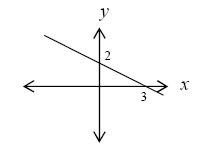
\includegraphics{TeXGraphics/ExpectationsFigurea.jpg}
	\label{Expectations}
\end{figure}

$\ldots$ or {\bf{symbolically}} like this $\ldots$
 $$2x + 3y = 6$$
 
$\ldots$ or we can find a list of points on that line {\bf{tabularly}} like this $\ldots$
 $$\begin{array}{|c|c|}
 \hline
   x & y  \\ \hline
   0 & 2  \\ \hline
   3 & 0  \\ \hline
   1 & {{\textstyle{4 \over 3}}}  \\ \hline
   {{\textstyle{3 \over 2}}} & 1  \\ \hline
    {- 3} & 4 \\ \hline
 \end{array}$$

$\ldots$ or we can describe the line {\bf{verbally}} like this $\ldots$
 \begin{quote}{This line has a slope of $ - {2 \over 3},$ an $x$-intercept of $x = 3$ and a $y$-intercept of $y = 2$.}\end{quote}

{\bf{Graphical}} representations might include the usual type of graphs, diagrams, pictures, etc.  {\bf{Symbolic}} representations might include algebraic operations, equations, evaluation of formulas, etc.  {\bf{Tabular}} representations might include lists of data points, calculations, numerical investigations, etc.  {\bf{Verbal}} descriptions include sentences and paragraphs but would also include verbal annotations of graphs, symbols and tables.

 It is your responsibility to develop a satisfactory method of writing mathematics.  It may take a few assignments for everyone to understand what is expected but I will provide you with examples of good (and bad) writing during the first couple of weeks of class to help you understand.  The writing assignments that are due each week are relatively low risk, i.e., the score for each individual assignment is a small part of your grade and you have a chance to make up these assignments.  However, one purpose of the daily writing assignments is to prepare you to do well on the writing that will be on the exams where the risk is higher.  So use the daily writings to work on your style and presentation.
 
	\section{Grading Rubric}
	 
Each writing assignment is worth 4 points.
\begin{itemize}
\item {\bf{1 point}}:  The mathematics is correct with only minor arithmetic or notational errors.  The mathematical language, notation and symbols are correct and appropriate.
\item  {\bf{1 point}}:  The writing and organization is well done with only minor grammar or spelling errors.  The writing is well organized around a central theme and flows well.  
\item  {\bf{1 point}}:  The writing answered the questions asked and there is no "fluff".
\item  {\bf{1 point}}:  Sufficient evidence is given to support the answer (i.e., graphical, symbolic, tabular and verbal representations).  Examples are used to elaborate on and to clarify the concepts discussed.  
\end{itemize}
 It is possible to get a 2.5 for a grade.  This might mean the writing had problems (loss of 1 point) and you had some evidence but could have had more (loss of 0.5 of a point).  I will try to give you comments that will help you understand why you lost points.  Of course, not all writing requires examples \emph{and} algebra \emph{and}graphs \emph{and}numerical calculations, but you should try to include these whenever appropriate.  These constitute evidence that you understand the concept fully and support the claims you make in the writing.

  \section{ Expectations of specific question types}

\begin{description}
\item[Compare and contrast] You will often be asked to compare and contrast two 
concepts.  To compare and contrast you need to describe the ways in which the 
concepts are the same (compare) and the ways in which the concepts are different 
(contrast).  Sometimes making a side-by-side list of features of the 2 concepts 
will help you organize your work. You must have sentences that start with 
"These concepts are alike because..." and "These concepts are different because...".  A description of each concept without connection to the other is unnecessary and does not satisfy the requirements of this type of question.  
\item[Annotated example]  An annotated example has sentences that explain each step of the calculation.  On way to write a nice annotated example is first to do the mathematics.  Include a reference number at the end of each line, like this.
 $$\begin{array}{rclr}
  f(x)& = &\left( {x - 2} \right)^3 \left( {x + 3} \right)^2  & (1) \\ 
  f'(x)& =& 3\left( {x - 2} \right)^2 \left( {x + 3} \right)^2  + 2\left( {x - 2} \right)^3 \left( {x + 3} \right) & (2) \\ 
   &= &5\left( {x - 2} \right)^2 \left( {x + 3} \right)\left( {x + 1} \right) &  (3) 
\end{array} 
$$

Now, write a paragraph about the work you did.  You can easily refer to specific work by using the reference numbers.  "We took the function (1) and found the derivative (2) by using the product rule.  Equation (3) is a factored version of (2)."  Tell the reader what you did, what rules or theorems you used, and anything else that will help him or her understand the results.  Write actively and use first person plural.  Notice that I did not include every single excruciating detail of the calculus and algebra.  Remember that what you turn in must be a final product so you can choose the most important steps to include.
\item[Concept map]  A concept map is a diagram of your own design that shows the interrelationships of a set of concepts.  Sentences describing the relationships and other aspects of the concepts are included in the map.  You can include any helpful information such as comparisons, contrasts, extensions, generalizations, parallels, etc.  Remember that the concept maps fall under the category of writing, so there has to be a significant amount of writing in the map even if it is not in the standard paragraph form of an essay.
\item[Generalization]  When asked to generalize you need to describe what happens in the general case.  For example, we know that the solution to $x^2 - 4 = 0$ is $x = 2$ and $x = -2$.  A generalization of this is that the solution to $x^2 - k = 0$ is $$
x = \sqrt k 
$$
 and $$
x =  - \sqrt k 
.$$
  To find a generalization, I used an unknown constant in the place of a number and described the solution in that general case.  Sometimes to generalize we see what happens in the $n$th case.  We know that 
$ax + b = 0$ has at most 1 real solution and $ax^2 + bx + c = 0$ has at most 2 real solutions.  To generalize, we might try to show that a polynomial equation of degree $n$ has at most $n$ real solutions.
\item [True or false]  Some of the questions ask you to determine if a statement is always true or not always true.  If it is always true, you need to provide an argument to justify this claim.  If it is not always true, you should provide an example and a counterexample.  If the statement is never true, you need to provide an argument to justify this claim.
\end{description}

 \section{References}

These expectations was developed using the ideas in Jerry Stonewater's writing \cite{SJ}.
  


  \begin{thebibliography}{99}



\bibitem{B}       http://www.woodrow.org/teachers/mi/1993/37burc.html

\bibitem{Bi}      Bittinger, Marvin L., \emph{Calculus and Its Applications}, Addision-Wesley, 2004.

\bibitem{BW}   Barker, William H. and James E.Ward, \emph{The Calculus Companion}, 5th edition, Wiley, 1995.

\bibitem{EP}     Edwards, C. Henry and David E. Penney, \emph{Calculus Early Transcendentals Version}, 6th edition, Prentice Hall, 2003.  (Concept questions are included in every section of the text.)

\bibitem{EP2}	Edwards, C. Henry and David E. Penney, \emph{Calculus Matrix Version}, 6th edition, Prentice Hall, 2003.  (There are a large number of true/false questions on the accompanying CD.)

\bibitem{FWG} Finney, Wier, Giordano, \emph{Calculus}, 10th edition, Addison Wesley Longman, 2001.

\bibitem{MC6}	``Mathematics in College'', Instructional Resource Center and the CUNY Mathematics Discussion Group, City University of New York,  Spring-Summer, 1986.

\bibitem{MC7}	``Mathematics in College'', Instructional Resource Center and the CUNY Mathematics Discussion Group, City University of New York,  Spring-Summer, 1987.

\bibitem{MR}    Meier, John and Thomas Rishel, \emph{Writing in the Teaching and Learning of Mathematics}, Mathematical Association of America, 1998.

\bibitem{R}       Riddle, Douglas F., \emph{Calculus and Analytic Geometry}, 2nd edition, Wadsworth, 1974.

\bibitem{S}       Sterret, Andrew, editor, \emph{Using Writing to Teach Mathematics}, Mathematical Association of America, 1990.

\bibitem{SBS}   Strauss, Bradley, Smith, Calculus, 3rd edition, Prentice Hall, 2002.

\bibitem{SMo}  Smith, David A. and Lawrence C. Moore, \emph{Instructor's Guide with Test Items to accompany Calculus Modeling and Application}, D.C. Heath, 1996.

\bibitem{SM}    Smith, Robert T. and Roland B. Minton, \emph{Calculus}, premiere edition,McGraw Hill, 2000. (Writing prompts are included in every section of this text.)

\bibitem{SM1}  Smith, Robert T. and Roland B. Minton, \emph{Calculus}, McGraw Hill, 2006. (Writing prompts are included in every section of this text.)

\bibitem{SO}    Spiegel, Murray R., \emph{Schaum's Outline of Theory and Problems of Complex Variables}, McGraw-Hill, 1999.

\bibitem{SJ}   Stonewater, Jerry K., ``The Mathematics Writer's Checklist:  The Development of a Preliminary Assessment Tool for Writing in Mathematics'',\emph{ School Science and Mathematics}, Volume 102, Number 7, November 2002.



\end{thebibliography}

\end{document}


\end{document}